\documentclass[10.5pt,twoside]{report}
\usepackage{amsmath,amssymb,amsthm,amsbsy,graphicx}
\usepackage{geometry}

\geometry{paperwidth=18.91cm,paperheight=24.589cm,
vmargin=1.9cm, % top and bottom margins
inner=1.9cm, % inside margin
outer=2.29cm, % outside margin
bindingoffset=0.89cm % gutter
}
\usepackage{minitoc}
\renewcommand{\contentsname}{}
\usepackage[english]{babel}
\usepackage{fancyhdr}
\addto\captionsenglish{\renewcommand{\chaptername}{Module}}
\theoremstyle{definition}
\newtheorem{exmp}{Example}[section]
\setlength{\parindent}{0pt}
\setlength{\mtcindent}{-18pt}
\nomtcrule
\renewcommand{\mtctitle}{}
\graphicspath{{images/}}
\usepackage{hyperref}
\hypersetup{colorlinks, allcolors=blue, linktocpage}
\raggedbottom





\begin{document}


\title{wxMaxima for Calculus I}

\author{Zachary Hannan\\ Solano Community College}



\date{}

\maketitle

\pagebreak
\vspace*{\fill}
\pagenumbering{gobble}

This work is licensed under the Creative Commons Attribution-NonCommercial-ShareAlike 4.0 International License. To view a copy of this license, visit \url{http://creativecommons.org/licenses/by-nc-sa/4.0/}.
${}$\\

The CC-BY-NC-SA license allows anyone to modify and/or redistribute this material as long as the original author and all subsequent authors are attributed.  This work and its derivatives must not be used for commercial purposes except by permission of the original author (the copyright holder), and all derivative works must use the identical license. If you wish to create a derivative work, the .tex files are available here:  \url{https://wxmaximafor.wordpress.com/}.  I would appreciate  it if you contact me at zhannan@solano.edu if you decide to create a derivative work.




\vspace*{\fill}
\pagebreak
\pagenumbering{roman}
\setcounter{page}{3}

\dominitoc
\tableofcontents
\setcounter{chapter}{-1}



\pagebreak

\chapter*{Preface}
\addcontentsline{toc}{chapter}{Preface}

\section*{\large{Computer Algebra Systems:}}

A computer algebra system is a collection of software designed primarily for symbolic manipulation.  A CAS can do just about any symbolic calculation one might do ``by hand'', but the CAS is much faster, more accurate and capable of handling greater complexity.  Complex calculations can be broken into manageable pieces by using function assignments, and systems can be explored by quickly changing their parameters.  In addition to symbolic manipulation, a CAS can produce quality graphics, make numerical approximations of various types and run simple programs to solve problems that cannot be solved symbolically.


\section*{\large{wxMaxima:}}

wxMaxima is a user interface for the computer algebra system
Maxima.   The interface allows the user to build, edit and save a 
document (a .wxm file) containing many calculations and graphics, 
and \textit{most} operations can be accessed through the GUI if desired.  Maxima and wxMaxima are open-source projects, which means they will always be free and they are always improving thanks to the pro bono work of their many enthusiasts.\\

The latest version of wxMaxima for Windows and Mac machines can be 
obtained here: \url{http://andrejv.github.io/wxmaxima/}.  When you click the 
download link for your operating system, you will be taken to a 
sourceforge.net page that will automatically download Maxima, 
wxMaxima, GNUplot and any other necessary auxilliary programs required 
for wxMaxima to run on your machine.  Installation on a Windows machine
typically takes about 5 minutes.


\section*{\large{Software Versions}}

This text is written using wxMaxima version 12.04.0 and Maxima version 
5.27.0.  If you run newer versions of the software it is 
unlikely to cause any problems.  Bugs do occur rarely, however, so I 
recommend that the instructor and students all use the same version 
in case troubleshooting becomes necessary.

\pagebreak
\section*{\large{``wxMaxima for'' Series}}

I have released two books in the ``wxMaxima for'' series:\\

\begin{tabular}{l c}
 ``wxMaxima for Calculus I''	&June 2015\\
 ``wxMaxima for Calculus II'' &June 2015\\

\end{tabular}

${}$\\
with plans to publish similar texts for Linear Algebra, Differential Equations and Multivariable Calculus over the next several years.\\

Texts can be obtained at
\url{https://wxmaximafor.wordpress.com/}. The texts are available as free .pdf downloads or an affordable ``print-on-demand'' option. \\

The texts primarily target lower division students who are concurrently taking the standard sequence of mathematics courses for engineering, physical science and applied mathematics majors.  Universities increasingly expect such students to be competent with mathematical software when they begin their upper division courses, and many institutions currently run math labs to address this need.  Each text in the ``wxMaxima for'' sequence can serve as a lab manual for a one semester, 1-unit lab course, or a valuable ``by example'' resource for students learning computer algebra independently.\\

Assuming only basic experience with computers (comfort with an operating system such as Windows or Mac OS), each text gradually introduces computer algebra by using examples relevant to the concurrent math course.  The main theoretical points of each course are reviewed concisely, and commands are introduced as they are needed.  Examples motivate and reinforce the important mathematical concepts and illustrate their applications in the context of computer algebra.  Written commands are used exclusively for two reasons:  first, they are more powerful and flexible, and secondly,  getting comfortable with written commands ensures that the computing learned here will translate easily to other software packages.  



\section*{\large{Text Layout}}

Each text is divided into 7 modules, each consisting of several sections and subsections.  Each subsection typically starts with a short theoretical discussion followed by several Examples worked in wxMaxima.  Each module ends with a short set of Exercises progressing from routine to advanced.  Exceptionally challenging sections and Exercises are marked with an asterisk.\\

This text is not intended to be an encyclopedic reference manual, but each module contains a list of ``Key Commands'' on the title page to make it easier to search for an example that uses a particular command.\\

\pagebreak

\section*{\large{To the student}}

For students with very little computer experience, the first couple modules will move very slowly.  Making mistakes and debugging your commands is a natural part of learning the syntax of a new program.  Although wxMaxima will attempt to help you with errors, the most valuable resource you have is internet research.  If you Google a particular problem, you will find a variety of forums on the web where you will likely find a similar problem addressed.  With time, your wxMaxima vocabulary and your ability to search efficiently will grow.  Note that it is wise to include ``wxMaxima'' in your queries rather than ``Maxima'', as the latter term has many meanings other than the computer algebra system! \\

The official Maxima manual can be found at \url{http://maxima.sourceforge.net/docs/manual/maxima.html}, though you 
should be warned that it is written for an audience with a high degree
of computing knowledge.  I occasionally use the official manual, but I have found that searching for relevant examples is the fastest way to learn.\\

It is important to work through the Examples yourself, whether or not they are assigned by your instructor.  When you type out the commands for yourself, you will undoubtedly make syntax errors that have to be debugged.  Fixing your syntax in a worked example is excellent preparation for doing the Exercises on your own.\\


\section*{\large{To the Instructor}}

There are varying levels at which this material can be incorporated in your course.  You may decide to have the students simply reproduce and submit all Examples from the text, or you may decide to only assign selected Exercises and let the students use the text for reference on their own.  The material can be casual or very demanding depending on how much you include in your course. \\

I recommend that students submit their work by e-mail in a well-formatted wxMaxima worksheet (.wxm) file with a clear header and Examples and/or Exercises clearly labeled.  Students can insert text lines in their worksheet by selecting \verb|Cell > Insert Text Cell| or hitting \verb|Ctrl+1|.  When you open the worksheet, the commands will have to be re-executed, and this is a quick way to verify that all the code works and the desired solutions are obtained.  Students have the responsibility to debug their work until it runs without error.\\

\line(1,0){60}
\linethickness{0.5mm}
${}$\\

Any feedback on this text is greatly appreciated and will be
taken into consideration for future editions.  \\

Thank you,\\

Zak Hannan\\
Instructor of Mathematics and Physics\\
Solano Community College, Fairfield, CA\\
zhannan@solano.edu








\pagebreak

\pagenumbering{arabic}

\setcounter{mtc}{1}

\chapter{Introduction to wxMaxima}


\vspace*{\fill}

\minitoc

\vspace*{\fill}


\flushleft{\textbf{\Large Key Commands Included in This Module}}
\newline
\newline

\begin{tabular}{l l l l l}
 \verb|float   |   &\verb|trigsimp   |   &\verb|kill(all)   |  &\verb|parametric   |  &\verb|rhs   |  \\
 \verb|ratsimp   |   &\verb|trigreduce   |   &\verb|wxdraw2d   |  &\verb|dimensions   |  &\verb|makelist   |  \\
 \verb|fullratsimp   |   &\verb|trigexpand   |   &\verb|wxdraw3d   |  &\verb|solve   |  &\verb|for-do   |  \\
 \verb|expand   |   &\verb|subst   |   &\verb|explicit   |  &\verb|find_root   | &\verb|sum   |   \\
 \verb|factor   |   &\verb|sublis   |   &\verb|implicit   | &\verb|lhs   |  &\verb|simpsum   |   \\
\end{tabular}



\pagebreak


\section{Basic Operations}\label{Basic Operations}

\subsection{Arithmetic}

wxMaxima uses \verb|+,-,*,/,^,sqrt,log| for add, subtract, multiply, divide, exponentiate, square root and natural log.  We use \verb|%| to call a prior result and \verb|float| to find a decimal approximation.  To show the results of each calculation, we end the input line with \verb|;| and hit \verb|shift+enter|.  If we wish to hide the output of a calculation, we end the line with \verb|$| instead of \verb|;|.

\begin{exmp}  Perform the following arithmetic operations:\\
${}$\\



1.  Compute $3 \cdot 2 + 5$.\\
2.  Add $\sqrt{2}$ to the previous output.\\
3.  Find a decimal approximation for the previous output.\\
4.  Square the previous output.

\begin{verbatim}
  (%i1) 3*2+5;
  (%o1) 11
  (%i2) %+sqrt(2);
  (%o2) sqrt(2)+11
  (%i3) float(%);
  (%o3) 12.4142135623731
  (%i4) %^2;
  (%o4) 154.1126983722081
\end{verbatim}

You will find that your output is occasionally ``prettier'' than the output shown in this text; for example, \verb|sqrt(2)+11| should display as $\sqrt{2}+11$.  We use the ``pretty'' format only when necessary for clarity.

\end{exmp}

\line(1,0){60}
\linethickness{0.5mm}

\begin{exmp} Add $\frac{5}{6}$ and $\frac{7}{15}$ and find the reduced form of the result, then express your answer as a decimal approximation.\\


\begin{verbatim}
(%i5) (5/6)+(7/15);
(%o5) 13/10
(%i6) float(%);
(%o6) 1.3
\end{verbatim}

Note that wxMaxima automatically puts the exact fraction form in lowest terms for us.

\end{exmp}

\line(1,0){60}
\linethickness{0.5mm}


\begin{exmp}   wxMaxima uses the symbol \verb|%e| for the ubiquitous constant $e$.  Find a decimal approximation for $e$ and verify that $\ln{e}=1$.\\


\begin{verbatim}
(%i7) float(%e);
(%o7) 2.718281828459045
(%i8) log(%e);
(%o8) 1
\end{verbatim}

\end{exmp}

\line(1,0){60}
\linethickness{0.5mm}
${}$\\



\subsection{Algebra}

wxMaxima can handle basic algebraic operations on variable expressions as well as numbers:  combining like terms, expanding and factoring, adding/substracting/reducing rational expressions, etc.  In some cases a complete simplification is automatic, and in other cases we have to coax a simplification using \verb|ratsimp| or \verb|fullratsimp| (the latter command simply applies \verb|ratsimp| repeatedly).  Note that an input like \verb|5x| results in an error -- we have to explicitly note the multiplication by writing \verb|5*x|.

\begin{exmp} Perform the following operations:\\
${}$\\
 

1. Simplify:  $(3a+b)+2(2a-b)$\\
${}$\\
\verb|  | We enter the expression and apply \verb|ratsimp| to combine like terms:

\begin{verbatim}
  (%i9) (3*a+b)+2*(2*a-b);
  (%o9) b+2*(2*a-b)+3*a
  (%i10) ratsimp(%);
  (%o10) 7*a-b
\end{verbatim}


2. Expand:  $(a+b)^3$\\
${}$\\
\verb|  | \verb|expand| cubes the binomial:

\begin{verbatim}
  (%i11) (a+b)^3;
  (%o11) (b+a)^3
  (%i12) expand(%);
  (%o12) b^3+3*a*b^2+3*a^2*b+a^3
\end{verbatim}

3.  Factor:  $x^2-8x+12$\\
${}$\\
\verb|  | We simply apply \verb|factor|:

\begin{verbatim}
  (%i13) factor(x^2-8*x+12);
  (%o13) (x-6)*(x-2)
\end{verbatim}


4.  Add and express in factored form:  $\frac{5}{x^2-1}+ \frac{x-2}{x^2+2x-3}$\\
${}$\\
\verb|  | We add using \verb|ratsimp|, then put the answer in factored form using \verb|factor|:

\begin{verbatim}
  (%i14) 5/(x^2-1)+(x-2)/(x^2+2*x-3);
  (%o14) (x-2)/(x^2+2*x-3)+5/(x^2-1)
  (%i15) ratsimp(%);
  (%o15) (x^2+4*x+13)/(x^3+3*x^2-x-3)
  (%i16) factor(%);
  (%o16) (x^2+4*x+13)/((x-1)*(x+1)*(x+3))
\end{verbatim}


5.  Reduce:  $\frac{\frac{2x^2+xy}{y}}{\frac{xy+x}{y^2}}$\\
${}$\\
\verb|  | We enter the complex fraction, reduce using \verb|ratsimp| and factor using \verb|factor|:

\begin{verbatim}
  (%i17) ((2*x^2+x*y)/y)/((x*y+x)/y^2);
  (%o17) (y*(x*y+2*x^2))/(x*y+x)
  (%i18) ratsimp(%);
  (%o18) (y^2+2*x*y)/(y+1)
  (%i19) factor(%);
  (%o19) (y*(y+2*x))/(y+1)
\end{verbatim}


\end{exmp}

\line(1,0){60}
\linethickness{0.5mm}
${}$\\

\subsection{Trigonometry}

wxMaxima knows about all the trigonometric functions.  We input angles in radians, so any angle measured in degrees must be converted to radians using a factor of $\frac{2\pi}{360}$.  \verb|%pi| is the special symbol for $\pi$.

\begin{exmp} Compute $\sin{85^\circ}$ and $\tan{\frac{11\pi}{12}}$.\\


\begin{verbatim}
(%i20) 85*2*%pi/360;
(%o20) (17*%pi)/36
(%i21) sin(%);
(%o21) sin((17*%pi)/36)
(%i22) float(%);
(%o22) 0.99619469809175

(%i23) float(tan(11*%pi/12));
(%o23) -0.26794919243112
\end{verbatim}

\end{exmp}

\line(1,0){60}
\linethickness{0.5mm}
${}$\\
${}$\\

We use \verb|trigsimp| to apply pythagorean identities, \verb|trigreduce| to reduce powers of trig functions and \verb|trigexpand| to expand functions of ``multiple angles''.\\

\begin{exmp}  A survey of trigonometric manipulations.\\
${}$\\

1.  Apply \verb|trigreduce| to $\sin^2{x}+\cos^2{x}$.  What happens?  Try using \verb|trigsimp| instead.\\  

\begin{verbatim}
  (%i24) trigreduce((sin(x))^2+(cos(x))^2);
  (%o24) (cos(2*x)+1)/2+(1-cos(2*x))/2
\end{verbatim}

\verb|  | \verb|trigreduce| resulted in a more complicated expression -- we apply \verb|trigsimp| instead:

\begin{verbatim}
  (%i25) trigsimp((cos(x))^2+(sin(x))^2);
  (%o25) 1
\end{verbatim}

2.  Express $\sin^2{x}$ in terms of a ``double angle''.\\

\verb|  | This time \verb|trigreduce| is the desired command:

\begin{verbatim}
  (%i26) trigreduce((sin(x))^2);
  (%o26) (1-cos(2*x))/2
\end{verbatim}

3.  Obtain a formula for $\cos{(x+y)}$ in terms of $\sin{x}$ and $\cos{x}$.\\

\verb|  | \verb|trigexpand| will simplify the argument of the cosine:

\begin{verbatim}
  (%i27) trigexpand(cos(x+y));
  (%o27) cos(x)*cos(y)-sin(x)*sin(y)
\end{verbatim}


\end{exmp}
\line(1,0){60}
\linethickness{0.5mm}

\pagebreak

\section{Expressions and Functions}\label{Expressions and Functions}

One of the powerful features of a computer algebra system is that we can label a variety of objects then ``call'' them later using that label.  We can assign a label to an expression using ``\verb|:|'' and we can assign a label to a function using ``\verb|:=|''.  Expressions can be evaluated for specific values of the variable(s) using \verb|subst| or \verb|sublis|, while functions are evaluated using ordinary function notation.  Expressions and functions have a variety of pros and cons that will emerge as we proceed -- often we can choose either one to solve a problem.

\begin{exmp}  Assign $A$ to the expression $2x+5$ and $B$ to the expression $6-x^4$, then compute $A+B$, $A-B$ and $AB$ in expanded form.\\
${}$\\

We assign $A$ and $B$ on two consecutive lines before executing with \verb|shift+enter|.

\begin{verbatim}
(%i1) A:2*x+5$
      B:6-x^4$

(%i3) A+B;
(%o3) -x^4+2*x+11

(%i4) A-B;
(%o4) x^4+2*x-1

(%i5) A*B;
(%o5) (2*x+5)*(6-x^4)
(%i6) expand(%);
(%o6) -2*x^5-5*x^4+12*x+30
\end{verbatim}

\end{exmp}

\line(1,0){60}
\linethickness{0.5mm}

\begin{exmp}  Use \verb|subst| to evaluate $A$ when $x=-3$ and when $x=B$.\\


\begin{verbatim}
(%i7) subst(-3,x,A);
(%o7) -1

(%i8) subst(B,x,A);
(%o8) 2*(6-x^4)+5
\end{verbatim}

\end{exmp}

\line(1,0){60}
\linethickness{0.5mm}
${}$\\

\begin{exmp}  Assign $f(x)$ to the square root function.  Evaluate $f(4)$, $f(-4)$ and $f(A)$.\\


\begin{verbatim}
(%i9) f(x):=sqrt(x);
(%o9) f(x):=sqrt(x)

(%i10) f(4);
(%o10) 2

(%i11) f(-4);
(%o11) 2*%i

(%i12) f(A);
(%o12) sqrt(2*x+5)
\end{verbatim}

We see that $\sqrt{-4}$ evaluates to $2i$.  Note that the special symbol for the imaginary unit $i$ is \verb|%i|.  wxMaxima is not restricted to only real solutions!

\end{exmp}

\line(1,0){60}
\linethickness{0.5mm}

\begin{exmp} Use \verb|sublis| to evaluate $\frac{-b+\sqrt{b^2-4ac}}{2a}$ when $a=1$, $b=-3$ and $c=5$.\\
${}$\\
\begin{verbatim}
(%i9) EXPN:(-b+sqrt(b^2-4*a*c))/(2*a)$

(%i10) sublis([a=1,b=-3,c=5],EXPN);
(%o10) (sqrt(11)*%i+3)/2
\end{verbatim}

\end{exmp}

\line(1,0){60}
\linethickness{0.5mm}

${}$\\

Functions can have an arbitrary number of variables.  Sometimes we use a variable as a \textit{parameter} to create a family of related functions:

\begin{exmp} Define $f_n(x)=\cos{(n\pi x)}$, then list $f_n(x)$ for several values of $n$.\\


\begin{verbatim}
(%i13) f(n,x):=cos(n*%pi*x)$
       f(1,x);
       f(2,x);
       f(3,x);
(%o14) cos(%pi*x)
(%o15) cos(2*%pi*x)
(%o16) cos(3*%pi*x)
\end{verbatim}

\end{exmp}


\line(1,0){60}
\linethickness{0.5mm}



\pagebreak


\section{2D and 3D Plots}\label{2D and 3D Plots}

wxMaxima creates plots by calling another program called GNUplot.  In this text, we exclusively use the commands \verb|wxdraw2d| and \verb|wxdraw3d| to create embedded 2D and 3D plots.  The related commands \verb|draw2d| and \verb|draw3d| will create the same plot in a GNUplot pop-up window.  The pop-up window is useful for manipulating 3D plots (we can move the picture around with a mouse), but the embedded plots are more useful for printing our work.  In older versions of wxMaxima, it may be necessary to enter \verb|load(draw)$| before using the \verb|wxdraw2d| and \verb|wxdraw3d| commands.\\
${}$\\
Plots can be ammended with a host of attributes introduced gradually throughout the text.  We include a small sample of graphic objects and plot features below.

\begin{exmp} Define $f(x)=x^2$, then make a simple plot of $f(x)$ on $[-3,3]$.\\
${}$\\

We begin this section by applying \verb|kill(all)| to delete all the assignments wxMaxima is currently remembering.  In practice, we only need to use \verb|kill(all)| if our previous assignments are causing some kind of interference with a calculation.  We use \verb|explicit| to plot the function because $f(x)$ is stated \textit{explicitly} as a function of $x$, then the domain is listed alongside the function.  We place several line breaks inside \verb|wxdraw2d| to aid our organization:

\begin{verbatim}
(%i1) kill(all)$
(%i1) f(x):=x^2$
(%i2) wxdraw2d(
      explicit(f(x),x,-3,3)
      );
\end{verbatim}

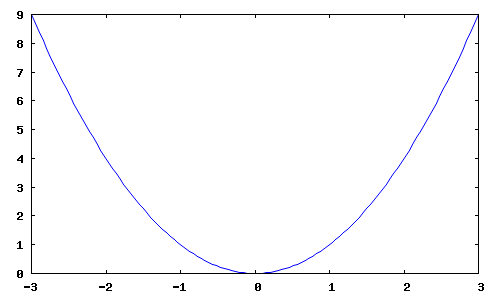
\includegraphics[width=3in]{example_0_3_1_1}

\end{exmp}

\line(1,0){60}
\linethickness{0.5mm}
${}$\\

\begin{exmp} Plot the points $[-3,1]$ and $[2,5]$ on a grid for $x$-range $[-10,10]$ and $y$-range $[-10,10]$. Include a label above each point.\\
${}$\\

We use \verb|point_type=7| to make closed circles and \verb|points| to list the desired points.  \verb|label| is used to create the text of each label and attach it to the desired coordinates (in this case, 1 unit above the actual points):

\begin{verbatim}
(%i3) wxdraw2d(
      grid=true,
      xrange=[-10,10],
      yrange=[-10,10],
      point_type=7,
       points([[-3,1],[2,5]]),
      label(["[-3,1]",-3,2],["[2,5]",2,6])
      );
\end{verbatim}

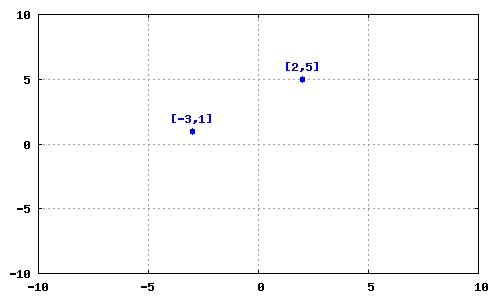
\includegraphics[width=3in]{example_0_3_2_1}

\end{exmp}

\line(1,0){60}
\linethickness{0.5mm}



\begin{exmp}  Plot a black vertical line $x=3$, and plot the unit circle in red with $x$-range $[-4,4]$ and $y$-range $[-4,4]$.  Include the $x$ and $y$ axes, a grid and a title.  \\
${}$\\

This example is a good illustration of how easily a plot can grow in complexity.  A vertical line is not a function, so it must be defined \textit{parametrically}.  We tell wxMaxima to plot many points $(3,t)$ as $t$ runs from $-4$ to $4$.  In addition, the equation of the unit circle defines a curve \textit{implicitly}:  we can't solve for $y$ in terms of $x$.  Finally, the unit circle will be distorted if we don't force the aspect ratio to be square using \verb|dimensions|:

\begin{verbatim}
(%i4) wxdraw2d(
      grid=true,
      xaxis=true,
      yaxis=true,
      dimensions=[600,600],
      xrange=[-4,4],
      yrange=[-4,4],
      title="The unit circle and the line x=3.",
      color=black,
       parametric(3,t,t,-4,4),
      color=red,
       implicit(x^2+y^2=1,x,-1,1,y,-1,1)
      ); 
\end{verbatim}

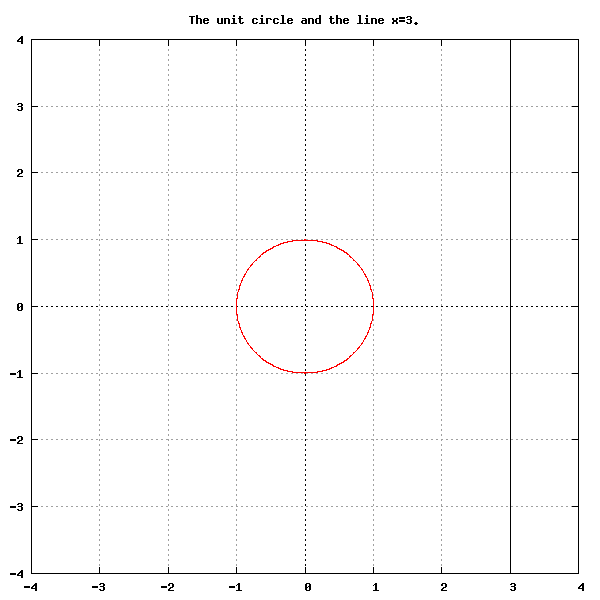
\includegraphics[width=3in]{example_0_3_3_1}

\end{exmp}

\line(1,0){60}
\linethickness{0.5mm}




\begin{exmp}  Make a quick plot of the paraboloid $z=x^2+y^2$ using \verb|wxdraw3d|.  In addition, use \verb|draw3d| to draw the paraboloid in a GNUplot window, then manipulate the plot with a mouse.\\



\begin{verbatim}
(%i5) wxdraw3d(
      explicit(x^2+y^2,x,-5,5,y,-5,5)
      );
\end{verbatim}

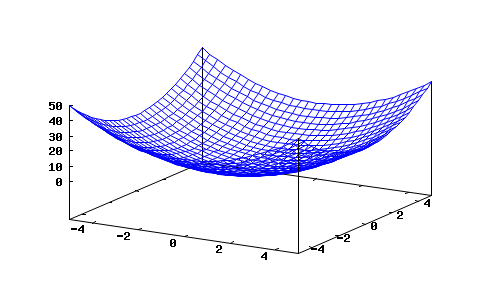
\includegraphics[width=3in]{example_0_3_4_1}

\end{exmp}

\line(1,0){60}
\linethickness{0.5mm}

\pagebreak


\section{Defining and Solving Equations}\label{Defining and Solving Equations}

In wxMaxima, the symbol ``\verb|=|'' is reserved for defining equations.  Once an equation is defined, we can use \verb|rhs| and \verb|lhs| to isolate the right and left sides.  Many equations and systems of equations can be solved using \verb|solve|, but some equations can only be solved with numerical approximations using \verb|find_root| or another approximation.

\begin{exmp} Assign the symbol \verb|EQN| to the equation $3x-6=6x+5$, then solve the equation ``manually'' by performing the usual algebraic operations to isolate $x$.  Check your answer by substituting this value of $x$ into the left and right sides of the original equation.  Finally, check your answer again by using \verb|solve|.\\
${}$\\

We run through the standard process for linear equations:

\begin{verbatim}
(%i1) EQN:3*x-6=6*x+5;
(%o1) 3*x-6=6*x+5
(%i2) %+6;
(%o2) 3*x=6*x+11
(%i3) %-6*x;
(%o3) -3*x=11
(%i4) %/-3;
(%o4) x=-11/3
\end{verbatim}

We check our answer using \verb|subst|:

\begin{verbatim}
(%i5) subst(-11/3,x,rhs(EQN));
(%o5) -17
(%i6) subst(-11/3,x,lhs(EQN));
(%o6) -17
\end{verbatim}

Finally, we repeat the solution using \verb|solve|:

\begin{verbatim}
(%i7) solve(EQN,x);
(%o7) [x=-11/3]
\end{verbatim}


\end{exmp}


\line(1,0){60}
\linethickness{0.5mm}

\begin{exmp} Attempt to solve $\ln{x}=\sin{x}$ using \verb|solve|.  What happens?  Now rephrase the problem in terms of finding a \textit{root} of another function.  Approximate the solution using \verb|find_root|.\\
${}$\\

First we attempt the naive solution, calling the equation \verb|EQN2|:

\begin{verbatim}
(%i8) EQN2:log(x)=sin(x)$
      solve(EQN2,x);
(%o9) [sin(x)=log(x)]
\end{verbatim}

wxMaxima simply repeats the question, indicating a failure to find the solution (in fact, \verb|solve| can only solve \textit{some} polynomial equations!).  However, we realize that any solution to $\ln{x}=\sin{x}$ is also a solution of $\ln{x}-\sin{x}=0$, so we can examine the function $f(x)=\ln{x}-\sin{x}$ and numerically approximate its roots.\\
${}$\\
One complication of \verb|find_root| is that we have to specify the interval on which the root occurs, and the function must be defined on the interval we choose.  We can choose an interval by quickly sketching the function:


\begin{verbatim}
(%i10) wxdraw2d(
      grid=true,
      explicit(log(x)-sin(x),x,0,10)
      );
\end{verbatim}

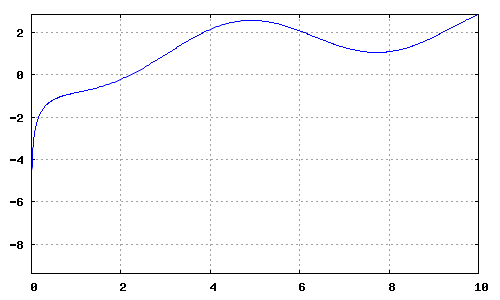
\includegraphics[width=3in]{example_0_4_2_1}

We see a root somewhere on $[2,4]$.  Note:  if we choose the interval $[0,4]$, \verb|find_root| fails because $\ln{x}$ is not defined at $x=0$!

\begin{verbatim}
(%i11) find_root(log(x)-sin(x),2,4);
(%o11) 2.219107148913746
\end{verbatim}

We obtain $x \approx 2.219$ as the numerical solution to the equation.

\end{exmp}

\line(1,0){60}
\linethickness{0.5mm}

\begin{exmp} Solve the system of equations
$\begin{cases} 2x-3y&=5 \\ 3x+y&=2 \end{cases}$ using \verb|solve|.  Plot both equations implicitly and mark the intersection point in the plot.\\

\begin{verbatim}
(%i12) L1:2*x-3*y=5$
       L2:3*x+y=2$
       solve([L1,L2],[x,y]);
(%o14) [[x=1,y=-1]]

(%i15) wxdraw2d(
       grid=true,
       color=black,
        implicit(L1,x,-2,2,y,-2,2),
        implicit(L2,x,-2,2,y,-2,2),
       color=red,
       point_type=7,
        points([[1,-1]])
       );
\end{verbatim}

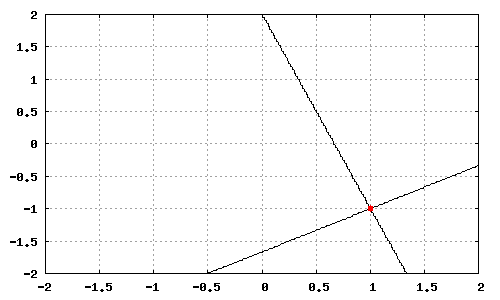
\includegraphics[width=3in]{example_0_4_3_1}

\end{exmp}


\line(1,0){60}
\linethickness{0.5mm}

\pagebreak

\section{Sequences and Sums}\label{Sequences and Sums}

\subsection{Sequences}

Sequences find a wide variety of applications, and we use them frequently in this text.  wxMaxima generates sequences using \verb|makelist| or \verb|for-do|.  \verb|makelist| offers the advantage that we can call list elements later in the calculation, while \verb|for-do| is much more flexible and powerful.

\begin{exmp} Use \verb|makelist| to generate the sequence $L=1,3,5,\dots 51$. Use wxMaxima to isolate the tenth element of the sequence. \\
${}$\\

We use the formula $2n-1$ with $n=1\dots 26$ to generate the sequence:

\begin{verbatim}
(%i1) L:makelist(2*n-1,n,1,26);
(%o1) [1,3,5,7,9,11,13,15,17,19,21,23,25,27,29,31,33,35,
        37,39,41,43,45,47,49,51]
\end{verbatim}

Now we call the tenth element of \verb|L|:

\begin{verbatim}
(%i2) L[10];
(%o2) 19
\end{verbatim}

\end{exmp}

\line(1,0){60}
\linethickness{0.5mm}


\begin{exmp} Use \verb|makelist| to generate a sequence of 20 ordered pairs on the line $y=2x$ for $x=0.0,0.1,\dots ,2$.  Feed your list of ordered pairs into \verb|wxdraw2d|. \\
${}$\\

We can generate the $x$ values using the sequence $0.1k$ for $k=0,1,\dots ,20$.  The output of \verb|makelist| is already in ``list'' form, so it is ready to feed into \verb|wxdraw2d|:

\begin{verbatim}
(%i3) POINTS:makelist([0.1*k,2*(0.1*k)],k,0,20);
(%o3) [[0,0],[0.1,0.2],[0.2,0.4],[0.3,0.6],[0.4,0.8],[0.5,1.0],
      [0.6,1.2],[0.7,1.4],[0.8,1.6],[0.9,1.8],[1.0,2.0],[1.1,2.2],
      [1.2,2.4],[1.3,2.6],[1.4,2.8],[1.5,3.0],[1.6,3.2],[1.7,3.4],
      [1.8,3.6],[1.9,3.8],[2.0,4.0]]

(%i4) wxdraw2d(
      grid=true,
      xaxis=true,
      yaxis=true,
      xrange=[-1,3],
      yrange=[-1,5],
      point_type=7,
      color=red,
      points(POINTS)
      );
\end{verbatim}

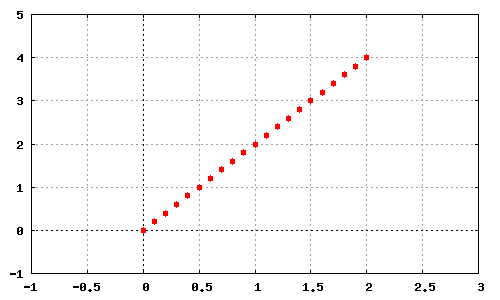
\includegraphics[width=3in]{example_0_5_2_1}

\end{exmp}

\line(1,0){60}
\linethickness{0.5mm}


\begin{exmp} Use a \verb|for-do| loop to generate the same sequence as Example 0.5.1.\\
${}$\\

When we program a \verb|for-do| loop (also called simply a ``do-loop''), we ask wxMaxima to repeat a process until some ending point is reached.  In this case, we ask wxMaxima to assign $x$ to $2n-1$ and print $x$, repeating the calculation for $n=1\dots 26$:

\begin{verbatim}
(%i5) (for n:1 thru 26 do
       (x: 2*n-1,
        print(x))
       );
       1
       3
       5
       7
       9
       11
       13
       15
       17
       19
       21
       23
       25
       27
       29
       31
       33
       35
       37
       39
       41
       43
       45
       47
       49
       51
       
(%o5)  done
\end{verbatim}

\end{exmp}

\line(1,0){60}
\linethickness{0.5mm}

\begin{exmp} The Fibonacci sequence is defined by a recursive formula $f_n=f_{n-1}+f_{n-2}$; that is, the next number is obtained by adding the previous two numbers.  If we start the sequence with $0,1,\dots$, the entire sequence is given by $0,1,1,2,3,5,8,\dots$.  Use a do-loop to generate the first twenty terms of the Fibonacci sequence.\\
${}$\\

Our use of \verb|for-do| is more substantial in this example:  we have to repeat a calculation several times and use the output of each step to compute the next step.  We define the two starting numbers $f_{n-1}$ and $f_{n-2}$ first, then the loop prints the next Fibonacci number $X$, changes the ${(n-1)}^{\mathrm{th}}$ term to the ${(n-2)}^{\mathrm{th}}$ term and assigns the ${(n-1)}^{\mathrm{th}}$ term to $X$.  Then the process is repeated 18 times for a total of 20 Fibonacci numbers.

\begin{verbatim}
(%i6) N_1:1$
      N_2:0$
(%i8) 
      (for i:1 thru 18 do
       (X:N_2+N_1,
        print(X),
        N_2:N_1,
        N_1:X)
       );
       1
       2
       3
       5
       8
       13
       21
       34
       55
       89
       144
       233
       377
       610
       987
       1597
       2584
       4181
       
(%o8)  done
\end{verbatim}


\end{exmp}

\line(1,0){60}
\linethickness{0.5mm}
${}$\\

\subsection{Sums}

wxMaxima computes sums using \verb|sum|.  The notation is very close to sigma notation:

\begin{exmp} Use \verb|sum| to compute the sum $2+4+6+\dots +50$.\\
${}$\\

In sigma notation, the sum is written $\sum_{n=1}^{25} 2n$, and the arguments of \verb|sum| simply refer to all the parts of this notation:

\begin{verbatim}
(%i9) sum(2*n,n,1,25);
(%o9) 650
\end{verbatim}

\end{exmp}

\line(1,0){60}
\linethickness{0.5mm}

\begin{exmp}  Find an algebraic formula for the sum $1+2+\dots +n$, then use a substitution to obtain the sum of the first 100 natural numbers.\\
${}$\\

In sigma notation, we wish to compute $\sum_{k=1}^n k$.  The classic formula is obtained using \verb|sum| followed by \verb|simpsum|, then we substitute $n=100$:

\begin{verbatim}
(%i10) sum(k,k,1,n),simpsum;
(%o10) (n^2+n)/2
(%i11) subst(100,n,%);
(%o11) 5050
\end{verbatim}

\end{exmp}

\line(1,0){60}
\linethickness{0.5mm}
\pagebreak

\section{Application: Line Passing Through Two Given Points}\label{Application:  Line Passing Through Two Given Points}

As a demonstration of the utility of symbolic calculation, we design a function to quickly plot the line connecting two points.\\
${}$\\
\begin{exmp}  Create a function \verb|LINE(a,b,c,d,x)| that computes the equation of a line passing through the points $(a,b)$ and $(c,d)$.  Set up your code so the simple assignment of $a,b,c,d$ will immediately produce a nice plot of the line and the two given points.  Apply your code to the points $(-0.51,-3.47)$ and $(7.12,3.94)$.\\
${}$\\


First, we define each point as a function of two variables.  The output of each function is in the correct form to use as a point within \verb|wxdraw2d|.  Then we compute the slope between the points as a function of all four variables:\\

\begin{verbatim}
(%i1) POINT1(a,b):=[a,b]$
      POINT2(c,d):=[c,d]$
      SLOPE(a,b,c,d):=(d-b)/(c-a)$  
\end{verbatim}

The next step is to plug into the point-slope formula $y-y_0=m(x-x_0)$ and solve for $y$ as a function of $x$.  We use \verb|POINT1| as $(x_0,y_0)$.
           
\begin{verbatim}           
(%i4) LINE(a,b,c,d,x):=SLOPE(a,b,c,d)*(x-a)+b$
\end{verbatim}

Finally, we make the assignments for $a,b,c,d$ and set up \verb|wxdraw2d|.  Note that everything remains general within \verb|wxdraw2d|, so we can plot the line between any two points immediately by making new assignments for $a,b,c,d$:

\begin{verbatim}
(%i5) a:-.51$
      b:-3.47$
      c:7.12$
      d:3.94$

      wxdraw2d(
      grid=true,
      xaxis=true,
      yaxis=true,
      color=black,
       explicit(LINE(a,b,c,d,x),x,a-1,c+1),
      color=red,
      point_type=7,
      points([[a,b],[c,d]])
      );
\end{verbatim}

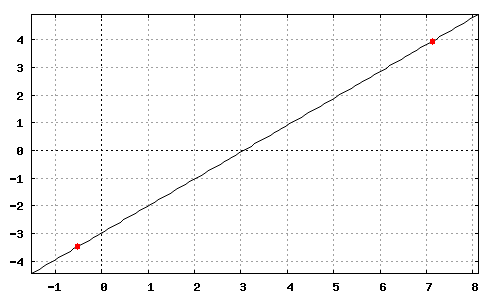
\includegraphics[width=3in]{example_0_6_1_1}
${}$\\


\end{exmp}

\line(1,0){60}
\linethickness{0.5mm}

\pagebreak






\section{Module 0 Exercises}\label{Module 0 Exercises}

\begin{enumerate}

\item  Define the expressions $A=\sqrt{3}$ and $B=5$, then find decimal approximations for $A+B$ and $A/B$.

\item  Define expressions $A=x^2$ and $B=e^x$.  Substitute $B$ for $x$ in the formula for $A$, then evaluate the resulting expression at $x=0.1$ and obtain a decimal approximation.

\item  Use \verb|trigexpand| to find a formula for $\sin{(x+y)}$ in terms of $\sin{x}$, $\sin{y}$, $\cos{x}$ and $\cos{y}$.  Use your result to compute $\sin{\frac{5\pi}{12}}$ by using the fact that $\frac{5\pi}{12}=\frac{\pi}{6}+\frac{\pi}{4}$.  Re-calculate $\sin{\frac{5\pi}{12}}$ directly and use \verb|float| to verify your answer.


\item  Add and simplify:  $\frac{2x^2-x-6}{x^2-9}+\frac{x^3-x^2-4x+4}{x^2+5x+6}$.  Express your answer in factored form.

\item Solve the equation $ax^2+bx+c=0$ for $x$.  


\item Make a plot of $f(x)=\sin{(\ln{x})}-0.2$ on $[10,30]$ including the x-axis.  Use \verb|find_root| to approximate the solution of $\sin{(\ln{x})}=0.2$ on this interval.  Verify your answer by evaluating $\sin{(\ln{x})}$ at the value of $x$ you found.

\item  Define $f(x)=x+2$ and $g(x)=x^2$.  Find the intersections of these two curves, then make a plot of both functions including the intersection points as closed circles.  Label each intersection point using decimal coordinates rounded to the second decimal place.

\item  Use \verb|makelist| and \verb|for-do| to generate the first thirty terms of the sequence $1,\frac{1}{2},\frac{1}{4},\dots$.

\item  The recursive formula for a sequence is given by $f_n=2f_{n-1}$ with a starting point of $f_0=3$.  Use a do-loop to generate the first 10 terms of this sequence recursively (as in Example 0.5.4).  Once the sequence is written down, you can guess an explicit formula for $f_n$.  Once you find this formula, use \verb|makelist| to generate the same sequence.

\item Use \verb|makelist| to plot 40 circles centered at the origin with radii $0.1,0.2,0.3,\dots$ in a single plot.  This problem is tricky because your list must produce elements that \verb|wxdraw2d| understands:  \verb|implicit| and its proper arguments must be included with each list element!

\item Any parabola can be written $f(x)=ax^2+bx+c$.  The parameters $a,b,c$ completely define the parabola.  If you are given three points lying on an unknown parabola, they generate a system of three equations in $a,b,c$.  \verb|solve| can quickly produce the solution of this system.  Write a solution similar to Example 0.6.1 to take any three points and produce a plot of the points together with the parabola passing through them.  The proper syntax for solving a system of equations is \verb|solve([eqn1,eqn2,eqn3],[var1,var2,var3])|.  Apply your code to the points $(-6.8,-5.5)$, $(0.1,6.7)$ and $(3.2,-0.9)$.



\end{enumerate}


\pagebreak



\chapter{Function Review}

\vspace*{\fill}

\minitoc

\vspace*{\fill}



\flushleft{\textbf{\large Key Commands Included in This Module}}
\newline
\newline

\begin{tabular}{l l l l}
 \verb|wxdraw2d   | &\verb|factor   |   &\verb|solve   | &\verb|dimensions   | \\
 \verb|num   |&\verb|denom   |   &\verb|ratsimp   |  &\verb|float   |\\
 \verb|limit   |&\verb|find_root   |   & \\
\end{tabular}

\pagebreak



\section{Polynomial and Rational Functions}\label{Polynomial and Rational Functions}

\subsection{Polynomial Functions}

A \textbf{polynomial function} is a function of the form:

$$P(x)=a_{n}x^{n}+a_{n-1}x^{n-1}+\dots+a_{1}x+a_{0}$$

Plotting a polynomial function in wxMaxima is straightforward, but it is notable that the factored form of the function can be useful for locating its zeros.

\begin{exmp}
Plot the function $P(x)=x^{3}+x^{2}-6x$ and identify its zeros.\\


\begin{verbatim}
(%i1) P:x^3+x^2-6*x$

(%i2) wxdraw2d(
      xaxis=true,
      yaxis=true,
      grid=true,
      title="A Cubic Polynomial",
      explicit((P),x,-4,4)
      );
\end{verbatim}


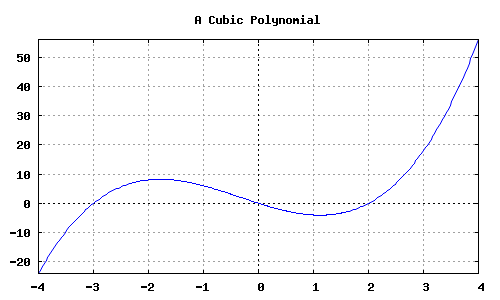
\includegraphics[width=3in]{example_1_1_1}



It appears that the function $P(x)$ has zeros at $x=-3$, $x=0$, and $x=2$.  We can verify these zeros by using wxMaxima to factor $P(x)$:

\begin{verbatim}
(%i3) factor(P);
(%o3) (x-2)*x*(x+3)
\end{verbatim}

Another option is to actually solve the equation $P(x)=0$:

\begin{verbatim}
(%i4) solve(P=0,x);
(%o4) [x=-3,x=2,x=0]
\end{verbatim}

\end{exmp}\

\line(1,0){60}
\linethickness{0.5mm}

\subsection{Rational Functions}

A \textbf{rational function} is a function of the form:

$$f(x)=\frac{P(x)}{Q(x)}$$

where $P(x)$ and $Q(x)$ are polynomials, and the domain is restricted to values of $x$ for which $Q(x){\neq}{0}$.  We are usually interested in finding zeros and asymptotes of rational functions.

\begin{exmp}
For the rational function $Q(x)=\frac{x^{2}-x-2}{2x^{2}-x-3}$, find all asymptotes, zeros and holes. Plot $Q(x)$ along with all asymptotes, zeros and holes. \\
${}$\\
If we don't indicate the $y$ range to wxMaxima, the vertical scale of this graph is too large for us to see the its essential features.  To fix the problem, we use \verb|xrange| and \verb|yrange| to explicitly define the window size.


\begin{verbatim}
(%i5) Q:(x^2-x-2)/(2*x^2-x-3);
(%o5) (x^2-x-2)/(2*x^2-x-3)

(%i6) wxdraw2d(
      xaxis=true,
      yaxis=true,
      grid=true,
      title="A Rational Function",
      xrange=[-10,10],
      yrange=[-10,10],
      explicit((Q),x,-10,10)
      );
\end{verbatim}

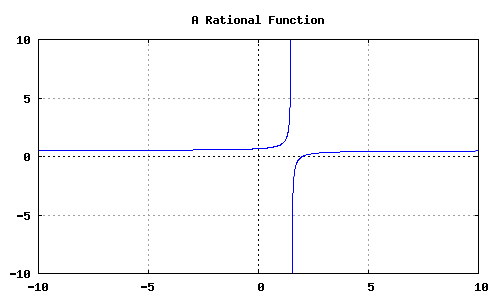
\includegraphics[width=3in]{example_1_1_2_1}



The graph has one zero, one vertical asymptote and one horizontal asymptote.  In order to find the exact values of these features we will have to factor the numerator and denominator of $Q(x)$ as far as possible.  The \verb|num| and \verb|denom| commands can extract the numerator and denominator of $Q(x)$ for factoring:

\begin{verbatim}
(%i7) factor(num(Q));
(%o7) (x-2)*(x+1)
(%i8) factor(denom(Q));
(%o8) (x+1)*(2*x-3)
\end{verbatim}

We notice that there is a common factor of $(x+1)$ that cancels out, but it can't be completely ignored!  Since the denominator of $Q(x)$ vanishes at $x=-1$, $Q(x)$ is undefined there.  We represent this as a hole in the graph; unfortunately wxMaxima does not make the hole visible, but we can represent the hole decently by inserting a circle at the point $(-1,0.6)$ in the graph.\\
${}$\\
With $Q(x)$ simplified to $\frac{x-2}{2x-3}$, we can quickly determine that the zero (where the numerator is zero) is at $x=2$ and the vertical asymptote (where the denominator is zero) has the equation $x=3/2$.  Of course, we can coax wxMaxima into doing the algebra for us if desired:

\begin{verbatim}
(%i9) R:ratsimp(Q);
(%o9) (x-2)/(2*x-3)
(%i10) solve(num(R)=0);
(%o10) [x=2]
(%i11) solve(denom(R)=0);
(%o11) [x=3/2]
\end{verbatim}

We determine the horizontal asymptote by using the \verb|limit| command in wxMaxima.  We will eventually study limits in much greater detail, but for now we just say that $\lim_{x \to \pm\infty} Q(x)=L$ indicates there is a horizontal asymptote $y=L$.  The limit simply means that ``$Q(x)$ gets close to $L$ as $x$ becomes `large' ''.\\
${}$\\
We compute the limits at infinity in wxMaxima and find that there is a horizontal asymptote at $y=1/2$.

\begin{verbatim}
(%i12) limit(Q,x,inf);
(%o12) 1/2
(%i13) limit(Q,x,-inf);
(%o13) 1/2
\end{verbatim}



Finally, we put all the information together in a single graph.  Note that the vertical asymptote $x=1.5$ must be defined \textit{parametrically} as discussed in Module 0.

\begin{verbatim}
(%i14) wxdraw2d(
       xaxis=true,
       yaxis=true,
       grid=true,
       title="A Rational Function",
       xrange=[-5,5],
       yrange=[-5,5],
       color=black,
         explicit((Q),x,-5,5),
       color=red,
       line_type=dots,
         explicit((0.5),x,-5,5),
         parametric(1.5,t,t,-5,5),
       point_type=6,
         points([[-1,0.6]]),
       point_type=7,
         points([[2,0]])
       ); 
\end{verbatim}

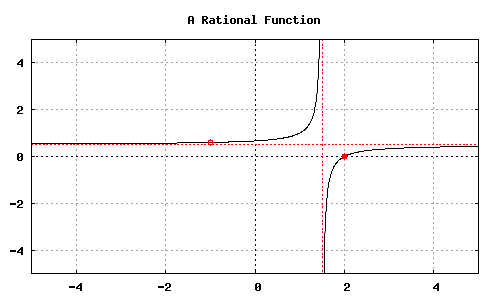
\includegraphics[width=3in]{example_1_1_2_2}



\end{exmp}
\line(1,0){60}
\linethickness{0.5mm}
\pagebreak

\section{Trigonometric Functions}\label{Trigonometric Functions}

\subsection{The Basic Trig Functions}

The basic trigonometric functions are defined as follows:\\
${}$\\
\hspace{4ex} $\sin{x}$ is the $y$-coordinate of a point on the unit circle at an angle of $x$.\\
${}$\\
  
\hspace{4ex} $\cos{x}$ is the $x$-coordinate of a point on the unit circle at an angle of $x$\\
${}$\\
  
\hspace{4ex} $\tan{x}$ is the ratio $\displaystyle \frac{\sin(x)}{\cos(x)}$\\
${}$\\
The angle, $x$, is measured in radians counterclockwise from the positive $x$-axis.

\begin{exmp}
Make a plot of the sine function on the interval $[0,4\pi]$.  Identify the period and the first three zeros (roots) of the sine function.\\

\begin{verbatim}
(%i1) S:sin(x)$
(%i2) wxdraw2d(
      xaxis=true,
      yaxis=true,
      grid=true,
      title="The Sine Function",
      xrange=[0,4*%pi],
      yrange=[-1.5,1.5],
      explicit((S),x,0,4*%pi)
      );
\end{verbatim}

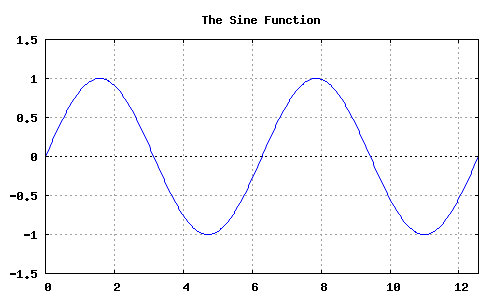
\includegraphics[width=3in]{example_1_2_1}

${}$\\

We see that the sine function is a simple wave with a period of $2\pi\approx6.3$.  The zeros of the function can be computed using \verb|"find_root"| -- unfortunately the command only gives us numerical approximations for one root at a time on a closed interval. We will have to eyeball the roots and construct closed intervals accordingly.  The first three roots are approximated as follows:

\begin{verbatim}
(%i3) find_root(S,0,1);
(%o3) 0.0
(%i4) find_root(S,2,4);
(%o4) 3.141592653589793
(%i5) find_root(S,6,8);
(%o5) 6.283185307179586
\end{verbatim}

We recognize that these are numerical approximations for ${0},{\pi},{2\pi},{\dots}$



\end{exmp}

\line(1,0){60}
\linethickness{0.5mm}

\begin{exmp}

Make a plot of the tangent function on the interval $[0,4\pi]$.  Identify the period, the zeros (roots) and the equations of the vertical asymptotes.\\


\begin{verbatim}
(%i6) T:tan(x)$
(%i7) wxdraw2d(
       xaxis=true,
       yaxis=true,
       grid=true,
       title="The Tangent Function",
       xrange=[0,4*%pi],
       yrange=[-8,8],
       explicit((T),x,0,4*%pi)
       );
 
\end{verbatim}

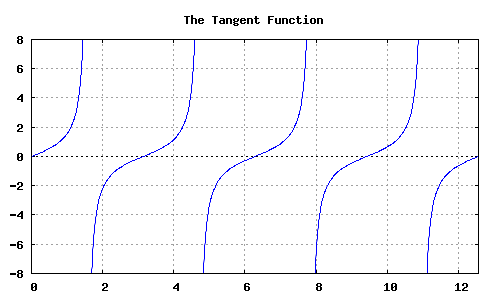
\includegraphics[width=3in]{example_1_2_2_1}

${}$\\

The tangent function has a period of only $\pi\approx3.14$.  The roots occur when the numerator $\sin{x}=0$, which we recall corresponds to $x={0},{\pi},{2\pi},{\dots}$.  The tangent function has many vertical asymptotes corresponding to the values of $x$ for which the denominator $\cos{x}=0$.  For this example, we will just recall that $\cos{x}=0$ when $x=\frac{\pi}{2},x=\frac{3\pi}{2},\dots$, which provides our list of equations for vertical asymptotes.\\

${}$\\

Replotting the function with vertical asymptotes, we obtain:\\

\begin{verbatim}
(%i8) wxdraw2d(
       xaxis=true,
       yaxis=true,
       grid=true,
       title="The Tangent Function",
       xrange=[0,4*%pi],
       yrange=[-8,8],
       color=black,
       explicit((T),x,0,4*%pi),
       color=red,
       line_type=dots,
         parametric(%pi/2,t,t,-8,8),
         parametric(3*%pi/2,t,t,-8,8),
         parametric(5*%pi/2,t,t,-8,8),
         parametric(7*%pi/2,t,t,-8,8)
       );
\end{verbatim}

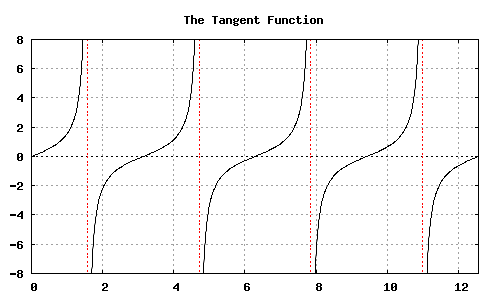
\includegraphics[width=3in]{example_1_2_2_2}


\end{exmp}

\line(1,0){60}
\linethickness{0.5mm}

\subsection{Graphs of Sinusoidal Functions}

A function of the form $f(x)=A\cos{(Bx+\phi)+C}$ or $f(x)=A\sin{(Bx+\phi)+C}$ is called \textbf{sinusoidal}.  The graph of a sinusoidal function is a simple wave.\\
${}$\\
The \textbf{midline} of a sinusoidal function is the line $y=C$: a horizontal line half-way between the minimum and maximum values.  \\
${}$\\
The \textbf{amplitude} of a sinusoidal function is given by $A$:  the distance from the midline to the maximum and minimum values of the function.\\
${}$\\
The \textbf{period} of a sinusoidal function is determined by $B$ by the formula $T=\frac{2\pi}{B}$. Period is the smallest horizontal distance covered before the sinusoidal function begins to repeat itself.\\
${}$\\
The \textbf{phase shift} of a sinusoidal function is given by $\phi$.  Phase shift is the \textit{fraction of a period shift} multiplied by $2\pi$, where a negative value corresponds to a rightward shift, and a postive value corresponds to a leftward shift.\\
${}$\\
\begin{exmp}

Plot $f(x)=\cos{x}$, $g(x)=\cos{x}+1$, and $h(x)=\cos{x}-2$ on the same graph using red, blue and black, respectively.  Include a key to identify each plot in the graph.\\


\begin{verbatim}
(%i9)  F:cos(x)$
       G:cos(x)+1$
       H:cos(x)-2$
(%i12) wxdraw2d(
       xaxis=true,
       yaxis=true,
       grid=true,
       title="Three Cosines With Different Midlines",
       key="y=cos(x)",
       color="red",
        explicit((F),x,-2*%pi,2*%pi),
       key="y=cos(x)+1",
       color="blue",
        explicit((G),x,-2*%pi,2*%pi),
       key="y=cos(x)-2",
       color="black",
       explicit((H),x,-2*%pi,2*%pi)
       );
\end{verbatim}

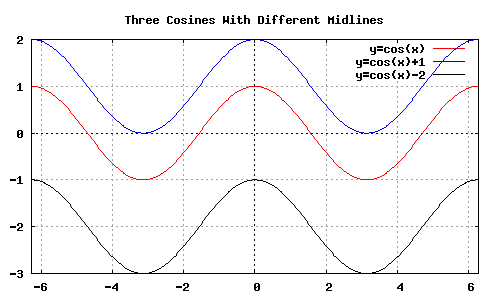
\includegraphics[width=3in]{example_1_2_3}

We see that the additive constant just shifts the midline up or down by the corresponding number of units.

\end{exmp}

\line(1,0){60}
\linethickness{0.5mm}




\begin{exmp}
Plot the three functions $f_1=\sin{x}$, $f_2=2\sin{x}$, and $f_3=3\sin{x}$ in red, blue and black, respectively.  Include a key to identify each plot in the graph.\\


\begin{verbatim}
(%i13) F1:sin(x)$
       F2:2*sin(x)$
       F3:3*sin(x)$
(%i16) wxdraw2d(
       xaxis=true,
       yaxis=true,
       grid=true,
       title="Three Sine Waves With Different Amplitudes",
       key="y=sin(x)",
       color=red,
         explicit((F1),x,0,4*%pi),
       key="y=2*sin(x)",
       color=blue,
         explicit((F2),x,0,4*%pi),
       key="y=3*sin(x)",
       color=black,
         explicit((F3),x,0,4*%pi)
       );
\end{verbatim}


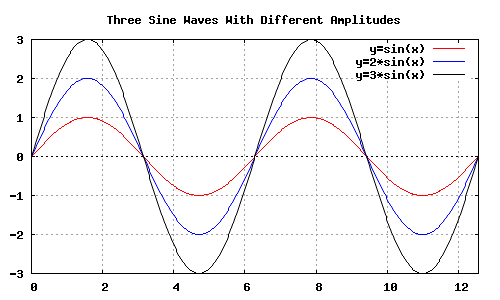
\includegraphics[width=3in]{example_1_2_4}





\end{exmp}

\line(1,0){60}
\linethickness{0.5mm}





\begin{exmp}

Plot $f(x)=\cos{x}$ and $g(x)=\cos{\pi x}$ on the same graph using black and red, respectively.  Include a key to identify each plot in the graph.  Note the periods of both functions and compare to the formula $T=\frac{2\pi}{B}$.\\


\begin{verbatim}
(%i17) F:cos(x)$
       G:cos(%pi*x)$
(%i19) wxdraw2d(
       xaxis=true,
       yaxis=true,
       grid=true,
       title="Two Cosines with Different Periods",
       key="y=cos(x)",
       color="black",
        explicit((F),x,-2*%pi,2*%pi),
       key="y=cos(%pi*x)",
       color="red",
       explicit((G),x,-2*%pi,2*%pi)
       );
\end{verbatim}

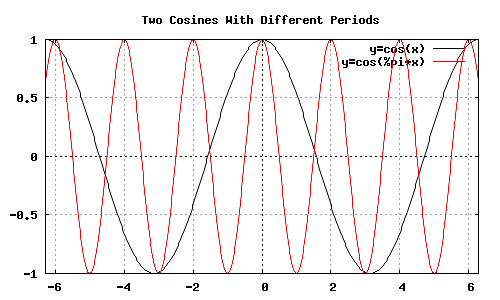
\includegraphics[width=3in]{example_1_2_5}

We see that the original cosine function $f(x)=\cos{x}$ has a period of $2\pi$ (a little more than 6), while the new function $g(x)=\cos{(\pi x)}$ has a period of exactly 2.  This agrees with the formula $T=\frac{2\pi}{B}=\frac{2\pi}{\pi}=2$.


\end{exmp}

\line(1,0){60}
\linethickness{0.5mm}




\pagebreak
\begin{exmp}

Plot $f(x)=\cos{(2\pi x)}$ and $g(x)=\cos{(2\pi x+\frac{\pi}{2})}$ on the same graph using black and red, respectively.  Include a key to identify each plot in the graph.  Note the periods of both functions and verify the definition of phase shift.\\


\begin{verbatim}
(%i20) F:cos(2*%pi*x)$
       G:cos(2*%pi*x+%pi/2)$
(%i22) wxdraw2d(
       xaxis=true,
       yaxis=true,
       grid=true,
       title="Two Cosines With Different Phase Shifts",
       key="y=cos(2*%pi*x)",
       color="black",
        explicit((F),x,-1,1),
       key="y=cos(2*%pi*x+%pi/2)",
       color="red",
        explicit((G),x,-1,1)
       );
\end{verbatim}

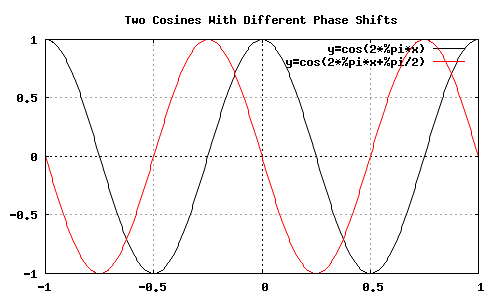
\includegraphics[width=3in]{example_1_2_6}

We see that $f(x)=\cos{(2\pi x)}$ is a cosine function with period 1, and $g(x)=\cos{(2\pi x+\frac{\pi}{2})}$ is a cosine function with period 1 that has been shifted to the left by $\frac{1}{4}$.  This agrees with the definition of phase shift, since $\frac{\pi}{2}$ is $\frac{1}{4}$ of $2\pi$: in this case a quarter of a period is simply $\frac{1}{4}$.


\end{exmp}

\line(1,0){60}
\linethickness{0.5mm}

\pagebreak



\section{Exponential Functions}\label{Exponential Functions}

An \textbf{exponential function} is a function of the form $f(x)=a\cdot b^x$ or $f(x)=a\cdot e^{kx}$.  We convert between the two forms by using the relation $k=\ln{b}$.\\
${}$\\
We are usually interested in the \textit{initial value} ($y$-intercept) and the \textit{growth rate} (as determined by $b$ or, equivalently, $k$). Simple exponential functions are asymptotic to the $x$-axis.\\
${}$\\
\begin{exmp}

The functions $f_1(x)=2^x$, $f_2(x)=2\cdot 2^x$ and $f_3(x)=3\cdot 2^x$ all have the same growth rate but different initial values.  Plot the functions in red, blue and black, respectively.  Include a key in your graph to indicate which function is which.\\

\begin{verbatim}
(%i1) F1:2^x$
      F2:2*2^x$
      F3:3*2^x$
(%i4) wxdraw2d(
       xaxis=true,
       yaxis=true,
       grid=true,
       xrange=[-3,3],
       yrange=[-1,20],
       title="Three Exponential Functions with Different Initial Values",
       key="y=2^x",
       color=red,
         explicit((F1),x,-3,3),
       key="y=2*2^x",
       color=blue,
         explicit((F2),x,-3,3),
       key="y=3*2^x",
       color=black,
         explicit((F3),x,-3,3)
       );
\end{verbatim}

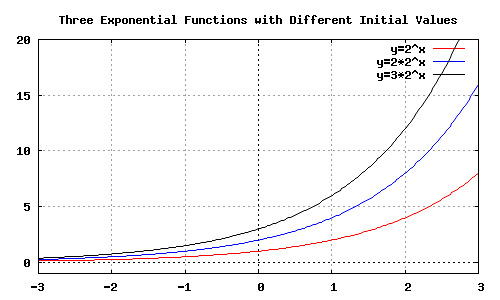
\includegraphics[width=3in]{example_1_3_1}

\end{exmp}

\line(1,0){60}
\linethickness{0.5mm}
\pagebreak

\begin{exmp}

The functions $f_1(x)=e^x$, $f_2(x)=e^{2x}$ and $f_3(x)=e^{3x}$ all have the same initial value but different growth rates.  Plot the functions in red, blue and black, respectively.  Include a key in your graph to indicate which function is which.\\

\begin{verbatim}
(%i5) F1:exp(x)$
      F2:exp(2*x)$
      F3:exp(3*x)$
(%i6) wxdraw2d(
       xaxis=true,
       yaxis=true,
       grid=true,
       xrange=[-3,3],
       yrange=[-1,20],
       title="Three Exponential Functions with Different Growth Rates",
       key="y=e^x",
       color=red,
         explicit((F1),x,-3,3),
       key="y=e^(2x)",
       color=blue,
         explicit((F2),x,-3,3),
       key="y=e^(3x)",
       color=black,
         explicit((F3),x,-3,3)
       );
\end{verbatim}

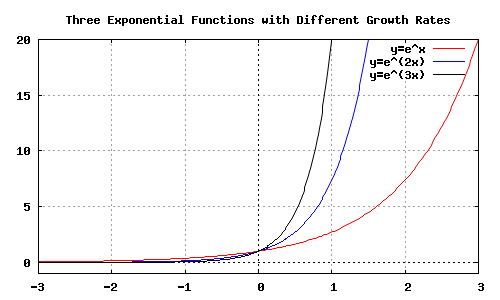
\includegraphics[width=3in]{example_1_3_2}

\end{exmp}

\line(1,0){60}
\linethickness{0.5mm}
\pagebreak

\section{Function Transformations}\label{Function Transformations}

\textit{Function transformations} are simple modifications of a function's formula which result in predictable changes to its graph. \\
${}$\\
Compared to $f(x)$,\\
${}$\\
 
\begin{tabular}{l l} 
\hspace{4ex} $g(x)=f(-x)$ & is reflected about the $y$-axis.\\
\hspace{4ex} $g(x)=-f(x)$ & is reflected about the $x$-axis.\\
\hspace{4ex} $g(x)=cf(x)$ & is stretched vertically by a factor of $c$.\\
\hspace{4ex} $g(x)=f(cx)$ & is compressed horizontally by a factor of $c$.\\
\hspace{4ex} $g(x)=f(x+c)$ & is shifted left by $c$ units.\\
\hspace{4ex} $g(x)=f(x)+c$ & is shifted up by $c$ units.\\
\end{tabular}

${}$\\

\begin{exmp}
Let $f(x)=e^{0.5\cdot x}$.  Use wxMaxima to find explicit formulas for $g(x)=f(-x)$, $h(x)=-f(x)$, $i(x)=f(x+5)$ and $j(x)=f(x)+5$.  Plot $f(x)$ in black and the transformations in blue, red, green and yellow, respectively.\\
${}$\\

When we want to use function properties in wxMaxima, we need to define a function (rather than an expression) by using \verb|`:='| instead of \verb|`:'|.\\

\begin{verbatim}
(%i1) F(x):=exp(0.5*x)$
(%i2) G(x):=F(-x)$
      H(x):=-F(x)$
      I(x):=F(x+5)$
      J(x):=F(x)+5$
(%i6) G(x);
(%o6) %e^(-0.5*x)
(%i7) H(x);
(%o7) -%e^(0.5*x)
(%i8) I(x);
(%o8) %e^(0.5*(x+5))
(%i9) J(x);
(%o9) %e^(0.5*x)+5
\end{verbatim}

We see that the formulas are given by $g(x)=e^{-.5x}$, $h(x)=-e^{0.5x}$, $i(x)=e^{0.5(x+5)}$, and $j(x)=e^{0.5x}+5$.  We plot the functions in a reasonable window size below:\\

\begin{verbatim}
(%i10) wxdraw2d(
      xaxis=true,
      yaxis=true,
      grid=true,
      title="Several Transformations of f(x)=exp(-0.5x)",
      xrange=[-10,10],
      yrange=[-10,10],
      color=black,
      key="f(x)",
       explicit((F(x)),x,-10,10),
      color=blue,
      key="g(x)=f(-x)",
       explicit((G(x)),x,-10,10),
      color=red,
      key="h(x)=-f(x)",
       explicit((H(x)),x,-10,10),
      color=green,
      key="f(x+5)",
       explicit((I(x)),x,-10,10),
      color=yellow,
      key="f(x)+5",
       explicit((J(x)),x,-10,10)
      );
\end{verbatim}

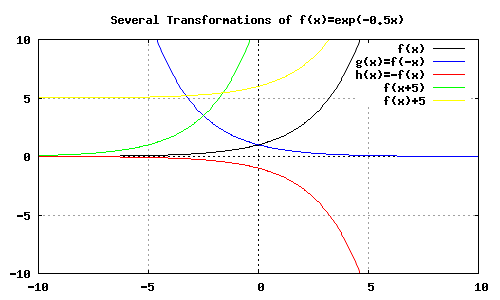
\includegraphics[width=3in]{example_1_4_1}

\end{exmp}

\line(1,0){60}
\linethickness{0.5mm}

${}$\\

The midline, amplitude, period and phase shift of a sinusoidal function can be viewed as arising from one or more function transformations on the sine or cosine functions.  The following example illustrates how a horizontal stretch/compression can change the \textit{period} of a sinusoid.

\begin{exmp}
Let $f(x)=\sin{x}$.  Plot $f(x)$ together with $g(x)=f(2x)$ with sensible color coding and a key.  Then plot $f(x)$ and $h(x)=f(0.5x)$ in a separate plot. Use the interval ${[{-4\pi},4\pi]}$ for both plots.  Comment on the periods of all three functions.\\

\begin{verbatim}
(%i11)F(x):=sin(x)$
      G(x):=F(2*x)$
      H(x):=F(0.5*x)$
(%i14) wxdraw2d(
       xaxis=true,
       yaxis=true,
       grid=true,
       title="Horizontal Stretch and Compression of y=sin(x)",
       key="f(x)",
       color=black,
        explicit((F(x)),x,-4*%pi,4*%pi),
       key="f(2x)",
       color=blue,
        explicit((G(x)),x,-4*%pi,4*%pi)
       );
\end{verbatim}

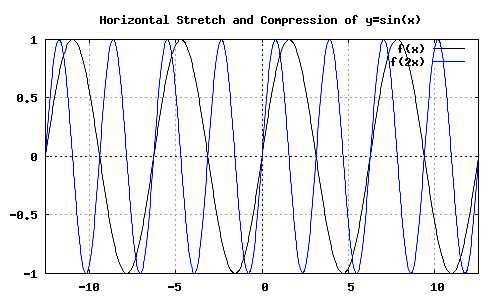
\includegraphics[width=3in]{example_1_4_2_1}

We see that $g(x)=f(2x)$ has half the period of the original function:  it has been compressed horizontally by a factor of 2 in agreement with the formula $T=\frac{2\pi}{B}$.

\begin{verbatim}
(%i15) wxdraw2d(
       xaxis=true,
       yaxis=true,
       grid=true,
       title="Horizontal Stretch and Compression of y=sin(x)",
       key="f(x)",
       color=black,
        explicit((F(x)),x,-4*%pi,4*%pi),
       key="f(0.5*x)",
       color=red,
        explicit((H(x)),x,-4*%pi,4*%pi)
       );
\end{verbatim}

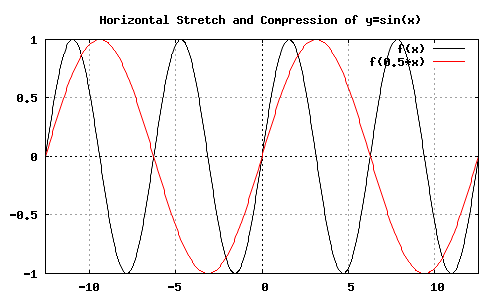
\includegraphics[width=3in]{example_1_4_2_2}

We see that $h(x)=f(0.5x)$ has twice the period of the original function:  it has been stretched horizontally by a factor of 2 in agreement with the formula $T=\frac{2\pi}{B}$.

\end{exmp}

\line(1,0){60}
\linethickness{0.5mm}


\pagebreak

\section{Parity of Functions}\label{Parity of Functions}

\textit{Parity} is used to refer in general to the ``evenness'' or ``oddness'' of a function.  The algebraic definitions are as follows:
$$f(x) \text{ is an even function if } f(-x)=f(x).$$
$$f(x) \text{ is an odd function if } f(-x)=-f(x).$$
It is important to realize that the algebraic definitions correspond to useful \textit{symmetries} in the graph of a function.  In terms of function transformations, we say that the graph of an even function is the same as the reflection about the $y$ axis, and the graph of an odd function is the same as the combined reflections of the graph about the $x$ and $y$ axes.   \\
${}$\\

\begin{exmp}
Use wxMaxima to verify algebraically that $f(x)=\frac{1}{x^2-4}$ is an even function.  Plot $f(x)$ and comment on the symmetry of the graph.\\

\begin{verbatim}
(%i1) f(x):=1/(x^2-4)$
(%i2) f(-x);
(%o2) 1/(x^2-4)
\end{verbatim}

We see that the formula for $f(x)$ is exactly the same as the formula for $f(-x)$, so the function is even.  Next, we produce a plot of $f(x)$ in a reasonable window:

\begin{verbatim}
(%i3) wxdraw2d(
      xaxis=true,
      yaxis=true,
      xrange=[-5,5],
      yrange=[-10,10],
      grid=true,
      title="An Even Rational Function",
      color=black,
      explicit((f(x)),x,-5,5)
      ); 
\end{verbatim}


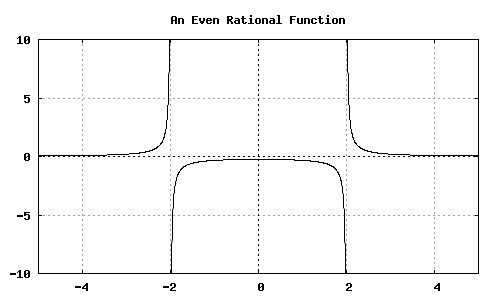
\includegraphics[width=3in]{example_2_1_1}

Like all even functions, the graph of $f(x)$ is symmetric about the $y$-axis.

\end{exmp}

\line(1,0){60}
\linethickness{0.5mm}

\pagebreak
\begin{exmp}
Use wxMaxima to verify algebraically that $f(x)=\sin{x}$ is an odd function.  Plot $f(x)$ and comment on the symmetry of the graph.\\

\begin{verbatim}
(%i4) f(x):=sin(x)$
(%i5) f(-x);
(%o5) -sin(x)
\end{verbatim}

We see that the formula for $f(-x)$ is $-\sin{x}$.  The function is odd because $f(-x)=-f(x)$.  

\begin{verbatim}
(%i6) wxdraw2d(
      xaxis=true,
      yaxis=true,
      xrange=[-5,5],
      yrange=[-2,2],
      grid=true,
      title="An Odd Trigonometric Function",
      color=black,
      explicit((f(x)),x,-5,5)
      );
\end{verbatim}

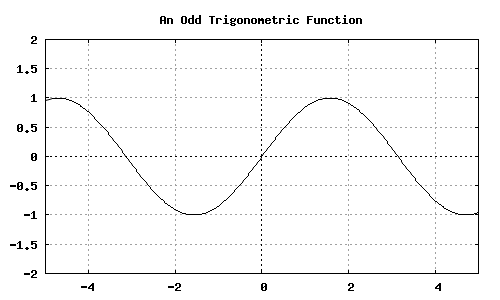
\includegraphics[width=3in]{example_2_1_2}

Like all odd functions, $f(x)=\sin{x}$ is ``symmetric about the origin''; i.e., a combination of reflections about the $x$ and $y$ axes yields the same graph.  The symmetry is equivalent to a $180^\circ$ rotational symmetry about the origin.

\end{exmp}

\line(1,0){60}
\linethickness{0.5mm}

\pagebreak

\section{Algebraic Combinations of Functions}\label{Algebraic Combinations of Functions}

Functions $f(x)$ and $g(x)$ can be algebraically combined in a variety of ways to produce a new function, $h(x)$:\\
  
\begin{align*}  
&\text{A sum or difference:  } & h(x)&=f(x) \pm g(x) \\
  \\
&\text{A linear combination: } & h(x)&=af(x)+bg(x)\\
  \\
&\text{A product:  } & h(x)&=f(x)g(x)=(f\cdot g)(x)\\
  \\
&\text{A quotient:  } & h(x)&=\frac{f(x)}{g(x)}, \text{ provided }g(x)\neq 0 
\end{align*}

To lie in the domain of a function combination, a value of $x$ must lie in the domain of both $f(x)$ and $g(x)$.  In all cases, the combination happens ``point-by-point''.

\begin{exmp}
Define $f(x)=4-x^2$ and $g(x)=x$, and $h(x)=f(x)+g(x)$.  Make a plot of all three functions, with $f(x)$ and $g(x)$ shown in grey and $h(x)$ shown in black.  In addition, plot the points $(1,f(1))$, $(1,g(1))$ and $(1,h(1))$ as solid circles and comment on the ``point-by-point'' addition of functions. \\

\begin{verbatim}
(%i1) f(x):=4-x^2$
      g(x):=x$
      h(x):=f(x)+g(x)$
(%i4) wxdraw2d(
      xaxis=true,
      yaxis=true,
      grid=true,
      title="Two Functions, f(x) and g(x) and Their Sum, h(x)",
      xrange=[-10,10],
      yrange=[-10,10],
      color=grey,
       key="f(x)",
         explicit((f(x)),x,-10,10),
       key="g(x)",
         explicit((g(x)),x,-10,10),
       key="h(x)",
       color=black,
         explicit((h(x)),x,-10,10),
       key="",
       color=red,
       point_type=7,
         points([[1,f(1)],[1,g(1)],[1,h(1)]])
       );
\end{verbatim}

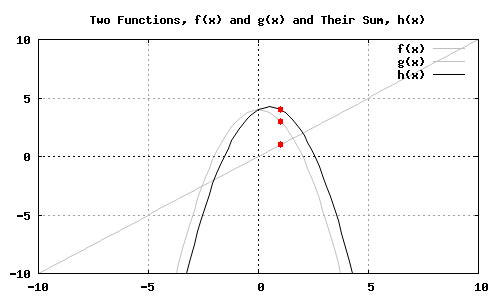
\includegraphics[width=3in]{example_2_2_1}

The highlighted points make it clear how function addition works: $f(1)=3$, $g(1)=1$, so $h(1)$ is just $3+1=4$.  It is always possible to quickly sketch sums, differences and so on by just looking at the plots of the participant functions point-by-point.

\end{exmp}

\line(1,0){60}
\linethickness{0.5mm}



\begin{exmp}

Define $f(x)=\sin{(\pi x)}$ and $g(x)=\cos{(\pi x)}-2$.  Now define $h(x)$ as a linear combination $h(x)=2f(x)+3g(x)$.  Make a plot of all three functions, with $f(x)$ and $g(x)$ shown in grey and $h(x)$ shown in black.  Comment on the period of each function.\\

\begin{verbatim}
(%i5) f(x):=sin(%pi*x)$
      g(x):=cos(%pi*x)-2$
      h(x):=f(x)+g(x)$
(%i8) wxdraw2d(
      xaxis=true,
      yaxis=true,
      grid=true,
      title="Two Functions, f(x) and g(x) and Their Sum, h(x)",
      xrange=[-4,4],
      yrange=[-6,6],
       color=grey,
       key="f(x)",
        explicit((f(x)),x,-4,4),
       key="g(x)",
        explicit((g(x)),x,-4,4),
       key="h(x)",
       color=black,
        explicit((h(x)),x,-4,4)
       ); 
\end{verbatim}

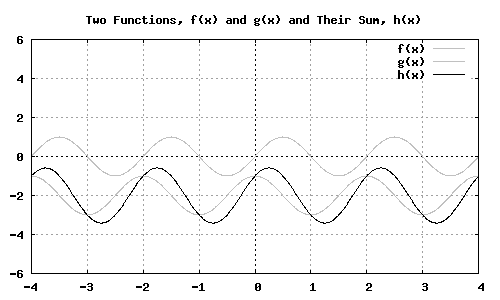
\includegraphics[width=3in]{example_2_2_2}

\end{exmp}

Remarkably, we see that the linear combination of two sinusoidal functions $f(x)$ and $g(x)$ (both of period 2) results in another sinusoidal function $h(x)$ (also with period 2).  As discussed in the Exercises, this only works if the participant functions have the same period.

\line(1,0){60}
\linethickness{0.5mm}



\begin{exmp}

Define functions $f(x)=e^{-0.4x}$, $g(x)=5\cos{(4 \pi x)}$, and $h(x)=f(x)\cdot g(x)$. Make a plot of all three functions, with $f(x)$ and $g(x)$ shown in grey and $h(x)$ shown in black.  How do the zeros of $h(x)$ compare to the zeros of $f(x)$ and $g(x)$?  \\ 

\begin{verbatim}
(%i9) f(x):=%e^(-0.4*x)$
      g(x):=5*cos(4*%pi*x)$
      h(x):=f(x)*g(x)$
(%i12)wxdraw2d(
      xaxis=true,
      yaxis=true,
      grid=true,
      title="Product of a Sinusoid and a Decaying Exponential",
      xrange=[0,10],
      yrange=[-5,5],
      color=grey,
       key="f(x)",
        explicit((f(x)),x,0,10),
       key="g(x)",
        explicit((g(x)),x,0,10),
       key="h(x)",
       color=black,
        explicit((h(x)),x,0,10)
       );
\end{verbatim}

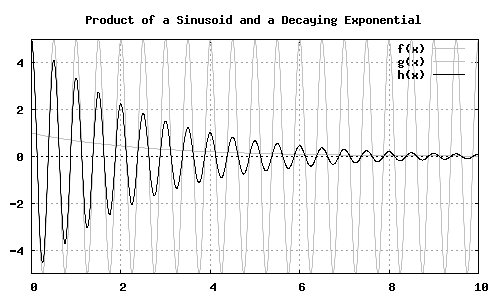
\includegraphics[width=3in]{example_2_2_3_1}

$f(x)$ is never zero, and $g(x)$ has many zeros occuring periodically.  Since $h(x)=f(x)\cdot g(x)$, it must vanish whenever $f(x)=0$ or $g(x)=0$, so it has exactly the same zeros as the cosine function.\\
${}$\\

We can refer to $h(x)$ as a ``sinusoidal function with a decaying amplitude''.  This type of function occurs frequently in physical applications. We notice that $g(x)$ repeatedly hits a minimum value of -5 and a maximum value of +5, and at these special points, $h(x)=\pm 5e^{-.4x}$.  If we plot these two functions $i(x)=5e^{-.4x}$ and $j(x)=-5e^{-.4x}$ they provide an upper and lower bound called an \textit{envelope}:

\begin{verbatim}
(%i13) i(x):=5*f(x)$
       j(x):=-5*f(x)$
(%i15) wxdraw2d(
      xaxis=true,
      yaxis=true,
      grid=true,
      title="Decaying Sinusoid With its Envelope",
      xrange=[0,10],
      yrange=[-5,5],
       color=black,
       key="5e^(-.4x)*cos(4pi*x)",
        explicit((h(x)),x,0,10),
       color=red, 
       key="Upper Bound",
        explicit((i(x)),x,0,10),
       key="Lower Bound",
        explicit((j(x)),x,0,10)
       );
\end{verbatim}

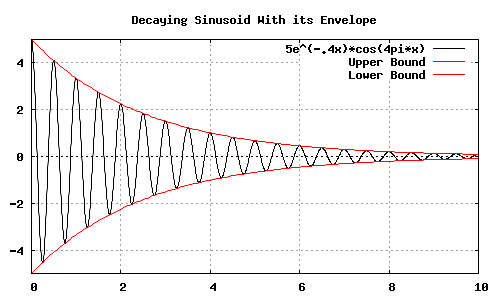
\includegraphics[width=3in]{example_2_2_3_2}

\end{exmp}

\line(1,0){60}
\linethickness{0.5mm}

\pagebreak

\section{Function Compositions}\label{Function Compositions}

A composition of two functions occurs when the output of one function is used as the input for another function.  Function compositions have a special notation:

\[(f\circ g)(x) = f(g(x))\]

Practically, this just means that we replace $x$ with $g(x)$ in the formula for $f(x)$.\\

${}$\\
\begin{exmp}
For the functions $f(x)=2x+1$ and $g(x)=\sqrt{x}$, use wxMaxima to compute $(f\circ g)(x)$ and $(g\circ f)(x)$.  Compute $(f\circ g)(-0.3)$ and $(g\circ f)(-0.3)$ and comment on the results.\\

\begin{verbatim}
(%i1) f(x):=2*x+1$
      g(x):=sqrt(x)$
(%i3) f(g(x));
(%o3) 2*sqrt(x)+1
(%i4) g(f(x));
(%o4) sqrt(2*x+1)
\end{verbatim}

We see that the formulas are different:  $(f\circ g)(x)=2\sqrt{x}+1$ while $(g\circ f)(x)=\sqrt{2x+1}$.  Now we check the compositions at $x=-0.3$:

\begin{verbatim}
(%i5) f(g(-0.3));
(%o5) 1.095445115010332*%i+1
(%i6) g(f(-0.3));
(%o6) 0.63245553203368
\end{verbatim}

$(f\circ g)(-0.3)$ is \textit{complex} because we evaluated a square root at a negative argument, while  $(g\circ f)(-0.3)$ does not have the same problem.  This is a good reminder that the domain of a composition must be evaluated carefully.  If desired, we can find the domain of each composition by determining the values of $x$ which correspond to non-negative numbers within the square root sign.

\end{exmp}

\line(1,0){60}
\linethickness{0.5mm}

${}$\\
 

\begin{exmp}

Express each of the following functions $i(x)$ as a composition of two or three simpler functions $f(x)$, $g(x)$ and possibly $h(x)$.  In each case, use wxMaxima to verify that $(f \circ g)(x)=i(x)$ or $(f \circ g \circ h)(x)=i(x)$

\begin{align*}  
&\text{a.  } i(x)=2e^{3x^2+1}  &\text{b.  } i(x)=\frac{1}{\tan{\sqrt{x}}}
\end{align*}

${}$\\

For part a., we see that $i(x)$ is just like $2e^x$ except the $x$ has been replaced by $3x^2+1$.  Thus, $g(x)=3x^2+1$ and $f(x)=2e^x$.  Checking with wxMaxima, we obtain:\\

\begin{verbatim}
(%i7) f(x):=2*%e^x$
      g(x):=3*x^2+1$
      i(x):=f(g(x))$
(%i8) i(x);
(%o8) 2*%e^(3*x^2+1)
\end{verbatim}

For part b., we see that $\tan{\sqrt{x}}$ is already a composition of two functions, then a third function $f(x)=\frac{1}{x}$ is required to get the reciprocal:\\

\begin{verbatim}
(%i9) f(x):=1/x$
      g(x):=tan(x)$
      h(x):=sqrt(x)$
      i(x):=f(g(h(x)))$
(%i10) i(x);
\end{verbatim}
\verb|(%o10)  | $\frac{1}{\tan{\sqrt{x}}}$

\end{exmp}

\line(1,0){60}
\linethickness{0.5mm}

\pagebreak

\section{Function Inverses}\label{Function Inverses}

We often use $x$ to indicate a domain element, $y$ to indicate a range element and $y=f(x)$ to indicate a rule connecting domain elements to range elements.  In order to be a \textit{function}, this rule must connect each domain element to only one range element (this is sometimes called the ``vertical line test'').\\
${}$\\
A function is called \textit{one-to-one} if each range element is connected to only one domain element; i.e., each $y$ is connected to only one $x$.   If a function is one-to-one, an \textit{inverse function} can be defined which takes the original range elements as ``inputs'' and delivers the original domain elements as ``outputs''.  If we solve the original equation $y=f(x)$ for $x$, then we automatially obtain a formula for the inverse function (as a function of $y$), and the notation for this function is $f^{-1}$:

$$\text{If } y=f(x)\text{, then }x=f^{-1}(y).$$
${}$\\
It is always true that $f^{-1}(f(x))=x$ and $f(f^{-1}(y))=y$.\\
${}$\\

In the case that a function is \textit{not} one-to-one, it might be useful to introduce a \textit{domain restriction} to force the function to be one-to-one.  That is, we remove $x$ values from the domain until each $y$ value is connected to only one $x$ value.  For example, the basic trigonometric functions have ``agreed upon'' domain restrictions in order to make them invertible.  This convenience comes at a price:  sometimes we have to think carefully about which $x$ value we are really trying to obtain when applying an inverse trigonometric function, and we may have to ``manually'' convert to an $x$ value outside the restricted domain.\\
${}$\\
Sometimes we wish to plot $f^{-1}$ as a function of $x$ instead of $y$; that is, we plot $y=f^{-1}(x)$.  By making this notational change, we are calling the ``original'' range elements of our function ``$x$'' instead of ``$y$'', and we are calling the ``original'' domain elements of our function ``$y$'' instead of ``$x$''.  As a consequence, every ordered pair in the graph of $f^{-1}(x)$ has its coordinates ``swapped'' when compared to the graph of $f(x)$.  The coordinate swap amounts to a reflection of $f(x)$ about the line $y=x$.  

${}$\\

\begin{exmp}
Define the function $f(x)=x^3$ in wxMaxima and use a graph to establish that the function is one-to-one.  Solve $y=x^3$  for $x$ in order to find the formula for $f^{-1}(y)$, then define $f^{-1}(x)$ as a new function in wxMaxima.  Verify that the compositions $f \circ f^{-1}$ and $f^{-1} \circ f$ behave properly.  Finally, make a plot of $f(x)$, $f^{-1}(x)$ and $y=x$ to verify that the $f^{-1}(x)$ is a reflection of $f(x)$ about $y=x$.\\

\begin{verbatim}
(%i1) F(x):=x^3$
(%i2) wxdraw2d(
      xaxis=true,
      yaxis=true,
      grid=true,
      title="y=x^3",
      explicit((F(x)),x,-2,2)
      ); 
\end{verbatim}
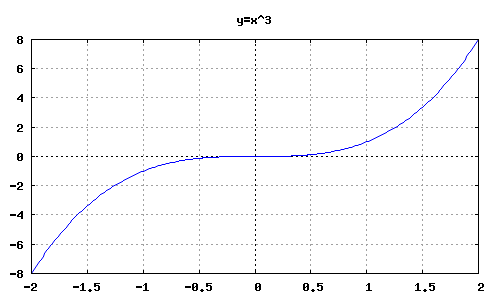
\includegraphics[width=3in]{example_2_4_1_1}

We can see that the function is one-to-one because each value of $y$ is connected to only one value of $x$.  Another way to say it is that any horizontal line only crosses the graph at one point.  Now we use wxMaxima to find a formula for the inverse:

\begin{verbatim}
(%i3) F:y=x^3$
(%i4) solve(F,x);
(%o4) [x=((sqrt(3)*%i-1)*y^(1/3))/2,x=-((sqrt(3)*%i+1)*y^(1/3))/2,x=y^(1/3)]
\end{verbatim}

wxMaxima finds three solutions for x, but we can ignore the complex solutions.  We see that the real solution is $x=\sqrt[3]{y}$, so $f^{-1}$ is the cubed root function.  Next, we can verify that the compositions of $f$ and $f^{-1}$ work as promised:

\begin{verbatim}
(%i5) F(x):=x^3$
      Finv(y):=y^(1/3)$
(%i6) F(Finv(y));
(%o6) y
(%i7) Finv(F(x));
(%o7) x
\end{verbatim}

It was not strictly necessary to define $f^{-1}$ as a function of $y$, but it is a good reminder that the inverse function operates on range elements of $f$.  Finally, we produce the plot (note the use of the \verb|dimensions| attribute to make it square for better illustration of the reflection):

\begin{verbatim}
(%i8) wxdraw2d(
       dimensions=[600,600],
       xaxis=true,
       yaxis=true,
       xrange=[-8,8],
       yrange=[-8,8],
       grid=true,
       title="y=x^3 and its Inverse",
       color=black,
        explicit((F(x)),x,-8,8),
       color=grey,
        explicit((Finv(x)),x,-8,8),
       color=red,
       line_type=dots,
        explicit((x),x,-8,8)
       );
\end{verbatim}


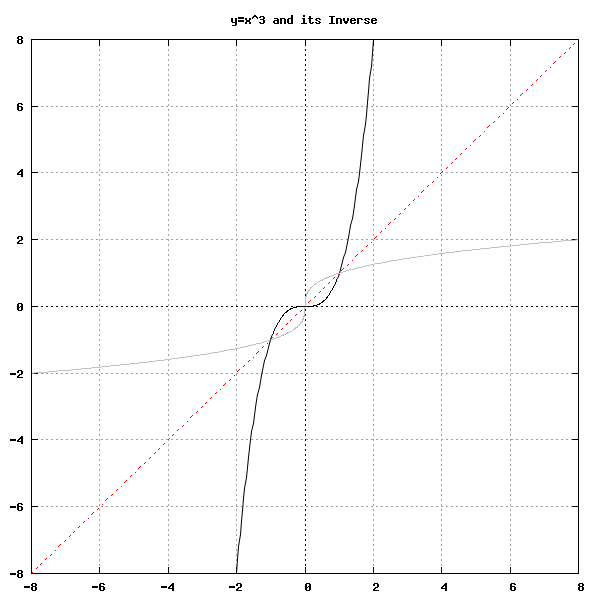
\includegraphics[width=3in]{example_2_4_1_2}


We see that $f$ and $f^{-1}$ are reflections about the line $y=x$ as expected.

\end{exmp}

\line(1,0){60}
\linethickness{0.5mm}


\begin{exmp}

Define $f(x)=\sin{x}$.  Plot $f(x)$ together with $y=0.9$.  How many times do these curves intersect?  What does this imply about the invertibility of $f(x)$?  Find decimal approximations for at least two of the intersections.  Now produce the same plot with $f(x)=\sin{x}$ restricted to the ``agreed-upon'' domain $[-\frac{\pi}{2},\frac{\pi}{2}]$ .  Comment on the invertibility of the resulting function.  Use wxMaxima to find a formula for the inverse function, then plot this function together with the restricted $f(x)$.  \\

\begin{verbatim}
(%i9) f(x):=sin(x)$
(%i10) wxdraw2d(
       xaxis=true,
       yaxis=true,
       xrange=[-2*%pi,2*%pi],
       yrange=[-1.5,1.5],
       grid=true,
       title="y=sin(x) and y=0.9",
       color=black,
        explicit((f(x)),x,-2*%pi,2*%pi),
       line_type=dots,
       explicit(0.9,x,-2*%pi,2*%pi)
       ); 
\end{verbatim}

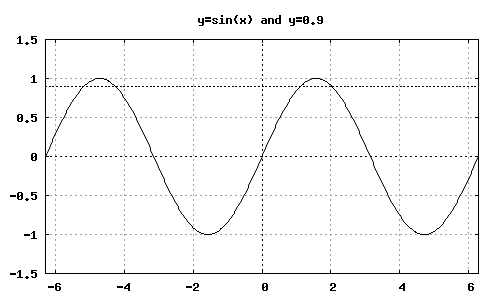
\includegraphics[width=3in]{example_2_4_2_1}

We see that the graphs intersect in several places (in fact, there are infinitely many intersections).  There are many $x$ values connected to the single $y$ value $0.9$, so $f(x)$ is not one-to-one, therefore not invertible.  Of course, this is true for all the other values in the range as well.  \\
${}$\\
We can find approximations to the two intersections on $[0,3]$ by using wxMaxima to solve on an interval.  We use \verb|find_root| to find the \textit{zeros} of the function $\sin(x)-0.9$.  Wherever this function is zero, we have a solution to $\sin(x)=0.9$.  We have to eyeball an interval for each intersection, making sure to capture only one intersection on each interval:

\begin{verbatim}
(%i11) find_root(sin(x)-0.9,0,1.9);
(%o11) 1.119769514998634
(%i12) find_root(sin(x)-0.9,1.9,3);
(%o12) 2.021823138591159
\end{verbatim}

We reproduce the same plot with the standard domain restriction for the sine function:

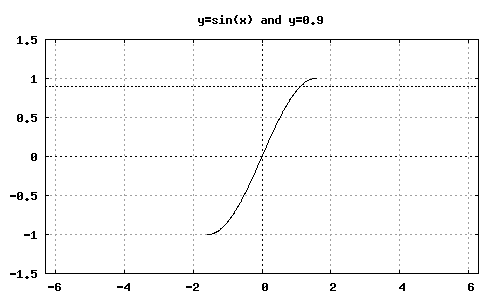
\includegraphics[width=3in]{example_2_4_2_2}

With the domain restriction to $[-\frac{\pi}{2},\frac{\pi}{2}]$, we see that each $y$ value of $f(x)$ is covered exactly once, so the restricted function is one-to-one, therefore invertible.  In particular, there is only one $x$ value for which $\sin(x)=0.9$. \\
${}$\\
Now we use wxMaxima to solve for $f^{-1}(y)$:

\begin{verbatim}
(%i13) solve(y=f(x),x);
       solve: using arc-trig functions to get a solution.
       Some solutions will be lost.
(%o14) [x=asin(y)]
\end{verbatim} 

wxMaxima is telling us that $f^{-1}(y)=\sin^{-1}{y}$.  \verb|asin| is wxMaxima's notation for $\arcsin$ (a synonym for $\sin^{-1}$).  wxMaxima has also pointed out that ``some solutions will be lost'' due to the implied domain restriction of the inverse sine function.\\
${}$\\
Finally, we can plot the restricted function $f(x)$ together with its inverse to observe the expected symmetry:

\begin{verbatim}
(%i15) wxdraw2d(
       dimensions=[600,600],
       xaxis=true,
       yaxis=true,
       xrange=[-1.6,1.6],
       yrange=[-1.6,1.6],
       grid=true,
       title="y=sin(x) (restricted to [-pi/2,pi/2]) its inverse",
       color=black,
        explicit((f(x)),x,-%pi/2,%pi/2),
       line_type=dots,
       explicit(asin(x),x,-1,1)
       );
\end{verbatim}

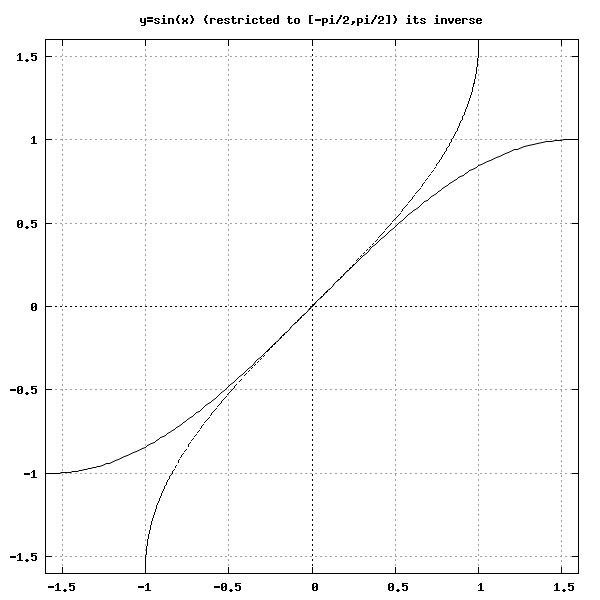
\includegraphics[width=3in]{example_2_4_2_3}

Again, we observe the symmetry about the line $y=x$.


\end{exmp}

\line(1,0){60}
\linethickness{0.5mm}


\begin{exmp}

Like the sine function, the standard domain restriction for the tangent function is $[-\frac{\pi}{2},\frac{\pi}{2}]$.  Solve the equation $\tan{x}=0.5$ by applying the inverse tangent function, subject to the condition that $x$ is somewhere on the interval $[\pi,2\pi]$.  In order to find the correct value of $x$, you will have to use the periodicity of the tangent function to ``manually'' convert the answer given by the inverse tangent function.  Make a plot of $y=\tan{x}$ and $y=0.5$ to illustrate the relationship between the two values of $x$.  \\
${}$\\

We begin by simply using wxMaxima's \verb|atan| command to solve the equation (an alternative is to use \verb|find_root| as we did in the last example):

\begin{verbatim}
(%i16) atan(0.5);
(%o16) 0.46364760900081
\end{verbatim}

This is certainly \textit{not} on the interval $[\pi,2\pi]$, so we need to ``manually'' find the desired solution.  To get a sense for where the solution may be, we make a plot of $y=\tan{x}$ and $y=0.5$ and look for intersections:

\begin{verbatim}
(%i17) wxdraw2d(
       xaxis=true,
       yaxis=true,
       yrange=[-2,2],
       xrange=[-6,6],
       grid=true,
       title="y=tan(x) and y=0.5",
       color=black,
        explicit((tan(x)),x,-6,6),
       color=red,
        explicit(0.5,x,-6,6)
       );
\end{verbatim}

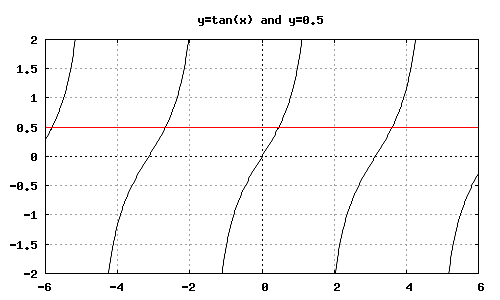
\includegraphics[width=3in]{example_2_4_3}

We see that the locations of all the intersections occur with the same periodicity of the tangent function itself.  To find the desired solution, we simply add $\pi$ to the previous solution.  To get a decimal approximation we use the \verb|float| command, and to check our answer we evaluate the tangent function once again (recall that \verb|%| means ``previous output''):

\begin{verbatim}
(%i18) atan(0.5)+%pi;
(%o18) %pi+0.46364760900081
(%i19) float(%);
(%o19) 3.605240262590599
(%i20) tan(%);
(%o20) 0.5
\end{verbatim}




\end{exmp}

\line(1,0){60}
\linethickness{0.5mm}

\pagebreak

\section{Module 1 Exercises}\label{Exercises}


\begin{enumerate}

\item
Plot the rational function $f(x)=\frac{x^2-2x+1}{3x^3-2}$ together with all horizontal and vertical asymptotes (use \verb|limit| to identify the horizontal asymptote).  Remember that the vertical asymptote must be defined \textit{parametrically} as shown in Example 1.1.2. \\
${}$\\
Note: When you algebraically search for the vertical asymptote, you will find some extraneous solutions (complex numbers), but the \textit{real} solution will also be included in the list.

\item  
Plot a sine function with period $\pi$, amplitude $2.5$, midline $y=1.5$ with a positive (leftward) phase shift equal to $1/3$ the period.  

\item
Plot $f(x)=\cos{x}$ on $[0,4\pi]$ and use \verb|find_root| to find decimal approximations to all the roots on this interval.  What are the \textit{exact} values of the roots?

\item
Plot the functions $f(x)=e^x$, $g(x)=x^e$ and $h(x)=x^x$ on the interval $[0,4]$.  Which function grows the fastest in the long-run?  The slowest?  Without doing any calculations, write down the intersection point for the three graphs.

\item
What minimum positive phase shift is required to transform a simple sine function into a cosine function?  Once you have chosen this value of $\phi$, make a plot of $f(x)=\sin{(x+\phi)}$ to verify that the cosine function is obtained.

\item
The trigonometric functions $\sec{x}$, $\csc{x}$ and $\cot{x}$ are defined as reciprocals of the basic trigonometric functions:

\verb|     |  $\sec{x}=\displaystyle \frac{1}{\cos{x}}$
\verb|     |  $\csc{x}=\displaystyle \frac{1}{\sin{x}}$
\verb|     |  $\cot{x}=\displaystyle \frac{1}{\tan{x}}$



Make three different plots to explore the relationship between each function and its reciprocal.  Each plot should contain the basic trigonometric function ($\sin$, $\cos$ or $\tan$) as a dotted red line and the reciprocal function ($\csc$, $\sec$ or $\cot$) as a solid black line.  Comment on the relationship between the zeros of one function and the vertical asymptotes of the other.



\item
Define the function $f(x)=x^2-5x$.  Define $g_1(x)=f(-x)$ and $h_1(x)=g_1(x+3)$; that is, perform a horizontal reflection followed by a horizontal shift.  Plot all three of these functions in the same window.

Now define $g_2(x)=f(x+3)$ and $h_2(x)=g_2(-x)$; that is, perform the same horizontal shift \textit{before} the same horizontal reflection.  Plot all three of these functions in the same window.

Comment on the importance of \textit{order} for the two transformations.

\item
Using the same function $f(x)$ as the last exercise, define $g_1(x)=2f(x)$ and $h_1(x)=g_1(-x)$ and make a plot of all three functions in the same window.

Now define $g_2(x)=f(-x)$ and $h_2(x)=2g_2(x)$ and make a plot of all three functions in the same window.

Does the order of the transformations matter in this case?  When do you think order matters, in general?


\item
Verify algebraically that $f(x)=e^{-x^2}$ is an even function.  Make a plot of $f(x)$ and verify that it has the correct symmetry.

\item
Define $f(x)=x^3$ and $g(x)=x^2+2x-3$ and $h(x)=\frac{f(x)}{g(x)}$.  Use wxMaxima to identify the values of $x$ that are not in the domain of $h(x)$.  Plot the function $h(x)$ together with the vertical asymptotes.

\item
Define $f(x)=e^{-0.1x^2}$ and $g(x)=4\cos{3 \pi x}$.  Plot $h(x)=f(x)\cdot g(x)$ along with the two functions that form the \textit{envelope}, as in Example 1.6.3.  Show $h(x)$ in black and the envelope in red lines.  Choose a window that clearly illustrates why $h(x)$ is sometimes called a ``wave packet''.

\item
The natural log function, $\ln{x}$ is the inverse of the natural exponential function $e^{x}$.  Algebraically verify that these two functions are inverses, then make a plot of both functions along with the line $y=x$.

\item
Find decimal approximations for all solutions to $\cos{x}=0.7$ on $[0,2\pi]$.  Include a plot that shows all the solutions as the intersections of two curves.  Finally, use the inverse cosine function to solve the equation, then figure out how to ``manually'' obtain the second solution from the first (it is \textit{not} as simple as shifting the solution by one period!).  Note:  the ``agreed-upon'' domain restriction for the cosine function is $[0,\pi]$.

\item
Find decimal approximations for the intersections of the inverse tangent function $\tan^{-1}(x)$ and the unit circle.  Hint:  the unit circle will have to be broken into two semi-circles (the upper and lower half) in order to pass the ``vertical line test''.  Make a plot showing the intersections.

\item
Any function $f(x)$ can be decomposed into even and odd parts by using the fact that $f(x)=\frac{1}{2}[f(x)+f(-x)]+\frac{1}{2}[f(x)-f(-x)]$ (the first term is even and the second is odd).  Define the function $f(x)=e^{x}$ and define $E(x)=\frac{1}{2}[f(x)+f(-x)]$ and $O(x)=\frac{1}{2}[f(x)-f(-x)]$.  Verify algebraically that $E(x)$ is even and $O(x)$ is odd.  Finally, produce plots of $E(x)$ and $O(x)$ to verify that they have the correct symmetry.  $E(x)$ and $O(x)$ actually have special names -- do a little research and write down the names of these special functions. 
 
\item
As discussed in Example 1.6.2, a linear combination of two sinusoidal functions with the same period results in another sinusoidal function with the same period.  If we combine two sinusoidal functions with \textit{different} periods, the result is no longer sinusoidal.  Define $f(x)=\sin{4x}$,  $g(x)=\cos{x}$, and $h(x)=3f(x)-g(x)$.  Plot the three functions with $h(x)$ shown in black and the others shown in grey.  What are the periods of $f(x)$ and $g(x)$?  What is the period of $h(x)$?  

\item
Based on the last exercise, formulate a general rule to predict the period of a linear combination of sinusoidal functions.  Does your rule work for the functions $f(x)=\sin{2x}$ and $g(x)=\sin{3x}$?  Produce a plot to test your rule, then adjust the rule if necessary.

\item
Using the interval $[0,4]$, find a function composition that results in a wave that ``wiggles'' faster as $x$ gets larger.  Make a nice plot of your function.


\end{enumerate}



\pagebreak

\chapter{Limits}

\vspace*{\fill}

\minitoc

\vspace*{\fill}


\flushleft{\textbf{\Large Key Commands Included in This Module}}
\newline
\newline

\begin{tabular}{l l l}
 \verb|for-do   |   &\verb|divide   |   &\verb|plus   |   \\
 \verb|print   |   &\verb|find_root   |   &\verb|   |   \\
 \verb|wxdraw2d   |   &\verb|inf   |   &\verb|   |   \\
 \verb|float   |   &\verb|minf   |   &\verb|   |   \\
 \verb|limit   |   &\verb|minus   |   &\verb|   |   \\
\end{tabular}



\pagebreak

\section{Using Sequences to Approximate Limits}\label{Using Sequences to Approximate Limits}

The informal definitions of \textbf{limits} are given as follows:\\
${}$\\
$\lim_{x \to a} f(x)=L$ means ``$f(x)$ becomes arbitrarily close to $L$ as $x$ becomes arbitrarily close to $a$.''\\
${}$\\
$\lim_{x \to a^{\pm}} f(x)=L$ means ``$f(x)$ becomes arbitrarily close to $L$ as $x$ becomes arbitrarily close to $a$ from the right/left (that is, for $x>a$ or $x<a$).''\\
${}$\\
$\lim_{x \to a^{\pm}} f(x)=\pm \infty$ means ``$f(x)$ becomes arbitrarily large and positive/negative as $x$ becomes arbitrarily close to $a$ from the right/left.''\\
${}$\\
$\lim_{x \to \pm\infty} f(x)=L$ means ``$f(x)$ becomes arbitrarily close to $L$ as $x$ becomes arbitrarily large and positive/negative''\\
${}$\\
We can explore these ideas numerically by using wxMaxima to evaluate $f(x)$ for a sequence of $x$-values that becomes closer and closer to the value of interest.  In the following examples, we use \verb|for-do| loops (also called simply ``do-loops'') to generate the sequences of $x$ and $f(x)$ values and print the results in tabular form.  Several types of sequences are illustrated, but the most important thing is that $x$ approaches the value of interest.

\begin{exmp}

Define $f(x)=\frac{1}{x^2}$, then evaluate each of the following limits by using a do-loop to generate an appropriate sequence of ordered pairs.  Produce a plot of $f(x)$ and comment on how it relates to the limits you have computed.\\
${}$\\
 
\verb|       |$\text{a.  } \lim_{x \to 0^{+}}f(x)$ 
\verb|          |$\text{b.  } \lim_{x \to 2^{-}}f(x)$  
\verb|          |$\text{c.  } \lim_{x \to +\infty}f(x)$\\

${}$\\
a. For this limit, we will use the sequence of $x$ values $.1,.01,.001,\dots,10^{-10}$.  Note how the do-loop is constructed to yield this sequence:  a formula is defined as $\frac{1}{10^i}$, then we run $i$ from 1 through 10. There are some extra quotation marks and commas used to create extra spaces in the printout.  Although wxMaxima doesn't make a nice table for us, the results are at least readable:

\begin{verbatim}
(%i1)  F(x):=1/(x^2)$
(%i2)  (print("x "," "," "," f"),
         for i:1 thru 10 do
         (x: 1/(10^i),
          f: F(x),
          print(x,"","",f))
        );
\end{verbatim}
\pagebreak
\begin{verbatim}     
 x     f
1/10  100
1/100  10000
1/1000  1000000
1/10000  100000000
1/100000  10000000000
1/1000000  1000000000000
1/10000000  100000000000000
1/100000000  10000000000000000
1/1000000000  1000000000000000000
1/10000000000  100000000000000000000
(%o2) done
\end{verbatim}

It appears that $f(x)$ is growing without bound as $x$ approaches 0 from the right, so we conclude that $\lim_{x \to 0^{+}}f(x)=\infty$ \\
${}$\\
b. For this limit, we use the sequence $1.9,1.99,\dots,1.9999999999$, which is obtained using the formula $2-\frac{1}{10^i}$.  We also use \verb|float| to tell wxMaxima to give us decimal approximations (otherwise the exact fraction output makes it hard to see what's going on):

\begin{verbatim}
(%i3) (print("x "," "," "," f"),
        for i:1 thru 10 do
        (x: float(2-1/(10^i)),
         f: float(F(x)),
         print(x,"","",f))
      );
     
 x    f
1.9  0.27700831024931
1.99  0.25251887578596
1.999  0.25025018762508
1.9999  0.25002500187513
1.99999  0.25000250001875
1.999999  0.25000025000019
1.9999999  0.250000025
1.99999999  0.2500000025
1.999999999  0.25000000025
1.9999999999  0.250000000025
(%o3) done
\end{verbatim}

We see that $f(x)$ is getting closer and closer to $0.25=\frac{1}{4}$ as $x$ gets closer and closer to $2$ from the left.  We conclude that $\lim_{x \to 2^{-}}f(x)=\frac{1}{4}$.\\
${}$\\


c.  For this limit, we will use the sequence $10,100,\dots,10^{10}$, which is obtained using the formula $10^i$:

\begin{verbatim}
(%i4) (print("x "," "," "," f"),
       for i:1 thru 10 do
        (x:(10^i),
         f: float(F(x)),
         print(x,"","",f))
       );
x  f
10  0.01
100  1.0*10^-4
1000  9.9999999999999995*10^-7
10000  1.0*10^-8
100000  1.0*10^-10
1000000  9.9999999999999998*10^-13
10000000  1.0*10^-14
100000000  9.9999999999999998*10^-17
1000000000  1.0000000000000001*10^-18
10000000000  9.9999999999999995*10^-21
(%o4) done
\end{verbatim}

We see that $f(x)$ gets very small as $x$ gets large and positive, so we conclude that $\lim_{x \to \infty}f(x)=0$.\\
${}$\\
Finally, we graph the function $f(x)=\frac{1}{x^2}$:

\begin{verbatim}
(%i5) wxdraw2d(
      xaxis=true,
      yaxis=true,
      grid=true,
      xrange=[-10,10],
      yrange=[-1,9],
      title="f(x)=1/x^2",
      color=black,
      explicit((F(x)),x,-10,10)
      );
\end{verbatim}

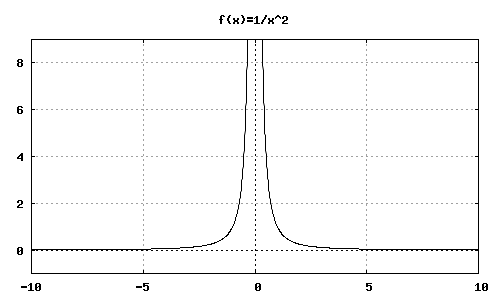
\includegraphics[width=3in]{example_3_1_1}

We see that $f(x)$ grows without bound as $x$ approaches zero from the right, $f(x)$ approaches $\frac{1}{4}$ as $x$ approaches 2 from the left and $f(x)$ approaches 0 as $x$ grows large and positive.

\end{exmp}

\line(1,0){60}
\linethickness{0.5mm}
\pagebreak

\begin{exmp}

Define $f(x)=\sin{\frac{1}{2x}}$ then evaluate each of the limits $\lim_{x \to 0^{+}}f(x)$ and $\lim_{x \to \infty}f(x)$ by using a do-loop to generate an appropriate sequence of ordered pairs.  Produce a plot of $f(x)$ and comment on how it relates to the limits you have computed.\\
${}$\\
This time, we will use the sequence $0.20,0.19,\dots,0.01$ by using the formula $.21-.01i$ and running $i$ from $1$ to $20$.

\begin{verbatim}
(%i6) F(x):=sin(1/(2*x))$
(%i7) (print("x "," "," "," f"),
       for i:1 thru 20 do
       (x: float(0.21-.01*i),
        f: float(F(x)),
        print (x, "","",f))
       );
x   f
0.2   0.59847214410396
0.19  0.48818920886648
0.18  0.35584199140107
0.17  0.19907720062779
0.16  0.016591892229347
0.15 -0.19056796287549
0.14 -0.4167216517535
0.13 -0.64769956634402
0.12 -0.85475260723884
0.11 -0.98609877449093
0.1  -0.95892427466314
0.09 -0.66510151497882
0.08 -0.033179216547556
0.07  0.75762841539272
0.06  0.88729410809469
0.05 -0.54402111088937
0.04 -0.066321897351194
0.03 -0.81844725315795
0.02 -0.13235175009776
0.01 -0.26237485370384
(%o8) done
\end{verbatim}

We see no discernible pattern in the values of $f(x)$ as $x$ gets closer to $0$, so we conclude that the limit $\lim_{x \to 0^{+}}f(x)$ does not exist.\\
${}$\\
To evaluate the limit at infinity, we use the sequence $20,40,80,\dots,10*2^{10}$ by using the formula $10\cdot 2^i$ and running $i$ from $1$ to $10$:

\begin{verbatim}
(%i8) (print("x "," "," "," f"),
       for i:1 thru 10 do
       (x: float(10*2^i),
        f: float(F(x)),
        print (x, "","",f))
       );    
         
x       f
20.0    0.024997395914712
40.0    0.01249967448171
80.0    0.0062499593099753
160.0   0.0031249949137395
320.0   0.0015624993642172
640.0   7.8124992052714282*10^-4
1280.0  3.9062499006589261*10^-4
2560.0  1.9531249875823659*10^-4
5120.0  9.7656249844779578*10^-5
10240.0 4.8828124980597446*10^-5
(%o9) done
\end{verbatim}

We see that the values of $f(x)$ are getting closer and closer to zero, so we conclude that $\lim_{x \to \infty}\sin{\frac{1}{2x}}=0$\\

${}$\\
Finally, we produce a plot of $f(x)$ to see how our limits square with the plot of $\sin{\frac{1}{2x}}$:

\begin{verbatim}
(%i9) wxdraw2d(
       xaxis=true,
       yaxis=true,
       grid=true,
       xrange=[-10,10],
       yrange=[-1,1],
       title="f(x)=sin(1/(2x))",
       color=black,
       explicit((F(x)),x,-10,10)
       );
\end{verbatim}

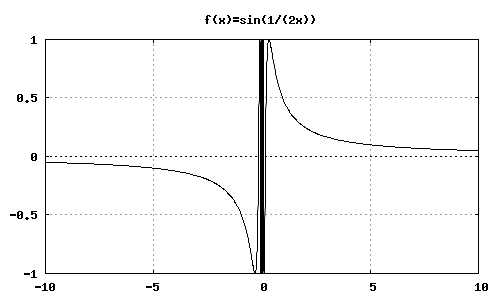
\includegraphics[width=3in]{example_3_1_2_1}

We see the horizontal asymptote at the $x$-axis, indicating that $\lim_{x \to \infty}\sin{\frac{1}{2x}}=0$.  We also see that there is a lot of activity jammed up near the $y$-axis, so we produce a second plot to highlight this interesting behavior.

\begin{verbatim}
(%i10) wxdraw2d(
       xaxis=true,
       yaxis=true,
       grid=true,
       xrange=[0,.1],
       yrange=[-1,1],
       title="f(x)=sin(1/(2x))",
       color=black,
       explicit((F(x)),x,-10,10)
       ); 
\end{verbatim}

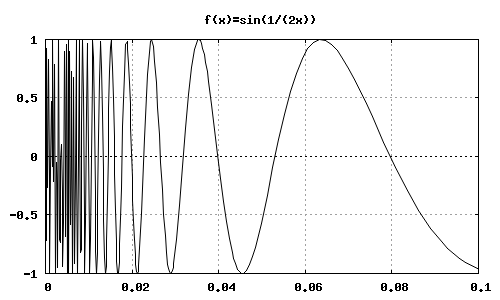
\includegraphics[width=3in]{example_3_1_2_2}

We see that $f(x)$ just keeps oscillating faster as $x$ gets closer to zero.  $\lim_{x \to 0}f(x)$ doesn't exist because $f(x)$ never gets closer to a single value as $x$ gets closer to $0$.

\end{exmp}

\line(1,0){60}
\linethickness{0.5mm}

\pagebreak

\section{wxMaxima's Limit Commands}\label{wxMaxima's Limit Commands}

The \verb|limit| command is used to compute left, right and ordinary limits in wxMaxima (the ordinary limit exists if the right and left limits both have the same value).

\begin{exmp}  

Define the function $f(x)=\frac{3x-5}{\sqrt{x^2}}$.  Compute the limits at $\pm \infty$, and compute the left and right limits at the vertical asymptote.  Use your results to make a plot of $f(x)$ together with all asymptotes plotted in red.\\
${}$\\

We see that the denominator vanishes (but the numerator does not) at $x=0$, so that should be the location of the vertical asymptote.  Note that \verb|inf| means $\infty$, \verb|minf| means $-\infty$, \verb|minus| indicates a limit from the left, and \verb|plus| indicates a limit from the right.

\begin{verbatim}
(%i1) f(x):=(3*x-5)/sqrt(x^2)$
(%i2) limit(f(x),x,minf);
(%o2) -3
(%i3) limit(f(x),x,inf);
(%o3) 3
(%i4) limit(f(x),x,0,minus);
(%o4) -inf
(%i5) limit(f(x),x,0,plus);
(%o5) -inf
\end{verbatim}

The limits at $\pm \infty$ indicate that $f(x)$ has two horizontal asymptotes, $y=-3$ and $y=+3$.  The left and right limits at $x=0$ are both $-\infty$, so there is a vertical asymptote there.  The two one-sided limits agree at $x=0$, so we can conclude the ordinary limit exists and should evaluate to $-\infty$ as well:

\begin{verbatim}
(%i6) limit(f(x),x,0);
(%o6) -inf
\end{verbatim}

Finally, we plot $f(x)$ with all its asymptotes:

\begin{verbatim}
(%i7) wxdraw2d(
      grid=true,
      xaxis=true,
      yaxis=true,
      title="f(x)=(3x-5)/sqrt(x^2)",
      xrange=[-10,10],
      yrange=[-25,5],
      color=black,
       explicit((f(x)),x,-10,10),
      color=red,
      line_type=dots,
       explicit(3,x,-10,10),
       explicit(-3,x,-10,10),
       parametric(0,t,t,-25,5)
      );
\end{verbatim}

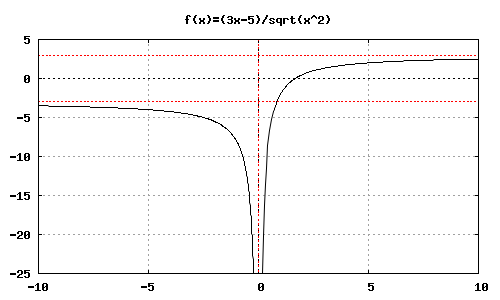
\includegraphics[width=3in]{example_3_2_1}

\end{exmp}

\line(1,0){60}
\linethickness{0.5mm}



\begin{exmp}  Compute the limits at $\pm \infty$ for the function $f(x)=e^{x}$, then plot $f(x)$ to verify that the function behaves as indicated by the limits.\\

\begin{verbatim}
(%i8) f(x):=%e^(x)$
(%i9) limit(f(x),x,minf);
(%o9) 0
(%i10) limit(f(x),x,inf);
(%o10) inf
\end{verbatim}

We obtain $\lim_{x \to -\infty}f(x)=0$ and $\lim_{x \to +\infty}f(x)=+\infty$.  Plotting $f(x)$

\begin{verbatim}
(%i11) wxdraw2d(
       grid=true,
       xaxis=true,
       yaxis=true,
       xrange=[-4,4],
       yrange=[-1,50],
       color=black,
       explicit(f(x),x,-4,4)
       );
\end{verbatim}

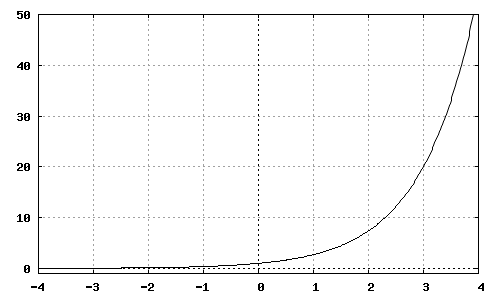
\includegraphics[width=3in]{example_3_2_2}

we see that it is asymptotic to the $x$-axis for large negative values of $x$, and it runs off to infinity for large values of $x$.

\end{exmp}

\line(1,0){60}
\linethickness{0.5mm}



\begin{exmp}  Define $f(x)=\frac{2x^2-3x+1}{x+5}$.  Find the left and right limits at the vertical asymptote and compute the limits at $\pm\infty$.  Plot $f(x)$ including the vertical asymptote and the \textit{slant} asymptote.\\
${}$\\

The vertical asymptote should appear at $x=-5$, since the denominator vanishes there.  

\begin{verbatim}
(%i12) f(x):=(2*x^2-3*x+1)/(x+5)$
(%i13) limit(f(x),x,minf);
(%o13) -inf
(%i14) limit(f(x),x,inf);
(%o14) inf
(%i15) limit(f(x),x,-5,minus);
(%o15) -inf
(%i16) limit(f(x),x,-5,plus);
(%o16) inf
\end{verbatim}

We make a preliminary plot to investigate the slant asymptote:

\begin{verbatim}
(%i17) wxdraw2d(
       grid=true,
       yaxis=true,
       xaxis=true,
       xrange=[-20,20],
       yrange=[-80,80],
       color=black,
       title="Preliminary Plot of f(x)",
       explicit((f(x)),x,-20,20)
       );
\end{verbatim}

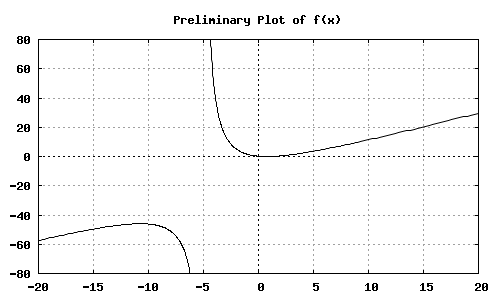
\includegraphics[width=3in]{example_3_2_3_1}


We see that $f(x)$ appears asymptotic to a tilted line as $x$ becomes large in either direction. We can get a handle on the slant asymptote by performing polynomial long division on $f(x)$ as follows:

\begin{verbatim}
(%i18) p:2*x^2-3*x+1$
       q:x+5$
(%i19) divide(p,q);
(%o19) [2*x-13,66]
\end{verbatim}


wxMaxima indicates that $f(x)=2x-13+\frac{66}{x+5}$.  As $x$ becomes large, the remainder term approaches $0$ and the slant asymptote $y=2x-13$ becomes a good fit for $f(x)$.\\
${}$\\  

Plotting $f(x)$ with all its asymptotes, we obtain:

\begin{verbatim}
(%i20) wxdraw2d(
       grid=true,
       yaxis=true,
       xaxis=true,
       xrange=[-20,20],
       yrange=[-80,80],
       title="f(x)=(2x^2-3x+1)/(x+5)",
       color=black,
        explicit((f(x)),x,-20,20),
       color=red,
       line_type=dots,
        explicit((2*x-13),x,-20,20),
        parametric(-5,t,t,-80,80)
       );
\end{verbatim}

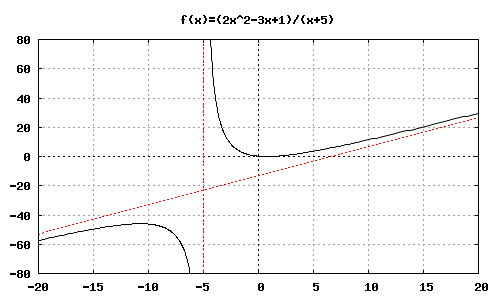
\includegraphics[width=3in]{example_3_2_3_2}

\end{exmp}

\line(1,0){60}
\linethickness{0.5mm}



\begin{exmp} Define $f(x)=\frac{1-\cos{x}}{x}$.  Compute $\lim_{x \to 0^+}f(x)$ and make a plot to verify your answer.\\
${}$\\

This is an interesting limit, because the numerator and denominator are both approaching zero:

\begin{verbatim}
(%i21) limit(1-cos(x),x,0,plus);
(%o21) 0
(%i22) limit(x,x,0,plus);
(%o22) 0
\end{verbatim}

Because $0/0$ is an indeterminate form, the ``by-hand'' calculation would require some algebraic manipulation.  wxMaxima handles it quickly:

\begin{verbatim}
(%i23) limit((1-cos(x))/x,x,0,plus);
(%o23) 0
\end{verbatim}

We verify with a quick plot:

\begin{verbatim}
(%i24) wxdraw2d(
       xaxis=true,
       yaxis=true,
       color=black,
       xrange=[-1,1],
       yrange=[-1,1],
       explicit((1-cos(x))/x,x,-1,1)
       );
\end{verbatim}

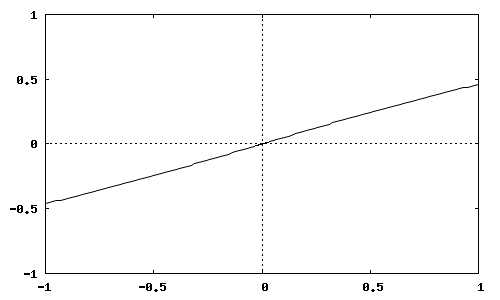
\includegraphics[width=3in]{example_3_2_4}

The plot makes it clear that $f(x) \to 0$ as $x \to 0$ (from the left as well as the right).

\end{exmp}

\line(1,0){60}
\linethickness{0.5mm}

\pagebreak


\section{Exploring the Formal Definition of Limit}\label{Exploring the Formal Definition of Limit}


The \textbf{ordinary limit} of a function $f(x)$ at $x=a$ is defined precisely as follows:\\
${}$\\
$\lim_{x \to a}f(x)=L$ if and only if, for any $\epsilon>0$ there exists a $\delta>0$ such that $|f(x)-L|<\epsilon$ when $|x-a|<\delta$.\\
${}$\\
That is, no matter how small our vertical tolerance, $\epsilon$ about $L$, we can always find a small enough $\delta$ so $f(x)$ is within $\epsilon$ of $L$ when $x$ is within $\delta$ of $a$.  This agrees with the informal definition that ``making $x$ really close to $a$ guarantees that $f(x)$ is really close to $L$''.\\
${}$  \\

A \textbf{limit at infinity} has a similar definition:\\
${}$\\
$\lim_{x \to \infty}f(x)=L$ if and only if, for any $\epsilon>0$ there exists an $N>0$ such that $|f(x)-L|<\epsilon$ when $x>N$.\\
${}$\\
That is, no matter how small our vertical tolerance, $\epsilon$ about $L$, we can always find a large enough $N$ so $f(x)$ is within $\epsilon$ of $L$ when $x$ is greater than $N$.  This agrees with the informal definition that ``making $x$ really large guarantees that $f(x)$ is really close to $L$''.\\
${}$  \\
  
Finally, an \textbf{infinite limit} can be precisely defined as follows:\\
${}$\\
$\lim_{x \to a}f(x)=\infty$ if and only if, for any $M>0$ there exists a $\delta>0$ such that $f(x)>M$ when $|x-a|<\delta$.\\
${}$\\
That is, no matter how large a $y$ value $M$ we choose, we can always find a small enough $\delta$ so that $f(x)$ exceeds $M$ when $x$ is within $\delta$ of $a$.  This agrees with the informal definition that ``making $x$ really close to $a$ makes $f(x)$ very really large''.\\
${}$  \\
  ${}$\\
The precise definition of limit is very useful for proving theorems in formal analysis.  Here, we will simply use wxMaxima to improve our \textit{intuition} about the so-called ``$\epsilon-\delta$ definition''.




\begin{exmp}  Define $f(x)=\ln(x)$.  Use wxMaxima to verify that $\lim_{x \to 2}f(x)=\ln{2}$.  Applying the formal definition of the limit, choose $\epsilon=0.1$ as the vertical tolerance about $\ln{2}$.  For this value of $\epsilon$, find a decimal approximation for $\delta$ such that $|f(x)-\ln{2}|<\epsilon$ when $|x-2|<\delta$.\\
${}$\\

Recall that wxMaxima's symbol for the natural logarithm is \verb|log|:

\begin{verbatim}
(%i1) f(x):=log(x);
(%o1) f(x):=log(x)
(%i2) limit(f(x),x,2);
(%o2) log(2)
\end{verbatim}

We have verified that $\lim_{x \to 2}f(x)=\ln{2}$, so the formal definition of this limit must be satisfied.  For $\epsilon=0.1$, we can investigate further by making a plot of $f(x)$ and using horizontal lines to map out the window of width $\epsilon$ about $\ln(2)$.  The upper $y$ value is $\ln(2)+.1$ and the lower value is $\ln(2)-.1$.

\begin{verbatim}
(%i3) wxdraw2d(
      grid=true,
      xaxis=true,
      yaxis=true,
      title="f(x)=ln(x) with interval of width epsilon about ln(2)",
      color=black,
       explicit((f(x)),x,0,3),
      color=red,
       explicit((log(2)+.1),x,0,3),
       explicit((log(2)-.1),x,0,3)
       );
\end{verbatim}

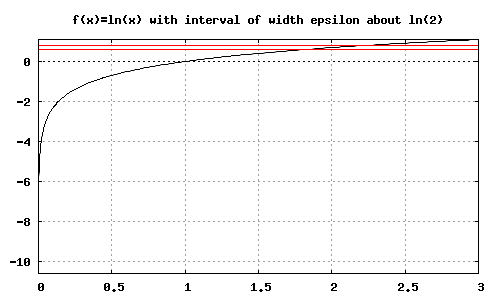
\includegraphics[width=3in]{example_3_3_1_1}



Now we should be able to find a $\delta$ sufficiently small to constrain the values of $f(x)$ within this narrow vertical range when $x$ is within $\delta$ of $2$.  In order to get the precise information, we find the intersections between $f(x)$ and the horizontal lines:

\begin{verbatim}
(%i4) float(solve(f(x)=log(2)+.1,x));
      rat: replaced -0.1 by -1/10 = -0.1
(%o4) [x=2.210341836151295]
(%i5) float(solve(f(x)=log(2)-.1,x));
      rat: replaced 0.1 by 1/10 = 0.1
(%o5) [x=1.809674836071919]
\end{verbatim}

To three decimal places, we can say that when $x$ lies on $[1.810,2.210]$, $f(x)$ is constrained to $[\ln(2)-.1,\ln(2)+.1]$.  We still need to find the $\delta$ that works in the formal definition, so we choose the \textit{smaller} of the two distances bewteen $x=2$ and the endpoints of the interval $[1.810,2.210]$; i.e., $\delta=0.19$.  Now we can say that $f(x)$ is within $0.1$ of $\ln(2)$ when $x$ is within $.19$ of $2$, and the formal definition is satisfied for $\epsilon=0.1$.\\
${}$\\
Finally, we should re-do the plot with the lines $x=2-\delta=1.81$ and $x=2+\delta=2.19$ added to illustrate how the formal definition is satisfied:

\begin{verbatim}
(%i6) wxdraw2d(
      grid=true,
      xaxis=true,
      yaxis=true,
      xrange=[1.6,2.4],
      yrange=[.4,.9],
      title="epsilon interval about y=ln(2) and delta interval about x=2",
      color=black,
       explicit((f(x)),x,0,3),
      color=red,
       explicit((log(2)+.1),x,0,3),
       explicit((log(2)-.1),x,0,3),
      color=blue,
       parametric(1.81,t,t,.4,.9),
       parametric(2.19,t,t,.4,.9)
       );
\end{verbatim}

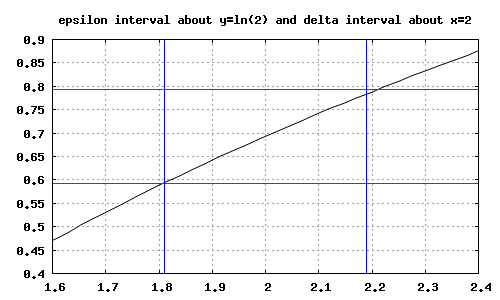
\includegraphics[width=3in]{example_3_3_1_2}

Whenever $x$ is within $[2-.19,2+.19]$ we see that $f(x)$ is within $[\ln2-.1,\ln2+.1]$.  Of course, if we chose an even smaller $\epsilon$, we could easily find a smaller $\delta$ to constrain the $y$ values to within $\epsilon$ of $\ln(2)$.


\end{exmp}

\line(1,0){60}
\linethickness{0.5mm}




\begin{exmp}  Define $f(x)=4e^{-0.3\cdot x}\cdot\sin{(3 \pi x)}+2$.  Use wxMaxima to compute the limit at positive infinity.  Once the limit is determined, illustrate the formal approach to the limit by using $\epsilon=.05$.\\
${}$\\

First, we compute the limit:

\begin{verbatim}
(%i7) f(x):=4*%e^(-.3*x)*sin(3*%pi*x)+2$
(%i8) limit(f(x),x,inf);
       rat: replaced -0.3 by -3/10 = -0.3
(%o8) 2
\end{verbatim}

We see that $\lim_{x \to \infty}f(x)=2$.  Next, we plot $f(x)$ together with the narrow window represeting our vertical tolerance of $\epsilon=0.05$ about $y=2$:

\begin{verbatim}
(%i9) wxdraw2d(
       grid=true,
       xaxis=true,
       yaxis=true,
       title="f(x) together with y=1.95 and y=2.05",
       color=black,
        explicit((f(x)),x,0,20),
       color=red,
        explicit(1.95,x,0,20),
        explicit(2.05,x,0,20)
       );
\end{verbatim}

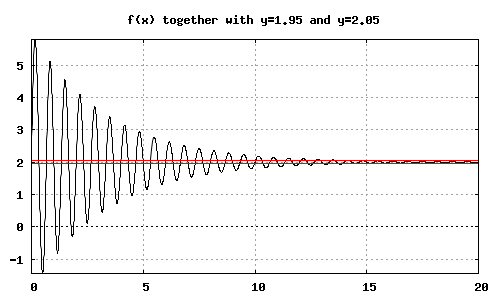
\includegraphics[width=3in]{example_3_3_2_1}

Recalling the formal definition of a limit at infinity, we search for a large enough $N$ to guarantee that $f(x)$ is within $.05$ of $2$ whenever $x>N$.  It is interesting to find the \textit{smallest} $N$ possible, and we can get a good approximation by visual inspection of the plot of $f(x)$.  We look for the final intersection between $f(x)$ and the horizontal lines $y=1.95$ and $y=2.05$, before $f(x)$ becomes constrained between the two lines forever.  We zoom in to get a better look at this intersection:

\begin{verbatim}
(%i10) wxdraw2d(
       grid=true,
       xaxis=true,
       yaxis=true,
       title="f(x) together with y=1.95 and y=2.05",
       color=black,
        explicit((f(x)),x,12,16),
       color=red,
        explicit(1.95,x,12,16),
        explicit(2.05,x,12,16)
       );
\end{verbatim}

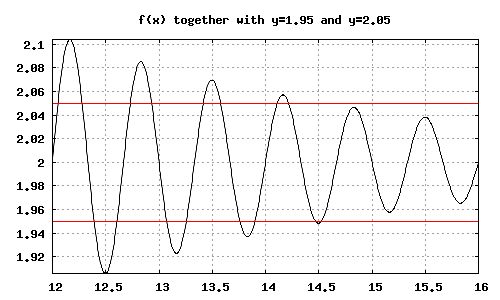
\includegraphics[width=3in]{example_3_3_2_2}

The final intersection appears to happen just to the right of $14.5$. We can nail it down to several decimal places by computing the intersection point in wxMaxima:

\begin{verbatim}
(%i11) find_root(f(x)-1.95,x,14.5,15);
(%o11) 14.52360146112245
\end{verbatim} 

To three decimal places, we conclude that when $x>14.524$, $f(x)$ is within $.05$ of $2$.  Again, we can see that a smaller $\epsilon$ would simply require us to find a larger $N$.

\end{exmp}

\line(1,0){60}
\linethickness{0.5mm}

\pagebreak

\section{Module 2 Exercises}\label{Module 2 Exercises}

\begin{enumerate}

\item  Compute $\lim_{x \to {\frac{\pi}{3}}^+} \cos{x}$ by using a ten-step do-loop with the formula $(1+\frac{1}{2^i})\frac{\pi}{3}$.

\item Compute $\lim_{x \to -3^-}\frac{2}{x+3}$ by using a 20-step do-loop (choose your own sequence).

\item  Use \verb|limit| to identify all asymptotes of $f(x)=\frac{3-5x^2}{x^2-8}$.  Make a plot of $f(x)$ including all the asymptotes in red.

\item  Use \verb|limit| to compute $\lim_{x \to 3}\frac{\sqrt{x}-\sqrt{3}}{x-3}$.

\item  Use \verb|limit| to compute $\lim_{n \to \infty}(1+\frac{1}{n})^n$  Comment on the result.

\item  For the function in Example 2.3.2, $f(x)=4e^{-0.3\cdot x}\cdot\sin{(3 \pi x)}+2$, we can study $\lim_{x \to \infty}f(x)$ by using the ``squeeze theorem''.  Substitute the maximum and minimum values of the sine function in order to obtain a curve that bounds $f(x)$ from above (call it \verb|UPPER(x)|) and a curve that bounds $f(x)$ from below  (call it \verb|LOWER(x)|).  Plot $f(x)$ with these two curves shown in red.  Finally, use \verb|limit| to show that both the upper and lower bounds approach $2$ as $x \to \infty$ (the squeeze theorem tells you that $f(x) \to 2$ as well).

\item  The \textit{derivative} of a function $f(x)$ can be written $f'(x)=\lim_{h \to 0} \frac{f(x+h)-f(x)}{h}$.  Use this definition to find the derivative of $\cos{x}$ in wxMaxima.

\item  A function $f(x)$ is \textit{continuous} at $x=a$ if $\lim_{x \to a}f(x)=f(a)$.  Use wxMaxima to show that $f(x)=\tan{x}$ is continuous at $x=\frac{\pi}{3}$.

\item The \textit{Intermediate Value Theorem} states that, for any continuous function on $[a,b]$ for which $f(a) \neq f(b)$, and any number $u$ between $f(a)$ and $f(b)$, there exists a $c$ in $(a,b)$ such that $f(c)=u$. In other words, if $f(x)$ is continuous, then all $y$ values between $f(a)$ and $f(b)$ must appear on the interval $[a,b]$. Define $f(x)=e^{-x^2}$.  Apply the Intermediate Value Theorem on the interval $[0,1]$ using $u=0.5$; i.e., find $c$.

\item Using Example 2.3.1 as a model, apply the formal definition of limit to $\lim_{x \to \frac{\pi}{2}}(\sin{x}+\cos{x})$.  Use $\epsilon = .001$.

\item Using $M=1000$, apply the formal definition of limit to illustrate that $\lim_{x \to 0}\frac{1}{x^2}=\infty$. 

\item  The \textit{unit step function} (also called the $\Theta$ function) is a piecewise defined function $\Theta(x)=\begin{cases} 0 & x<0 \\ 1 & x \geq 0 \end{cases}$.  $\Theta(x)$ is built in to wxMaxima as \verb|unit_step(x)|.  Compute $\lim_{x \to 0^-}\Theta(x)$, $\lim_{x \to 0^+}\Theta(x)$ and $\lim_{x \to 0}\Theta(x)$.  Cite a theorem to explain why the last limit does not exist.





\end{enumerate}


\pagebreak

\chapter{Introduction to Derivatives}

\vspace*{\fill}

\minitoc

\vspace*{\fill}



\flushleft{\textbf{\Large Key Commands Included in This Module}}
\newline
\newline

\begin{tabular}{l l l}
 \verb|wxdraw2d   |   &\verb|solve   |   &\verb|trigexpand   |   \\
 \verb|makelist   |   &\verb|float   |   &\verb|trigsimp   |   \\
 \verb|dimensions   |   &\verb|ev   |   &\verb|exponentialize   |   \\
 \verb|limit   |   &\verb|depends   |   &\verb|expand   |   \\
 \verb|diff   |   &\verb|subst   |   &\verb|   |   \\
\end{tabular}



\pagebreak

\section{The Tangent Line Problem}\label{The Tangent Line Problem}

\subsection{The Tangent Line from a Sequence of Secant Lines}

A \textbf{secant} is a line connecting two points on a function, $(a,f(a))$ and $(b,f(b))$.  We can approximate the slope of the \textbf{tangent} at $(a,f(a))$ by computing the slopes of secant lines on smaller and smaller intervals with $x=a$ fixed at one end.\\


\begin{exmp}  For the function $f(x)=0.5x^2-3x$, find the equation of the secant line connecting $(1,f(1))$ to $(3,f(3))$.  Make a plot of $f(x)$ together with a plot of the secant line.\\
${}$\\

Recall that the slope of a line connecting two points $(a,f(a))$ and $(b,f(b))$ is given by $m=\frac{f(b)-f(a)}{b-a}$.  We can plug this into the point-slope form to obtain $y-f(a)=\frac{f(b)-f(a)}{b-a}\cdot(x-a)$.  We solve this equation for $y$ when we define the secant line in wxMaxima.  The secant line is defined as a function of three variables, $x$, $a$ and $b$, so we can quickly find \textit{any} secant line by just changing $a$ and $b$ inside \verb|wxdraw2d|.

\begin{verbatim}
(%i1) f(x):=0.5*x^2-3*x$
(%i2) SECANT(x,a,b):=((f(b)-f(a))/(b-a))*(x-a)+f(a)$
(%i3) wxdraw2d(
      grid=true,
      xaxis=true,
      yaxis=true,
      title="f(x) with a secant line",
      color=black,
       explicit((f(x)),x,0,4),
      color=red,
       explicit((SECANT(x,1,3)),x,0,4)
      );
\end{verbatim}


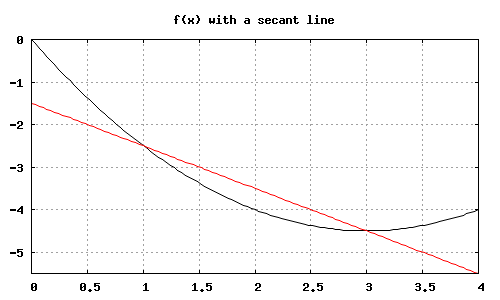
\includegraphics[width=3in]{example_4_1_1}


\end{exmp}

\line(1,0){60}
\linethickness{0.5mm}


\begin{exmp}  For $f(x)=\sqrt{9-x^2}$, use a do-loop to compute the slopes of secant lines on $[-2,0],[-2,-.1],[-2,-.2],\dots,[-2,-1.9]$.  Use \verb|makelist| to plot the secant lines in red together with $f(x)$ in black.\\
${}$\\

We use formula $0.1-0.1\cdot i$ to generate the sequence of right-hand points.  We use \verb|for-do| to compute the sequence of slopes and \verb|makelist| to compute the equations of all the secant lines.  Note that the list has to be ready to import into \verb|wxdraw2d| -- we include \verb|explicit| and the $x$ range in each list element.  Finally, we use \verb|dimensions| to make the semi-circle $f(x)$ appear properly. 

\begin{verbatim}
(%i4) f(x):=sqrt(9-x^2)$
(%i5) SLOPE(a,b):=(f(b)-f(a))/(b-a)$
(%i6) SECANT(x,a,b):=SLOPE(a,b)*(x-a)+f(a)$
(%i7) (print ("interval",".........","slope"),
       for i:1 thru 20 do
       (S:float(SLOPE(-2,0.1-0.1*i)),
        print("[-2,",0.1-0.1*i,"]",".........",S))
       );
       
 interval.........slope
[-2, 0.0].........0.38196601125011
[-2,-0.1].........0.40119204874379
[-2,-0.2].........0.42069885106631
[-2,-0.3].........0.44052607871769
[-2,-0.4].........0.46071610747744
[-2,-0.5].........0.48131460936668
[-2,-0.6].........0.50237122417145
[-2,-0.7].........0.52394034743321
[-2,-0.8].........0.54608206788367
[-2,-0.9].........0.56886329704641
[-2,-1.0].........0.5923591472464
[-2,-1.1].........0.61665463321198
[-2,-1.2].........0.64184679934214
[-2,-1.3].........0.66804741345624
[-2,-1.4].........0.69538642464088
[-2,-1.5].........0.72401646770705
[-2,-1.6].........0.75411882647529
[-2,-1.7].........0.78591147120622
[-2,-1.8].........0.81966011250105
[-2,-1.9].........0.8556937574899
(%o7) done

(%i8) L:makelist(explicit(SECANT(x,-2,.1-.1*i),x,-3,3),i,1,20)$
(%i9) wxdraw2d(
      grid=true,
      xaxis=true,
      dimensions=[600,600],
      title="f(x)=sqrt(9-x^2) with secant lines approaching a tangent",
      color=black,
       explicit(f(x),x,-3,3),
      color=red,
       L
      );
\end{verbatim}


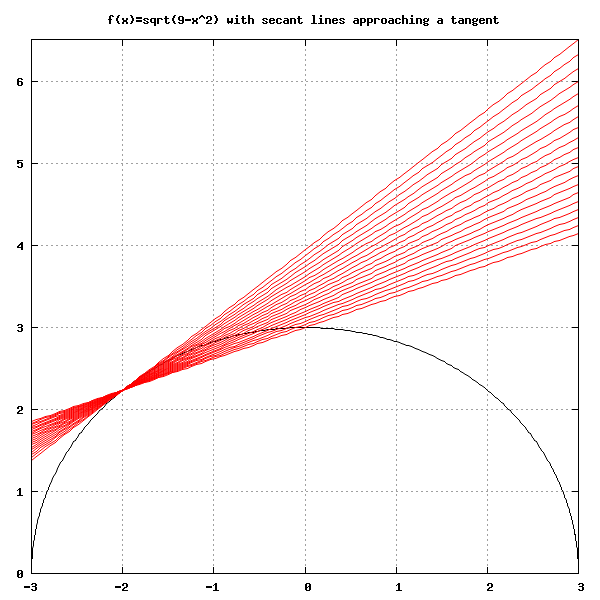
\includegraphics[width=3in]{example_4_1_2}

As the interval gets smaller and smaller (with $-2$ always the left side of the interval), the secant lines rotate counter-clockwise and become closer and closer to the tangent line at $x=-2$.  The slope of the tangent line appears to be slightly less than $1$, which agrees with the output of our do-loop.


\end{exmp}

\line(1,0){60}
\linethickness{0.5mm}

\subsection{The Tangent Line as a Limit}

The limit process in the previous Example can be generalized to find the exact slope of the tangent line to $f(x)$ at $x=a$.  We compute the slope of the secant line connecting $(a,f(a))$ and $(a+h,f(a+h))$, then we take the limit as $h \to 0$.  An alternative notation is that we take the slope of the secant line connecting $(a,f(a))$ and $(x,f(x))$, then take the limit as $x \to a$.  The slope of the tangent line at $x=a$ is called the \textbf{derivative} of $f(x)$ at $x=a$, written $f'(a)$:

\[f'(a)=\lim_{h \to 0}\frac{f(a+h)-f(a)}{h} =\lim_{x \to a}\frac{f(x)-f(a)}{x-a}\]

${}$\\

\begin{exmp}  Define $f(x)=\tan{x}$, then use the ``limit definition'' of the derivative to compute $f'(1)$.  Finally, produce a plot of $f(x)$ together with the tangent line at $(1,f(1))$.\\
${}$\\

We can use either ``limit definition'' to find $f'(1)$:

\begin{verbatim}
(%i10) f(x):=tan(x)$

(%i11) limit(((f(1+h)-f(1))/(h)),h,0);
(%o11) 1/cos(1)^2

(%i12) limit(((f(x)-f(1))/(x-1)),x,1);
(%o12) 1/cos(1)^2
\end{verbatim}

We see that $f'(1)=\frac{1}{\cos^2{1}}$.  The equation of the tangent line is then computed using the fact that the slope is $f'(1)$ at the point $(1,f(1))$ (we solve the point-slope form for $y$).

\begin{verbatim}
(%i13) SLP:%$
(%i14) TNGT(x):=SLP*(x-1)+f(1)$
(%i15) wxdraw2d(
       grid=true,
       xaxis=true,
       yaxis=true,
       xrange=[-2,2],
       yrange=[-10,10],
       title="f(x)=tan(x) with the tangent line at x=1",
       color=black,
        explicit((f(x)),x,-2,2),
       color=red,
        explicit((TNGT(x)),x,-2,2)
       );
       
\end{verbatim}

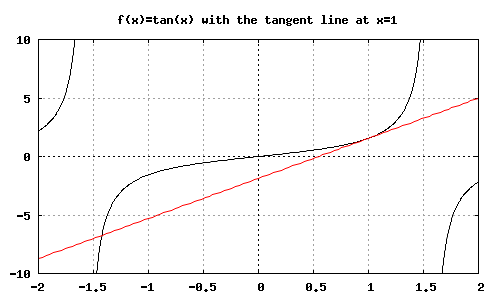
\includegraphics[width=3in]{example_4_1_3}


We see that the tangent line behaves appropriately at $x=1$.

\end{exmp}

\line(1,0){60}
\linethickness{0.5mm}



\begin{exmp} Define $f(x)=x^n$, then use the limit definition of the derivative to find a general formula for $f'(x)$ (this formula is sometimes called the ``power rule'').\\
${}$\\

This is just one example of how the formulas are derived for the ``algebra of derivatives'':  every rule comes from the computation of a limit.  We evaluate the derivative at $x=X$ to emphasize that the result is valid for \textit{any} real number.

\begin{verbatim}
(%i16) f(x):=x^n$
(%i17) limit(((f(x)-f(X))/(x-X)),x,X);
(%o18) n*X^(n-1)
\end{verbatim}

We conclude that, if $f(x)=x^n$, then $f'(x)=n\cdot x^{n-1}$ for any value of $x$.  We can view $f'(x)$ as a new \textit{function} of $x$ that tells us the slope of $f(x)$ at any value of $x$.

\end{exmp}

\line(1,0){60}
\linethickness{0.5mm}

\pagebreak

\section{wxMaxima's Derivative Commands}\label{wxMaxima's Derivative Commands}

As you might expect, wxMaxima can quickly find the derivative of a function using the \verb|diff| command:

\begin{exmp}  For the function $f(x)=\tan^{-1}{x}$: \\
${}$   \\
\verb|         |a. compute $f'(1.5)$
\verb|         |b. find all $x$ such that $f'(x)=\frac{1}{2}$\\
${}$\\

a.  Note that we have to use \verb|''| when defining a new function as the derivative of an old function.  This makes wxMaxima compute the general expression for $f'(x)$ \textit{before} it attempts to substitute particular values of $x$ (substituting $x=1.5$ into \verb|diff(f(x),x)| produces an error).

\begin{verbatim}
(%i1) f(x):=atan(x)$
(%i2) f_prime(x):=''(diff(f(x),x));
(%o2) f_prime(x):=1/(x^2+1)
(%i3) f_prime(1.5);
(%o3) 0.30769230769231
\end{verbatim}

b.  We use \verb|solve| to find the $x$ values for which $f'(x)=0.5$:

\begin{verbatim}
(%i4) solve(f_prime(x)=0.5,x);
rat: replaced -0.5 by -1/2 = -0.5
(%o4) [x=-1,x=1]
\end{verbatim} 

It is worth checking this answer graphically.  We will plot $f(x)$ together with the tangent lines at $x=\pm 1$::

\begin{verbatim}
(%i5) TANGENT(x,a):=f_prime(a)*(x-a)+f(a)$
(%i6) wxdraw2d(
      grid=true,
      xaxis=true,
      yaxis=true,
      title="The arctangent function with two tangent lines at x=+/- 1",
      color=black,
       explicit((f(x)),x,-3,3),
      color=red,
       explicit((TANGENT(x,-1)),x,-3,3),
       explicit((TANGENT(x,1)),x,-3,3)
      );
\end{verbatim}


\includegraphics[width=3in]{example_4_2_1}

We see that these two tangent lines are the only tangent lines with slope $\frac{1}{2}$.


\end{exmp}

\line(1,0){60}
\linethickness{0.5mm}



\begin{exmp} Define $f(x)=2\sin{x}$.  Use wxMaxima to compute $f'(x)$.  Compute the equation of the tangent line to $f(x)$ at $x=2$.  Finally, plot $f(x)$, $f'(x)$ and the tangent line at $x=2$.  Comment on the slope relationship between $f(x)$ and $f'(x)$ at $x=2$.\\

\begin{verbatim}
(%i7) f(x):=2*sin(x)$
(%i8) f_prime(x):=''(diff(f(x),x))$
(%i9) TANGENT(x,a):=f_prime(a)*(x-a)+f(a)$
(%i10) wxdraw2d(
       grid=true,
       xrange=[-5,5],
       yrange=[-5,5],
       dimensions=[600,600],
       title="f(x)=2sin(x), f_prime(x), and a tangent line at x=2",
       color=black,
        explicit((f(x)),x,-5,5),
       color=grey,
        explicit((f_prime(x)),x,-5,5),
       color=red,
        explicit((TANGENT(x,2)),x,-5,5)
       );
\end{verbatim}

\includegraphics[width=3in]{example_4_2_2}

The slope of the tangent line to $f(x)$ is slightly greater than $-1$ (we set \verb|dimensions| in the plot to make it easier to estimate).  Correspondingly, the graph of $f'(x)$ has a $y$ coordinate slightly greater than $-1$ at $x=2$.  A decimal approximation is found quickly in wxMaxima:

\begin{verbatim}
(%i11) float(f_prime(2));
(%o11) -0.83229367309428
\end{verbatim}

It is important to be able to ``eyeball'' the graph of a function and sketch its derivative in this way -- the derivative function has $y$ values equal to the \textit{slope} of $f(x)$ at each value of $x$.

\end{exmp}

\line(1,0){60}
\linethickness{0.5mm}

\begin{exmp}

Define $f(x)=\sin^5{(x)} \cdot e^x-\cos^2{x}$ and find its first three derivatives.  Use \verb|trigsimp| to simplify according to pythagorean identities.\\
${}$\\

The point of this example is simply to illustrate how wxMaxima handles higher order derivatives that would be very tedious if done by hand!\\

\verb|(%i12) f(x):=(sin(x))^5*%e^x-(cos(x))^2;|\\
\verb|(%o12) | $\mathrm{f}\left( x\right) :={\mathrm{sin}\left( x\right) }^{5}\,{e}^{x}-{\mathrm{cos}\left( x\right) }^{2}$\\
\verb|(%i13) diff(f(x),x);|\\
\verb|(%o13) | ${e}^{x}\,{\mathrm{sin}\left( x\right) }^{5}+5\,{e}^{x}\,\mathrm{cos}\left( x\right) \,{\mathrm{sin}\left( x\right) }^{4}+2\,\mathrm{cos}\left( x\right) \,\mathrm{sin}\left( x\right) $\\
\verb|(%i14) diff(f(x),x,2);|\\
\verb|(%o14) | $-4\,{e}^{x}\,{\mathrm{sin}\left( x\right) }^{5}+10\,{e}^{x}\,\mathrm{cos}\left( x\right) \,{\mathrm{sin}\left( x\right) }^{4}+20\,{e}^{x}\,{\mathrm{cos}\left( x\right) }^{2}\,{\mathrm{sin}\left( x\right) }^{3}-2\,{\mathrm{sin}\left( x\right) }^{2}$\\
\verb|       |$+2\,{\mathrm{cos}\left( x\right) }^{2}$\\
\verb|(%i15) trigsimp(%);|\\
\verb|(%o15) | $-24\,{e}^{x}\,{\mathrm{sin}\left( x\right) }^{5}+10\,{e}^{x}\,\mathrm{cos}\left( x\right) \,{\mathrm{sin}\left( x\right) }^{4}+20\,{e}^{x}\,{\mathrm{sin}\left( x\right) }^{3}-4\,{\mathrm{sin}\left( x\right) }^{2}+2$\\
\verb|(%i16) diff(f(x),x,3);|\\
\verb|(%o16) | $-14\,{e}^{x}\,{\mathrm{sin}\left( x\right) }^{5}-50\,{e}^{x}\,\mathrm{cos}\left( x\right) \,{\mathrm{sin}\left( x\right) }^{4}+60\,{e}^{x}\,{\mathrm{cos}\left( x\right) }^{2}\,{\mathrm{sin}\left( x\right) }^{3}+60\,{e}^{x}\,{\mathrm{cos}\left( x\right) }^{3}\,{\mathrm{sin}\left( x\right) }^{2}-8\,\mathrm{cos}\left( x\right) \,\mathrm{sin}\left( x\right) $\\
\verb|(%i17) trigsimp(%);|\\
\verb|(%o17) | $-74\,{e}^{x}\,{\mathrm{sin}\left( x\right) }^{5}-110\,{e}^{x}\,\mathrm{cos}\left( x\right) \,{\mathrm{sin}\left( x\right) }^{4}+60\,{e}^{x}\,{\mathrm{sin}\left( x\right) }^{3}+60\,{e}^{x}\,\mathrm{cos}\left( x\right) \,{\mathrm{sin}\left( x\right) }^{2}-8\,\mathrm{cos}\left( x\right) \,\mathrm{sin}\left( x\right) $

\end{exmp}

\line(1,0){60}
\linethickness{0.5mm}
\pagebreak

\section{Products, Quotients and Linear Combinations}\label{Products, Quotients and Linear Combinations}

The derivative of a product, quotient or linear combination of functions can be broken down into the derivatives of the component functions:\\


\begin{align*}
&\text{The Product Rule:} & &\frac{\mathrm{d}}{\mathrm{d}x}[f(x)\cdot g(x)]=f'(x)\cdot g(x)+f(x)\cdot g'(x)\\ \\
&\text{The Quotient Rule:} & &\frac{\mathrm{d}}{\mathrm{d}x}\frac{f(x)}{g(x)}=\frac{f'(x)\cdot g(x)-f(x)\cdot g'(x)}{[g(x)]^2}\\ \\
&\text{Linear Combinations:} & &\frac{\mathrm{d}}{\mathrm{d}x}[a\cdot f(x)+b\cdot g(x)]=a\cdot f'(x)+b\cdot g'(x)
\end{align*}

${}$\\

\begin{exmp}

Verify the quotient rule for the functions $f(x)=\sin{x}$ and $g(x)=\cos{x}$.\\

\begin{verbatim}
(%i1) f(x):=sin(x)$
      g(x):=cos(x)$
      f_prime(x):=(diff(f(x),x))$
      g_prime(x):=(diff(g(x),x))$
(%i2) (f_prime(x)*g(x)-f(x)*g_prime(x))/(g(x))^2;
(%o2) (sin(x)^2+cos(x)^2)/cos(x)^2
(%i3) trigsimp(%);
(%o3) 1/cos(x)^2
\end{verbatim}

We recognize that $\frac{\sin{x}}{\cos{x}}=\tan{x}$ and that $\frac{\mathrm{d}}{\mathrm{d}x}\tan{x}=\sec^2{x}$ as expected.  Note that \verb|trigsimp| was required to force wxMaxima to apply pythagorean identities to the result.  Verifying directly, we obtain:

\begin{verbatim}
(%i4) diff((sin(x)/cos(x)),x);
(%o4) sin(x)^2/cos(x)^2+1
(%i5) trigsimp(%);
(%o5) 1/cos(x)^2
\end{verbatim}

\end{exmp}

\line(1,0){60}
\linethickness{0.5mm}


\begin{exmp}

The basic hyperbolic functions are defined as: $\cosh{x}=\frac{1}{2}(e^x+e^{-x})$ and $\sinh{x}=\frac{1}{2}(e^x-e^{-x})$.  Use the linear combination rule to find the derivatives of these two functions, then use the quotient rule to find the derivative of $\tanh{x}=\frac{\sinh{x}}{\cosh{x}}$.\\
${}$\\

We manually use the linear combination rule and the quotient rule, but we use wxMaxima for everything else:

\begin{verbatim}
(%i6) POS:%e^x$
      NEG:%e^(-x)$
(%i7) POS_prime:diff(POS(x),x)$
      NEG_prime:diff(NEG(x),x)$
(%i8) COSH:0.5*POS+0.5*NEG$
      SINH:0.5*POS-0.5*NEG$      
(%i9) COSH_prime:0.5*POS_prime+0.5*NEG_prime;
      SINH_prime:0.5*POS_prime-0.5*NEG_prime;
(%o9) 0.5*%e^x-0.5*%e^(-x)
(%o10) 0.5*%e^x+0.5*%e^(-x)
\end{verbatim}

We see that $(\cosh{x})'=\sinh{x}$ and $(\sinh{x})'=\cosh{x}$.  The hyperbolic functions are built into wxMaxima, so we can check our work by differentiating directly:

\begin{verbatim}
(%i10) diff(cosh(x),x);
(%o10) sinh(x)
(%i11) diff(sinh(x),x);
(%o11) cosh(x)
\end{verbatim}

Applying the quotient rule ``manually'' to find $(\tanh{x})'$, we obtain:

\begin{verbatim}
(%i12) TANH_prime:(SINH_prime*COSH -SINH*COSH_prime)/(COSH^2);
(%o12) ((0.5*%e^x+0.5*%e^(-x))^2-(0.5*%e^x-0.5*%e^(-x))^2)
       /(0.5*%e^x+0.5*%e^(-x))^2
(%i13) expand(%);
(%o13) 1.0/(0.25*%e^(2*x)+0.25*%e^(-2*x)+0.5)
\end{verbatim}

We check our work by differentiating the hyperbolic tangent directly and applying \verb|exponentialize| to convert to exponential functions:

\begin{verbatim}
(%i14) diff(tanh(x),x);
(%o14) sech(x)^2
(%i15) exponentialize(%);
(%o15) 4/(%e^x+%e^(-x))^2
(%i16) expand(%);
(%o16) 4/(%e^(2*x)+%e^(-2*x)+2)
\end{verbatim}

We can divide this by 4 in in the numerator and denominator to obtain the original expression.
\end{exmp}

\line(1,0){60}
\linethickness{0.5mm}
\pagebreak





\section{Derivatives of Function Compositions}\label{Derivatives of Function Compositions}

\subsection{The Chain Rule}

The \textbf{chain rule} is a rule for differentiating function compositions.  For example, if $h(x)=g(f(x))$, then $h'(x)=g'(f(x))f'(x)$; that is, we compute $g'(x)$ but evaluate it at $f(x)$, then tack on a factor of $f'(x)$.  In the physical sciences, it is typical to use Leibniz notation as a mnemonic:  $\frac{\mathrm{d} h}{\mathrm{d} x} = \frac{\mathrm{d} h}{\mathrm{d}f} \cdot \frac{\mathrm{d}f}{\mathrm{d}x}$, which means we differentiate the entire function $h(x)$ with respect to $f(x)$ (treating $f(x)$ as a single variable), then we tack on a factor of $f'(x)$.


\begin{exmp}Two ways to look at the chain rule.\\
${}$   \\
 a.  To illustrate the chain rule in Newton's notation, find the derivative of $h(x)=e^{x^2}$ by defining $f(x)$ and $g(x)$ such that $h(x)=g(f(x))$ and computing $g'(f(x))\cdot f'(x)$. \\

\begin{verbatim}
(%i1) f(x):=x^2$
       g(x):=%e^x$
       h(x):=g(f(x))$
(%i2) ev(h(x));
(%o2) %e^x^2
(%i3) g_prime(x):=''(diff(g(x),x));
(%o3) g_prime(x):=%e^x
(%i4) g_prime(f(x))*diff(f(x),x);
(%o4) 2*x*%e^x^2
\end{verbatim}


   
b.  To illustrate the chain rule using the ``Leibniz mnemonic'', first define the function $h(x)=e^{x^2}$ as $e^{f}$, where $f$ is understood to be $x^2$.  Multiply $\frac{\mathrm{d}h}{\mathrm{d}f}$ and $\frac{\mathrm{d}f}{\mathrm{d}x}$ to construct the derivative of $h$.\\


\begin{verbatim}
(%i5) h:%e^f$
      dh_df:diff(h,f);
(%o5) %e^f
(%i6) f:x^2$
      df_dx:diff(f,x);
(%o6) 2*x
(%i7) dh_df*df_dx;
(%o7) 2*%e^f*x
(%i8) ev(%);
(%o8) 2*x*%e^x^2
\end{verbatim}

We obtain the same result.  Note that \verb|ev%| had to be used to get wxMaxima to simplify the final result.


\end{exmp}

\line(1,0){60}
\linethickness{0.5mm}

${}$\\

The chain rule can be extended naturally to compositions of more than two functions.  If $i(x)=h(g(f(x)))$ then we apply the chain rule twice: $i'(x)=h'(g(f(x)))\cdot(g(f(x)))'= h'(g(f(x)))g'(f(x))f'(x)$.  The equivalent mnemonic in Leibniz notation is $\frac{\mathrm{d} i}{\mathrm{d} x} = \frac{\mathrm{d} i}{\mathrm{d}g} \cdot \frac{\mathrm{d}g}{\mathrm{d}f} \cdot \frac{\mathrm{d}f}{\mathrm{d}x} $.  The mnemonic is much more elegant than the prime notation (which has grown quite ugly):  it tells us to differentiate $i$ with respect to $g$ (treating $g$ as a single variable), then differentiate $g$ with respect to $f$ (treating $f$ as a single variable), then differentiate $f$ with respect to $x$. 

\begin{exmp}  Let $i(x)=\sqrt{\sin^2{x}+2}$.  Find $i'(x)$ by performing the three derivatives $\frac{\mathrm{d} i}{\mathrm{d}g}, \frac{\mathrm{d}g}{\mathrm{d}f}, \text{ and } \frac{\mathrm{d}f}{\mathrm{d}x}$.  Check your answer by directly computing $i'(x)$.\\

\begin{verbatim}
(%i9) i:sqrt(g)$
      di_dg:(diff(i,g));
(%o9) 1/(2*sqrt(g))
(%i10) g:f^2+2$
      dg_df:(diff(g,f));
(%o10) 2*f
(%i11) f:sin(x)$
      df_dx:(diff(f,x));
(%o11) cos(x)
(%i12) di_dg*dg_df*df_dx;
(%o12) (f*cos(x))/sqrt(g)
(%i13) ev(%);
(%o13) (cos(x)*sin(x))/sqrt(f^2+2)
(%i14) ev(%);
(%o14) (cos(x)*sin(x))/sqrt(sin(x)^2+2)
\end{verbatim}

Note that the \verb|ev%| command had to be used twice to encourage wxMaxima to make the proper substitutions.  Checking our answer:

\begin{verbatim}
(%i15) diff(sqrt((sin(x))^2+2),x);
(%o15) (cos(x)*sin(x))/sqrt(sin(x)^2+2)
\end{verbatim}
\end{exmp}

\line(1,0){60}
\linethickness{0.5mm}

\subsection{Logarithmic Differentiation}

Recall the differentiation formula $(\ln{x})'=\frac{1}{x}$.  Now suppose that $y$ depends $x$, and we wish to differentiate a function $g(x)=\ln{y}$.  The chain rule tells us that $g'(x)=\frac{1}{y}\cdot y'(x)$.  This can provide a useful trick for finding $y'(x)$ when troublesome exponents appear in the expression for $y(x)$.  The technique is known as \textbf{logarithmic differentiation}.

\begin{exmp}  Compute the first derivative of $x^x$ by using logarithmic differentiation step-by-step.  Verify your answer by directly computing the derivative.\\

\begin{verbatim}
(%i16) EQN1:y=x^x;
(%o16) y=x^x
(%i17) EQN2:log(EQN1);
(%o17) log(y)=x*log(x)
(%i18) depends(y,x)$
(%i19) EQN3:diff(EQN2,x);
(%o19) (dy/dx)/y=log(x)+1
(%i20) EQN4:y*EQN3;
(%o20) (dy/dx)=(log(x)+1)*y
(%i21) subst(x^x,y,EQN4);
(%o21) (d/dx)x^x=x^x*(log(x)+1)
\end{verbatim}

We see that $\frac{\mathrm{d}}{\mathrm{d}x} x^x = x^x\cdot (\ln{x}+1)$.  Checking our answer:


\begin{verbatim}
(%i22) y:x^x$
       diff(y,x);
(%o22) x^x*(log(x)+1)
\end{verbatim}

\end{exmp}

\line(1,0){60}
\linethickness{0.5mm}

\subsection{Implicit Differentiation}

When a formula can only be defined implicitly (that is, we cannot solve for $y$ as a function of $x$), we can take advantage of the chain rule to compute $y'(x)$ as a function of both $x$ and $y$.  To perform \textbf{implicit differentiation}, we simply differentiate both sides of the formula with respect to $x$, then solve for $y'(x)$.  We just have to keep in mind that $\frac{\mathrm{d}}{\mathrm{d}x}f(y)=\frac{\mathrm{d}f}{\mathrm{d}y}\cdot\frac{\mathrm{d}y}{\mathrm{d}x}$.

\begin{exmp}  Use implicit differentiation to find the slope of a tangent line to the unit circle at any point (as a function of $x$ and $y$).  Use your answer to plot the tangent line at the point $(-\frac{1}{2},-\frac{\sqrt{3}}{2})$.\\
${}$\\

The unit circle has the formula $x^2+y^2=1$, which cannot be explicitly solved for $y$ without breaking it into two functions.  We find $y'(x)$ by simply differentiating the formula on both sides and algebraically isolating $\frac{\mathrm{d}y}{\mathrm{d}x}$:



\begin{verbatim}
(%i23) kill(all)$
(%i1) UNITCIRC:x^2+y^2=1$
(%i2) depends(y,x)$
(%i3) EQN1:diff(UNITCIRC,x);
(%o3) 2*y*(dy/dx)+2*x=0
(%i4) EQN2:EQN1-2*x;
(%o4) 2*y*(dy/dx)=-2*x
(%i5) EQN3:EQN2/(2*y);
(%o5) (dy/dx)=-x/y
\end{verbatim}

We see that $\frac{\mathrm{d}y}{\mathrm{d}x}=-\frac{x}{y}$.  Now we substitute the point $(-\frac{1}{2},-\frac{\sqrt{3}}{2})$, compute a tangent line and plot along with the unit circle.

\begin{verbatim}
(%i6) kill(all)$
(%i1) SLOPE:-(-1/2)/(-sqrt(3)/2)$
(%i2) TANGENT(x):=SLOPE*(x+1/2)-sqrt(3)/2$
(%i3)  wxdraw2d(
       grid=true,
       dimensions=[600,600],
       xaxis=true,
       yaxis=true,
       xrange=[-2,2],
       yrange=[-2,2],
       title="The unit circle with a tangent line",
       color=black,
        implicit((x^2+y^2=1),x,-1,1,y,-1,1),
       color=red,
        explicit((TANGENT(x)),x,-2,2)
       );
\end{verbatim}

\includegraphics[width=3in]{example_4_3_4}



\end{exmp}

\line(1,0){60}
\linethickness{0.5mm}

\pagebreak


\section{Module 3 Exercises}\label{Module 3 Exercises}

\begin{enumerate}

\item Define the function $f(x)=(x-2)(x)(x+1)$.  In the style of Example 3.1.2, find the slope of the tangent line at $x=1$ by using \verb|makelist| to generate a sequence of ten intervals $[1,2],[1,1.5],[1,1.25]...$.  Make a plot of $f(x)$ together with the sequence of secant lines approaching the tangent line.
\item Use the ``limit definition'' of the derivative to compute derivative formulas for the following functions, then verify using \verb|diff|.\\
\verb|   |\\
\verb|     |a.  $f(x)=\tan{x}$ \verb|     |b.  $f(x)=\sec{x}$ \verb|     |c.  $f(x)=\ln{(\cos{x})}$
\item Define $f(x)=\sec{x}$.  Use \verb|diff| to find the slope of the tangent line at $x=1.2$.  Finally, plot $f(x)$ together with the tangent line.

\item Use the definitions of $\cosh{x}$ and $\sinh{x}$ and the ``product rule'' to find $\frac{\mathrm{d}}{\mathrm{d}x}(\cosh{x}\cdot \sinh{x})$ ``manually''in the style of Example 3.3.2. Verify your answer by using \verb|diff| and wxMaxima's built in \verb|cosh| and \verb|sinh| functions.  Some simplification will be necessary to verify your answer!

\item When computing the derivative of a complicated trigonometric function, it can be helpful to simplify the result using \verb|trigsimp| (simplifies using pythagorean identities), \verb|trigreduce| (simplifies using sum of angles identities), \verb|trigexpand| (expands using sum of angles identities) and/or \verb|trigrat| (simplifies rational expressions of trig functions).  Define $f(x)=\sin{x} \cdot \cos^{2}{(2x)}$ and find $f'(x)$ using \verb|diff|.  Use \verb|trigexpand| then \verb|trigsimp| to express your answer entirely in terms of powers of $\cos{x}$.

\item Following the style of Example 3.4.1 and Example 3.4.2, compute $\frac{\mathrm{d}h}{\mathrm{d}x}$ for \\
\verb|   |\\
\verb|     |a. $h(x)=\cos{(3x^3-4x+5)}$  \verb|     |b.  $h(x)=e^{\sqrt{\sin{x}}}$\\
\verb|   |\\
Remember to use \verb|kill(all)| if previous assignments are interfering with your calculations.

\item Compute the fifth derivative of $f(x)=\sec{x}$ and simplify as much as possible.

\item The Mean Value Theorem states that (provided a function is continuous on $[a,b]$ and differentiable on $(a,b)$), we can always find $x=c$ on $(a,b)$ for which the slope of the tangent line is equal to the slope of the secant line connecting $(a,f(a))$ and $(b,f(b))$.  That is, we can find $c$ such that $f'(c)=\frac{f(b)-f(a)}{b-a}$.  For the function $f(x)=\tan^{-1}{x}$, find $c$ for the interval $[0.5,2.5]$.  Plot $f(x)$ in black together with the appropriate secant and tangent lines in red.  Comment on the geometric relationship between the secant line and the tangent line.

\item Let $y=\cos^{-1}{x}$.  To derive the formula for $\frac{\mathrm{d}y}{\mathrm{d}x}$, we have to invert the formula as $\cos{y}=x$ and use implicit differentiation.  Following the style of Example 3.4.4, compute $\frac{\mathrm{d}y}{\mathrm{d}x}$, including a final step of substituting the original definition of $y$ and simplifying the result if necessary to obtain an explicit formula for $y'(x)$.

\item To perform a ``linear approximation'', we use $f(a)$ and $f'(a)$ to draw a tangent line at $x=a$.  Then (as long as $\Delta{x}$ is relatively small), we can approximate $f(a+\Delta{x})$ by using the equation of the tangent line instead of $f(x)$ itself. This is a special case of a truncated \textit{Taylor series} -- a trick that it used often in physical sciences to simplify a mathematical model.  \\
${}$\\
Define $f(x)=\sin{x}$ and find the equation of the tangent line at $x=0$.  Call your tangent line $T(x)$.  Now use your tangent line to make a linear approximation to $f(0.1)$; i.e., compute $T(0.1)$.  Compare to the \textit{actual} value of $f{(0.1})$.  How much error does the linear approximation make?  Make a plot of $f(x)$ and $T(x)$ on $[0,0.2]$ to highlight the behavior of the linear approximation near $x=0$.

\item The \textit{binomial approximation} is another useful linear approximation.  Suppose that $f(x)=(1+x)^{50}$.  Use a linear approximation near $x=0$ to estimate $1.05^{50}$.  Check your answer by \textit{actually} computing $1.05^{50}$ and computing the error committed by the approximation.  Note:  this approximation is most useful for simplifying a \textit{variable} expression $(1+x)^n$ based on the assumption that $x$ is ``small''.

\item For the ellipse $\frac{(x-2)^2}{4}+\frac{(y+3)^2}{25}=1$, use implicit differentiation to find an expression for $\frac{\mathrm{d}y}{\mathrm{d}x}$ as a function of both $x$ and $y$.  Find equations for both tangent lines that have slope $\frac{1}{2}$. In order to find the points with slope $\frac{1}{2}$ you will have to solve a \textit{system} of equations:  one for the derivative and one for the original ellipse.  The proper syntax for solving a system is \verb|solve([equation1,equation2],[x,y]);|. 

${}$\\

Find equations for both tangent lines perpendicular to those with slope $\frac{1}{2}$.  Finally, plot the ellipse in black with all four tangent lines shown in red.  Use \verb|dimensions| to force the ellipse to appear with the correct aspect ratio.

\item Find the five function generalization of the product rule.  That is, find a general expression for $\frac{\mathrm{d}}{\mathrm{d}x}[f(x)\cdot g(x)\cdot h(x)\cdot i(x) \cdot j(x)]$

\item In one dimension, the position of a particle is given by its $x$-coordinate.  A moving particle will have different $x$ values at different times, and we can plot its motion using ordered pairs $(t,x)$ to produce a plot called a \textit{position-time} graph.  Position is a \textit{function} of time, $x(t)$, since at any given time, a particle can only be in one place!  The average velocity between two moments in time is given by the simple ratio $v_{avg}=\frac{x_2-x_1}{t_2-t_1}$.  Unless otherwise stated, this book will always use meters (m) for distance units and seconds (s) for time units, so $v_{avg}$ must have units of m/s.\\
${}$\\
Suppose that a rocket is observed to have the approximate position function \\ $x(t)=2.35 \cdot x^3-5.1 \cdot x^2+4$.  

 \begin{enumerate}
 
 \item Find the average velocity from $t=2 \mathrm{s}$ to $t=3 \mathrm{s}$; i.e., find $v_{avg}$ on the time interval $[2,3]$.
 
 \item Repeat your calculation for the time interval $[2,2.5]$, $[2,2.25]$, and so on for 10 steps by using \verb|makelist|.  Does the limit appear to exist?  What is its value?
 
 \item By taking the average velocity over a very tiny interval, we are actually finding \textit{instantaneous} velocity (the velocity has no time to change significantly over a very tiny time interval).  In terms of derivatives, how should instantaneous velocity be defined? 
 
 \end{enumerate}


\end{enumerate}

\pagebreak

\chapter{Applications of Derivatives}

\vspace*{\fill}

\minitoc

\vspace*{\fill}


\flushleft{\textbf{\Large Key Commands Included in This Module}}
\newline
\newline

\begin{tabular}{l l l}
 \verb|diff   |   &\verb|float   |   &\verb|declare   |   \\
 \verb|solve   |   &\verb|ev   |   &\verb|rhs   |   \\
 \verb|wxdraw2d   |   &\verb|for-do   |   &\verb|ratsimp   |   \\
 \verb|subst   |   &\verb|rectangle   |   &\verb|makelist   |   \\
 \verb|find_root   |   &\verb|polygon   |   &\verb|   |   \\
\end{tabular}



\pagebreak


\section{Increasing, Decreasing and Local Extrema}\label{Increasing, Decreasing and Local Extrema}

Assuming $f(x)$ is differentiable, $f'(x)$ can tell us a lot about the graph of $f(x)$:\\
${}$\\
$f(x)$ is \textbf{increasing} on any interval for which $f'(x)>0$.\\
${}$\\
$f(x)$ is \textbf{decreasing} on any interval for which $f'(x)<0$\\
${}$\\
It is possible for a function to continue increasing or decreasing even if $f'(x)=0$ at a single point (this is called a \textbf{saddle point}).\\
${}$\\

A \textbf{critical number} of $f(x)$ is a value of $x$ for which $f'(x)=0$ or $f'(x)$ is undefined.\\
${}$\\
A \textbf{local maximum} of $f(x)$ occurs at a critical number where $f'(x)$ transitions from positive to negative as we read left to right.\\
${}$\\
A \textbf{local minimum} of $f(x)$ occurs at a critical number where $f'(x)$ transitions from negative to positive as we read left to right.\\
${}$\\
Minima and maxima can be referred to collectively as \textbf{extrema}.\\

${}$\\

\begin{exmp}

Find the critical numbers, the regions of increasing/decreasing and the local extrema of  $f(x)=-2x^3+6x^2-5$.  Make a plot of $f(x)$ with the regions of increasing/decreasing color coded and the local extrema clearly labeled.\\
${}$\\

We use wxMaxima to find $f'(x)$ and to find all solutions of $f'(x)=0$ (since $f'(x)$ is a polynomial, we don't have to worry about any values of $x$ for which $f'(x)$ is undefined).

\begin{verbatim}
(%i1) f(x):=-2*x^3+6*x^2-5$
(%i2) f_prime:diff(f(x),x);
(%o2) 12*x-6*x^2
(%i3) solve(f_prime=0);
(%o3) [x=0,x=2]
\end{verbatim}

The critical numbers are 0 and 2.  Plotting $f'(x)$, we can clearly see the intervals where $f'(x)>0$ and $f'(x)<0$:

\begin{verbatim}
(%i4) wxdraw2d(
      grid=true,
      xaxis=true,
      yaxis=true,
      xrange=[-10,10],
      yrange=[-10,10],
      title="Quick plot of f'(x)",
      color=black,
       explicit(f_prime,x,-10,10)
      );
\end{verbatim}

\includegraphics[width=3in]{example_5_1_1_1}

We see that $f'(x)$ is negative on $(-\infty,0)$, positive on $(0,2)$ and negative on $(2,\infty)$.  We should find a local minimum at $(0,f(0))$ because $f'(x)$ transitions from negative to positive there, and we should find a local maximum at $(2,f(2))$ because $f'(x)$ transitions from positive to negative there.  Finally, we plot $f(x)$ with the regions of increasing/decreasing color coded and the local extrema marked with closed circles and labeled:

\begin{verbatim}
(%i5) f(0);
      f(2);
(%o5) -5
(%o6) 3
(%i7) wxdraw2d(
      grid=true,
      xaxis=true,
      yaxis=true,
      xrange=[-5,5],
      yrange=[-10,10],
      title="f(x) with increasing=blue, decreasing=red",
      color=blue,
       explicit(f(x),x,0,2),
      color=red,
       explicit(f(x),x,-5,0),
       explicit(f(x),x,2,5),
      color=black,
      point_type=7,
       points([[0,f(0)],[2,f(2)]]),
      label(["Local Min (0,-5)",0,-6],["Local Max (2,3)",2,4])
      );
\end{verbatim}

\includegraphics[width=3in]{example_5_1_1_2}


\end{exmp}

\line(1,0){60}
\linethickness{0.5mm}



\begin{exmp}

Find the critical numbers, the regions of increasing/decreasing and the local extrema of $f(x)=|\sin{x}|$ on $[\frac{\pi}{6},\frac{11\pi}{6}]$.\\
${}$\\

We start by plotting $f'(x)$ to get a sense for where the critical numbers might be:

\begin{verbatim}
(%i8) f(x):=abs(sin(x));
(%o8) f(x):=abs(sin(x))
(%i9) diff(f(x),x);
(%o9) (cos(x)*sin(x))/abs(sin(x))
(%i10) f_prime:%;
(%o10) (cos(x)*sin(x))/abs(sin(x))
(%i11) wxdraw2d(
       grid=true,
       xaxis=true,
       yaxis=true,
       title="Quick plot of f_prime(x).",
       color=black,
       explicit(f_prime,x,0,2*%pi)
       );
\end{verbatim}

\includegraphics[width=3in]{example_5_1_2_1}

We see that $f'(x)=0$ somewhere on $[1,2]$ and somewhere on $[4,5]$, and there is a sudden jump on $[3,4]$. We examine $f'(x)=\frac{\cos{x}\sin{x}}{|\sin{x}|}$ and decide that the zeros must be at $\frac{\pi}{2}$ and $\frac{3\pi}{2}$, since the cosine function vanishes for those values of $x$.  The denominator of $f'(x)$ vanishes when $\sin{x}=0$, so the location of the discontinuity must be $x=\pi$.  We can quickly verify these values in wxMaxima:

\begin{verbatim}
(%i12) subst(%pi/2,x,f_prime);
(%o12) 0
(%i13) subst(3*%pi/2,x,f_prime);
(%o13) 0
(%i14) subst(%pi,x,f_prime);
expt: undefined: 0 to a negative exponent.
 -- an error. To debug this try: debugmode(true);
\end{verbatim}

wxMaxima detects that ``something'' has gone wrong at $x=\pi$: $f'(x)$ is undefined there.\\

Our critical numbers are $\frac{\pi}{2}$, $\pi$ and $\frac{3\pi}{2}$.  We see that $f'(x)>0$ on $[\frac{\pi}{6},\frac{\pi}{2}]$ and $[\pi,\frac{3\pi}{2}]$, while $f'(x)<0$ on $[\frac{\pi}{2},\pi]$ and $[\frac{3\pi}{2},\frac{11\pi}{6}]$, so we can label the intervals of increasing/decreasing accordingly in our plot of $f(x)$.  We will find local maxima at $(\frac{\pi}{2},f(\frac{\pi}{2}))$ and $(\frac{3\pi}{2},f(\frac{3\pi}{2}))$ where $f'(x)$ transitions from positive to negative, and we will find a local minimum at $(\pi,f(\pi))$ where $f'(x)$ transitions from negative to positive:

\begin{verbatim}
(%i15) f(%pi/2);
       f(3*%pi/2);
(%o15) 1
(%o16) 1
(%i17) f(%pi);
(%o17) 0
(%i18) wxdraw2d(
       grid=true,
       xaxis=true,
       yaxis=true,
       xrange=[0,6.5],
       yrange=[-2,2],
       title="f(x) with increasing=blue, decreasing=red",
       color=blue,
        explicit(f(x),x,%pi/6,%pi/2),
        explicit(f(x),x,%pi,3*%pi/2),
       color=red,
        explicit(f(x),x,%pi/2,%pi),
        explicit(f(x),x,3*%pi/2,11*%pi/6),
       color=black,
        point_type=7,
        points([[%pi/2,f(%pi/2)],[3*%pi/2,f(3*%pi/2)],[%pi,f(%pi)]]),
        label(["Local Max (pi/2,1)",%pi/2,1.5],
        ["Local Max (3pi/2,1)",3*%pi/2,1.5],
        ["Local Min (pi,0)",%pi,-0.5])
        );
\end{verbatim}

\includegraphics[width=3in]{example_5_1_2_2}

\end{exmp}

\line(1,0){60}
\linethickness{0.5mm}

\pagebreak

\section{Concavity and Inflection}\label{Concavity and Inflection}

$f(x)$ is called \textbf{concave up} on any interval for which $f'(x)$ is \textit{increasing}.  In other words, $f(x)$ is concave up when $f''(x)>0$.\\
${}$\\
$f(x)$ is called \textbf{concave down} on any interval for which $f'(x)$ is \textit{decreasing}.  In other words, $f(x)$ is concave down when $f''(x)<0$.\\
${}$\\
An \textbf{inflection point} of $f(x)$ is the transition point between intervals of concave up and concave down.  \\
${}$\\
We look for inflection points at values of $x$ for which $f''(x)$ is zero or undefined.\\
${}$\\

\begin{exmp}

Find the inflection point of $f(x)=e^{-x}\cdot (3x+2)$ on $[0,\infty)$, then make a color coded plot of $f(x)$ illustrating the regions of ``concave up'' and ``concave down''.\\
${}$\\

This time, we take a less graphical approach to the prep work -- using wxMaxima to quickly determine the location at which $f''(x)=0$ and the sign of $f''(x)$ just to the left and right of this point. Note that the second derivative is taken by using \verb|diff(f,x,2)|

\begin{verbatim}
(%i1) f:%e^(-x)*(3*x+2)$
(%i2) f_prime:diff(f,x);
      f_prime_prime:diff(f,x,2);
(%o2) 3*%e^(-x)-(3*x+2)*%e^(-x)
(%o3) (3*x+2)*%e^(-x)-6*%e^(-x)
(%i4) find_root(f_prime_prime,0,10);
(%o4) 1.333333333333333
(%i5) subst(1.2,x,f_prime_prime);
      subst(1.4,x,f_prime_prime);
(%o5) -0.12047768476488
(%o6) 0.049319392788321
\end{verbatim}

We see that the inflection point is a transition from ``concave down'' to ``concave up''.  Now we compute the coordinates of the inflection point and produce a well-labeled plot $f(x)$:

\begin{verbatim}
(%i7) subst(1.3333333333333,x,f);
(%o7) 1.581582828694387
(%i8) wxdraw2d(
      grid=true,
      xaxis=true,
      yaxis=true,
      title="f(x), concave up=blue, concave down=red",
      color=red,
       explicit(f,x,0,1.3333333333333),
      color=blue,
       explicit(f,x,1.33333333333,7),
      color=black,
      point_type=7,
       points([[1.3333333333333,1.58158]]),
       label(["Inflection point at (1.333,1.582)",3.4,1.6])
      );
\end{verbatim}

\includegraphics[width=3in]{example_5_2_1}

\end{exmp}

\line(1,0){60}
\linethickness{0.5mm}

\pagebreak





\section{Optimization Problems}\label{Optimization Problems}

One of the most common scientific applications of differential calculus is \textit{optimization}; i.e., finding the maximum or minimum value of a function subject to the constraints of the problem.  The following definitions are useful:\\
${}$\\
For a function $f(x)$ defined on an interval $[a,b]$,\\
\verb|   |\\
The \textbf{absolute maximum} is a value of $f(x)$ greater than or equal to any other value of $f(x)$ found on $[a,b]$.\\
\verb|   |\\
The \textbf{absolute minimum} is a value of $f(x)$ less than or equal to any other value of $f(x)$ found on $[a,b]$.\\
\verb|   |\\
We look for ``absolute extrema'' at the local extrema and possibly the endpoints of the interval.  In realistic applications an absolute extremum almost always occurs at a local extremum.


\begin{exmp}  Find the absolute minimum value of $V(r)=\frac{1}{r^2}-\frac{10}{r}$ on $(0,\infty)$.\\
${}$\\

First, we sketch $V(r)$ to get a sense for what's going on:

\begin{verbatim}
(%i1) V(r):=1/r^2-10/r;
(%o1) V(r):=1/r^2-10/r
(%i2) wxdraw2d(
      xrange=[0,4],
      yrange=[-30,1],
      explicit(V(r),r,0,10)
      );
\end{verbatim}


\includegraphics[width=3in]{example_5_3_1}

It is clear that the single local minimum is also the absolute minimum.  We locate the minimum by using the first derivative, then we compute the absolute minimum value of $V$:

\begin{verbatim}
(%i3) diff(V(r),r);
(%o3) 10/r^2-2/r^3
(%i4) solve(%=0);
(%o4) [r=1/5]
(%i5) V(1/5);
(%o5) -25
\end{verbatim}

We see that $V(r)$ takes its absolute minimum value of $-25$ at $r=\frac{1}{5}$.\\

\end{exmp}

\line(1,0){60}
\linethickness{0.5mm}

\begin{exmp}  Find the maximum area of a rectangle constrained between $f(x)=e^{-x^2}$ and the $x$ axis with two vertices lying on $f(x)$ and the bottom edge lying on the $x$ axis.  \\
${}$\\
Such a rectangle can be defined by the $x$-coordinate of its right edge.  The width is $2x$ and the height is $f(x)$ for any $x$ we choose.  To illustrate, we plot two such rectangles for $x=0.1$ and $x=1.5$.  Note that the \verb|rectangle| command draws a rectangle based on the lower left, then upper right vertices.  \verb|transparent=true| stops the rectangles from automatically filling with color.

\begin{verbatim}

(%i6) f(x):=%e^(-x^2)$
(%i7) wxdraw2d(
      grid=true,
      xaxis=true,
      yaxis=true,
      title="f(x)=e^-x^2 with two inscribed rectangles",
      color=black,
       explicit(f(x),x,-4,4),
      transparent=true,
      color=blue,
       rectangle([-.1,0],[.1,f(.1)]),
      color=red,
       rectangle([-1.5,0],[1.5,f(1.5)])
      );
\end{verbatim}

\includegraphics[width=3in]{example_5_3_2_1}

It is clear that large values of $x$ make long, flat rectangles with very little area.  Similarly, small values of $x$ make tall, skinny rectangles with very little area.  Somewhere in between there is a maximum area to be found!  We find a formula for area as a function of $x$, then differentiate to locate the maximum:

\begin{verbatim}
(%i8) AREA(x):=2*x*f(x)$
      diff(AREA(x),x);
(%o9) 2*%e^(-x^2)-4*x^2*%e^(-x^2)
(%i10) solve(%=0);
(%o10) [x=-1/sqrt(2),x=1/sqrt(2)]
(%i11) AREA(1/sqrt(2));
(%o11) sqrt(2)/sqrt(%e)
(%i12) float(%);
(%o12) 0.85776388496071
\end{verbatim}

We implicitly defined rectangles using only positive values of $x$, so we discard the negative solution.  $x=\frac{1}{\sqrt{2}}$ gives us a maximum area of $\frac{\sqrt{2}}{\sqrt{e}}$ or about 0.86.  \\
${}$\\
We plot the area as a function of $x$ to see how it changes with choices of $x$:

\begin{verbatim}
(%i13) wxdraw2d(
       grid=true,
       xaxis=true,
       yaxis=true,
       title="Area as a function of x for inscribed rectangles.",
       color=black,
       explicit(AREA(x),x,0,5)
       );
\end{verbatim}

\includegraphics[width=3in]{example_5_3_2_2}

The area function peaks in the right place ($x= \frac{1}{\sqrt{2}} \approx 0.71$).


\end{exmp}

\line(1,0){60}
\linethickness{0.5mm}

\pagebreak

\section{Newton's Method}\label{Newton's Method}

Newton's Method is an iterative technique used to approximate the roots of a function.  If we make a plot of a function $f(x)$, we can pick a value of $x$ relatively near the root we are interested in.  We then draw a tangent line at that point, and find the $x$-intercept of that line.  If we have chosen a ``good enough'' starting point, the $x$ intercept of the tangent line will be \textit{closer} to the root.  The process is then repeated until the desired precision is obtained. 

\begin{exmp}  Use Newton's Method step-by-step to approximate the root of $f(x)=xe^x-4$ to five decimal places.\\
${}$\\
First, we make a quick plot of $f(x)$, so we have some idea of where the root occurs:

\begin{verbatim}
(%i1) f(x):=x*(%e^x)-4$
(%i2) wxdraw2d(
      grid=true,
      xaxis=true,
      yaxis=true,
      xrange=[0,2],
      yrange=[-5,5],
      title="Quick plot of f(x).",
      color=black,
       explicit(f(x),x,0,5)
      );
\end{verbatim}

\includegraphics[width=3in]{example_5_4_1_1}

In order to illustrate how robust Newton's Method is, we make a relatively poor first guess at the root:  $x_1=0.5$.  We compute $f'(x_1)$ and construct the equation of the tangent line using the point-slope form (the ``known point'' is $(x_1,f(x_1))$).  Notice that \verb|float| was used to stop wxMaxima from expressing the answer as a hideous fraction!

\begin{verbatim}
(%i3) f_prime:diff(f(x),x);
(%o3) x*%e^x+%e^x
(%i4) x_1:0.5$
(%i5) f_prime_1:subst(x_1,x,f_prime);
(%o5) 2.473081906050192
(%i6) LINE_1:%*(x-x_1)+f(x_1);
(%o6) 2.473081906050192*(x-0.5)-3.175639364649936
(%i7) float(solve(LINE1=0,x));
rat: replaced -3.17563936464994 by -51309850/16157329 = -3.17563936464994
rat: replaced 2.473081906050192 by 27877153/11272232 = 2.473081906050195
rat: replaced -0.5 by -1/2 = -0.5
(%o7) [x=1.784081759233688]
(%i8) x_2:ev(x,%);
(%o8) 1.784081759233688
\end{verbatim}

We assigned $x_2$ to the $x$-intercept of \verb|LINE_1| (note that \verb|ev| must be used to extract the numerical value of $x_2$ first).  $x_2$ is our second approximation of the root of $f(x)$. We make a well-labeled plot to illustrate:\\

\begin{verbatim}
(%i9) wxdraw2d(
       grid=true,
       xaxis=true,
       yaxis=true,
       xrange=[0,2],
       yrange=[-5,10],
       title="f(x) with first Newton Method Line.",
       color=black,
        explicit(f(x),x,0,5),
       label(["x_1",x_1,0.6],["x_2",x_2,-0.5],["(x_1,f(x_1))",x_1,-4.2]),
       color=red,
        explicit(LINE_1,x,0,5),
       point_type=7,
       points([[x_1,0],[x_1,f(x_1)],[x_2,0]])
       );
\end{verbatim}


\includegraphics[width=3in]{example_5_4_1_2}


We compute and plot a second iteration to visualize how the process converges on the root. This time, we suppress some of the intermediate outputs and combine \verb|ev| into the last line to quickly obtain $x_3$.  We also use \verb|ratprint:false$| to suppress the annoying \verb|rat| notifications:

\begin{verbatim}
(%i10) f_prime_2:subst(x_2,x,f_prime)$
(%i11) LINE2:f_prime_2*(x-x_2)+f(x_2)$
(%i12) ratprint:false$
(%i13) x_3:ev(x,float(solve(LINE2=0,x)));
(%o13) 1.384568736281598

(%i14) wxdraw2d(
       grid=true,
       xaxis=true,
       yaxis=true,
       xrange=[0,2],
       yrange=[-5,10],
       title="f(x) with first and second Newton Method lines.",
       color=black,
        explicit(f(x),x,0,5),
        label(["x_1",x_1,0.6],["x_2",x_2,-0.5],["(x_1,f(x_1))",x_1,-4.2]),
        label(["(x_2,f(x_2))",x_2,7.2],["x_3",x_3,-0.5]),
       color=red,
       point_type=7,
        points([[x_2,0],[x_2,f(x_2)],[x_3,0]]),
        explicit(LINE_2,x,0,5),
       color=grey,
        explicit(LINE_1,x,0,5),
        points([[x_1,0],[x_1,f(x_1)]]) 
       );
\end{verbatim}

\includegraphics[width=3in]{example_5_4_1_3}

We see that the $x$ intercepts are getting closer to the actual root.\\
${}$\\

We want to create a compact process that can easily be repeated -- and we've got it down to three lines per step.  Now we just have to repeat the process until the output ``settles down'' to five decimal places:

\begin{verbatim}
(%i15) f_prime_3:subst(x_3,x,f_prime)$
       LINE_3:f_prime_3*(x-x_3)+f(x_3)$
       x_4:ev(x,float(solve(LINE_3=0,x)));
(%o17) 1.224019109059294
(%i18) f_prime_4:subst(x_4,x,f_prime)$
       LINE_4:f_prime_4*(x-x_4)+f(x_4)$
       x_5:ev(x,float(solve(LINE_4=0,x)));
(%o20) 1.202510676401859
(%i21) f_prime_5:subst(x_5,x,f_prime)$
       LINE_5:f_prime_5*(x-x_5)+f(x_5)$
       x_6:ev(x,float(solve(LINE_5=0,x)));
(%o23) 1.202167958618544
(%i24) f_prime_6:subst(x_6,x,f_prime)$
       LINE_6:f_prime_6*(x-x_6)+f(x_6)$
       x_7:ev(x,float(solve(LINE_6=0,x)));
(%o26) 1.202167873197046
\end{verbatim}

We see that the answer has stopped changing in the fifth decimal place, so we can write our approximated root as $1.20217$.  Checking with wxMaxima's \verb|find_root|, we obtain:

\begin{verbatim}
(%i27) find_root(f(x),0,2);
(%o27) 1.202167873197043
\end{verbatim}

Our Newton's Method answer agrees with wxMaxima's answer to \textit{fourteen} decimal places after just six iterations.


\end{exmp}

\line(1,0){60}
\linethickness{0.5mm}



\begin{exmp}Use Newton's Method to find the positive solution of $\cosh{x}=x+3$ to five decimal places.  Design a \verb|for-do| loop to automate the process, including a print-out of the results of each iteration. Finally, use wxMaxima's \verb|find_root| to check your answer.\\
${}$\\

We start by rephrasing the problem in terms of \textit{roots}:  a solution of $\cosh{x}=x+3$ is the same thing as a solution to $\cosh{x}-x-3=0$, so we define the function $f(x)=\cosh{x}-x-3$ and look for a positive root.  A quick plot is used to decide the first guess:

\begin{verbatim}
(%i28) kill(all)$
       f(x):=cosh(x)-x-3$
(%i2) wxdraw2d(
      grid=true,
      xaxis=true,
      yaxis=true,
      xrange=[0,5],
      yrange=[-5,15],
      title="quick plot of f(x)",
      color=black,
       explicit(f(x),x,0,10)
      );
\end{verbatim}

\includegraphics[width=3in]{example_5_4_2_1}

We'll use a first guess of $x_1=2$.  We refer to the last example to see how new $x_n$'s were generated from old ones, for example:

\begin{verbatim}
f_prime_4:subst(x_4,x,f_prime)$
LINE_4:f_prime_4*(x-x_4)+f(x_4)$
x_5:ev(x,float(solve(LINE_4=0,x)));
\end{verbatim}

In order to generalize this process, we have to formulate the pattern in a \verb|for-do| loop.  We use \verb|Y| as the original estimate.  We assign \verb|X| to have an initial value of \verb|Y|, then we compute the new estimate \verb|X|, then assign \verb|Y| to have the new value \verb|X| (then the loop repeats).  We can play around with the number of iterations until we obtain the desired precision:

\begin{verbatim}
(%i3) ratprint:false$
(%i4) f(x):=cosh(x)-x-3$
(%i5) f_prime:diff(f(x),x)$
(%i6) Y:2$
(%i7)   for n:1 thru 30
        do(
           X:Y,
           f_prime:subst(X,x,f_prime),
           TANLINE:f_prime*(x-X)+f(X),
           X:ev(x,float(solve(TANLINE=0,x))),
           print(X),
           Y:X
          );
          
2.471210539097841
2.284899059017247
2.407349289083669
2.335049592696741
2.381363682183222
2.352937265285999
2.37089999759066
2.359742023330758
2.366750365980099
2.362378157528604
2.365117548400225
2.363405763223947
2.36447721540062
2.363807265474839
2.364226441545812
2.363964277671913
2.364128283962616
2.364025700209412
2.36408987141559
2.364049731672287
2.364074840475577
2.364059134432552
2.364068959017595
2.364062813513952
2.364066657690751
2.364064253064437
2.364065757220357
2.364064816333332
2.364065404882162
2.364065036730068
(%o7) done
\end{verbatim}

We see that the estimate has settled down to $2.36406$ after 30 iterations.  We are still unsure whether to round up or down, since the next decimal place is still fluctuating (we could take even more iterations to settle the issue).  Comparing with wxMaxima's \verb|find_root|, we obtain:

\begin{verbatim}
(%i8) find_root(f(x),2,3);
(%o8) 2.364065178400271
\end{verbatim}


\end{exmp}

\line(1,0){60}
\linethickness{0.5mm}

\pagebreak


\section{Module 4 Exercises}\label{Module 4 Exercises}

\begin{enumerate}

\item
Define $f(x)=\sin{x}-x^2$.  In the style of Example 4.1.1, make a plot of $f'(x)$ and find the regions of  increasing/decreasing and the local extrema of $f(x)$.  Produce a color-coded plot of $f(x)$ showing increasing/decreasing/local extrema. 
\item
Define $f(x)=\ln{x}+e^x$ on $(0,\infty)$.  Find the regions of concave up/concave down and make a color-coded plot of $f(x)$ with the inflection point clearly labeled.
\item
Define $f(x)=x^3$.  Find the single critical value for $f(x)$.  Describe what is going on at the critical point -- what is the name for this feature?
\item
Consider the ``central hump'' of $f(x)=\cos{x}$ on $[\frac{-\pi}{2},\frac{\pi}{2}]$.  We can define an isoceles triangle on this interval with one vertex at the origin and two vertices on the graph of $f(x)$.  Make a plot of two such triangles together with $f(x)$:  one very short and wide, and the other very tall and skinny.  To plot a triangle, you can use \verb|polygon([[vertex1],[vertex2],[vertex3]])|.  Finally, find the maximum area for such an ``inscribed'' triangle.
\item
Use Newton's Method to find the root of $f(x)=\sin{x}$ on $[\frac{\pi}{2},\frac{3\pi}{2}]$.  Set up a do-loop as in Example 4.4.2.  Try $x=\frac{\pi}{2}$ as your first guess.  What happens?  Why?  Now try a better guess (something closer to the actual root you're looking for).  Perform enough iterations to find the root to 5 decimal places.
\item
L'Hopital's Rule is a limit rule that can be applied in the case that $\lim \frac{f(x)}{g(x)}$ yields an indeterminite form $\frac {0}{0}$ or $\pm \frac{\infty}{\infty}$.  Provided the derivatives exist, $\lim \frac{f(x)}{g(x)} = \lim \frac{f'(x)}{g'(x)}$.  Sometimes repeated applications of L'Hopital's rule are necessary, and sometimes the rule fails to yield anything useful.

For the following limits:

 \verb|          |i. $\lim_{x \to \infty} \frac{x^3 \cdot e^x}{x^2 \cdot \ln{x}} $
 \verb|          |ii.  $\lim_{x \to 0} \frac {\sin^2{x}}{x^2}$

 \begin{enumerate}
  \item Show that the limit results in an indeterminate form.
  \item Apply L'Hopital's rule (possibly more than once) by taking the necessary derivatives, until an ``obvious'' limit results.
  \item Check your answer directly using \verb|limit| on the original expression.
 \end{enumerate}
 

 
\item
In one dimension, \textit{position} is given by the $x$-coordinate of a particle.  As discussed in the Module 3 Exercises, we can plot the position on the vertical axis and time on the horizontal axis to show the position as a function of time, $x(t)$.  The first derivative of the position function gives us the instantaneous velocity:  $v(t)=x'(t)$ (the rate of change in position), and the second derivative gives us the instantaneous acceleration $a(t)=v'(t)=x''(t)$ (the rate of change in velocity).  Our default units for position are meters (m), and our default units for time are seconds (s).  The units of velocity are then $\frac{\mathrm{m}}{\mathrm{s}}$ and the units of acceleration are m/s/s or $\frac{\mathrm{m}}{\mathrm{s^2}}$. \\
${}$\\
Define the position function $x(t)=-2t^2+12t+12$ on $[0,5]$, and do the following:

 \begin{enumerate}
   \item Make a color coded plot of $x(t)$, $v(t)$ and $a(t)$ on $[0,5]$.
   \item Identify the interval(s) on which $x(t)$ is increasing/decreasing.  What do these intervals mean for $v(t)$?
   \item Identify the interval(s) on which $v(t)$ is increasing/decreasing.  What do these intervals mean for $a(t)$?
 \end{enumerate}

\item Find and plot a quadratic position function for a particle that is moving in the negative direction and speeding up.  Plot this function together with $v(t)$ and $a(t)$.

\item
When a projectile lands at the same height from which it was launched, the range (horizontal distance of the flight) is given by the formula $R=\frac{{v_0}^2 \sin{2 \theta}}{g}$, where $v_0$ is the launch speed, $\theta$ is the launch angle and $g$ is the acceleration of gravity.  Find the launch angle that maximizes the range (considering $v_0$ and $g$ to be constants).  Hint:  you need to declare constants to wxMaxima with \verb|declare(v_0,constant)| and \verb|declare(g,constant)| before differentiating.

\item
The Lennard-Jones potential decribes the electrical potential energy between two atoms in the form $V(r)=\frac{A}{r^{12}} - \frac{B}{r^6}$ where $A$ and $B$ depend on the particular atoms, and $r$ is the separation distance.  When two atoms are combined in a diatomic molecule, they will stay very close to the minimum potential energy, so we can say the ``length'' of the molecule is found at the minimum of $V(r)$.  Furthermore, the electrical \textit{force} between the atoms is given by $F(r)=-\frac{\mathrm{d}V}{\mathrm{d}r}$

 \begin{enumerate}

  \item Use wxMaxima to find the length of a diatomic molecule in terms of $A$ and $B$. Hints: before using $A$ and $B$ as constants, you have to tell wxMaxima by using \verb|declare(A,constant)| and similar for $B$. Also, when you solve your equation you will have to select only the positive real solution from your list, since $r$ represents separation distance.  You can extract this solution for later use by using \verb|R:rhs(%N)| where N is the number of the solution in the list (\verb|rhs| selects only the right hand side of an equation).

  \item Find the force between the atoms at the separation distance found in part (a).  Keep simplifying until you obtain the answer you expect.  \verb|ratsimp| will come in handy.
  
 \end{enumerate}
 

 
\item  Data are taken by a position sensor every 0.05 seconds, yielding the following ordered pairs:

\begin{verbatim}
t(s)......x(m)
.00       .12
.05       .17
.10       .21
.15       .24
.20       .22
.25       .23
.30       .23
.35       .21
.40       .18
.45       .14
.50       .09
.55       .02
.60      -.05
.65      -.14
.70      -.25
.75      -.38
.80      -.55
\end{verbatim}

Create a list (\verb|T|) of all the $t$ coordinates and a list (\verb|X|) of all the $x$ coordinates.  Then use \verb|makelist| to create a list of ordered pairs  $(t,x)$.  Use \verb|makelist| to compute the average velocity at $t=.025,.075,...$ by using the slope of each line segment connecting consecutive position-time points, then make a list of ordered pairs $(t,v)$. Finally, use \verb|makelist| to compute the average acceleration at $t=.05,.10,...$, and make a list of ordered pairs $(t,a)$.  Make a color coded plot of $x(t)$, $v(t)$ and $a(t)$.  Note:  physics labs frequenty make use of position sensors that are processed in this way to create graphs of velocity and acceleration!

\end{enumerate}

\pagebreak

\chapter{The Area Problem}

\vspace*{\fill}

\minitoc

\vspace*{\fill}




\flushleft{\textbf{\Large Key Commands Included in This Module}}
\newline
\newline

\begin{tabular}{l l l}
 \verb|sum   |   &\verb|simpsum   |   &\verb|wxdraw2d   |   \\
 \verb|float   |   &\verb|fullratsimp   |   &\verb|find_root   |   \\
 \verb|makelist   |   &\verb|for-do   |   &\verb|filled_func   |   \\
 \verb|rectangle   |   &\verb|print   |   &\verb|quad_qag   |   \\
 \verb|ratprint   |   &\verb|integrate   |   &\verb|polygon   |   \\
\end{tabular}

\pagebreak



\section{Riemann Sums:  Left, Right and Middle}\label{Riemann Sums:  Left, Right and Middle}

Suppose we wish to determine the area between a function $f(x)$ and the $x$-axis on the interval ${[a,b]}$ (this is sometimes referred to as \textit{The Area Problem}).  One way of approximating such an area is to break it into narrow rectangles, with $f(x)$ determining the height of each rectangle.  The sum of the rectangle areas is called a \textbf{Riemann sum}.  \\
${}$\\
To compute a Riemann sum, we break the interval ${[a,b]}$ into $n$ slices, defining a sequence of $x$ values to mark the cut points:  $a=x_0, x_1, x_2,\dots , x_{n-1},x_n=b$.  It is not necessary for the slices to have equal width, but we will choose slices of equal width when we can (sometimes ``real world'' data makes this impossible).\\
${}$\\
For now, we restrict ourselves to the case of equally spaced $x_i$'s, so we can say that\\ $x_i-x_{i-1}=\frac {b-a}{n}=\Delta x$.  We define left, right and midpoint Riemann sums as follows:\\

${}$\\
A \textbf{left sum} is found by using the left side of each ``slice'' to find the height of each rectangle in the sum.  We add the rectangle areas to obtain:

\begin{flalign*}
f(x_0) \cdot  \Delta x + f(x_1) \cdot \Delta x + \dots + f(x_{n-1}) \cdot \Delta x & = \sum_{i=1}^{n} f(x_{i-1}) \cdot \Delta x & 
\end{flalign*}



A \textbf{right sum} is found by using the right side of each ``slice'' to find the height of each rectangle in the sum.  We add the rectangle areas to obtain:

\begin{flalign*}
f(x_1) \cdot  \Delta x + f(x_1) \cdot \Delta x + \dots + f(x_{n}) \cdot \Delta x & = \sum_{i=1}^{n} f(x_{i}) \cdot \Delta x &
\end{flalign*}



A \textbf{midpoint sum} is found by using the midpoint of each ``slice'' to find the height of each rectangle in the sum.  We add the rectangle areas to obtain:

\begin{flalign*}
f \left(\frac{x_0+x_1}{2}\right)   \Delta x + f \left(\frac{x_1+x_2}{2}\right)   \Delta x + \dots + f \left(\frac{x_{n-1}+x_{n}}{2}\right) \Delta x & = \sum_{i=1}^{n} f \left(\frac{x_{i-1}+x_{i}}{2}\right) \Delta x & 
\end{flalign*}
${}$\\
Note:  in all cases, we are defining the ``height'' of a rectangle by a value of $f(x)$.  When $f(x)$ is negative, the area contribution will be negative.  Sometimes we use the phrase \textit{signed area} to clarify what we are computing with a Riemann sum.



\begin{exmp}  Approximate the area bounded by $f(x)=6x-x^2$ on $[0,2]$ by breaking the interval into twenty equal pieces and using wxMaxima's summation notation to compute the left sum of the rectangle areas.  Produce a plot of $f(x)$ together with the rectangles used in the Riemann sum.  Repeat the area approximation with a right sum, including the appropriate plot.  Which of your approximations is an underestimate?  Which is an overestimate?  Explain.\\
${}$\\

We compute $\Delta x$, define the $x_i$'s for the cut points along $[0,2]$ (as functions of $i$), define $f(x)$ and compute the left sum:

\begin{verbatim}
(%i1) delx:(2-0)/20$
(%i2) x(i):=''delx*i;
(%o2) x(i):=1/10*i
(%i3) f(x):=6*x-x^2$
(%i4) float(sum(f(x(i-1))*delx,i,1,20));
(%o4) 8.93
\end{verbatim}

We produce a plot of the Riemann sum by first using \verb|makelist| to generate rectangles:

\begin{verbatim}
(%i5) RECTANGLES:makelist(rectangle([x(i-1),0],[x(i),f(x(i-1))]),i,1,20)$
(%i6) load(draw)$
(%i7) wxdraw2d(
      grid=true,
      xrange=[0,2],
      yrange=[0,10],
      title="Left Riemann Sum for f(x) on [0,2]",
      fill_color=red,
      border=true,
       RECTANGLES,
      color=black,
      explicit(f(x),x,0,2)
      );
\end{verbatim}

\includegraphics[width=3in]{example_6_1_1_1}


Now we compute the right sum:

\begin{verbatim}
(%i8) float(sum(f(x(i))*delx,i,1,20));
(%o8) 9.73
\end{verbatim}

We finish by producing a plot of the right sum:

\begin{verbatim}
(%i9) RECTANGLES:makelist(rectangle([x(i-1),0],[x(i),f(x(i))]),i,1,20)$
(%i10) wxdraw2d(
       grid=true,
       xrange=[0,2],
       yrange=[0,10],
       title="Right Riemann Sum for f(x) on [0,2]",
       fill_color=red,
       border=true,
        RECTANGLES,
       color=black,
       explicit(f(x),x,0,2)
       );
\end{verbatim}

\includegraphics[width=3in]{example_6_1_1_2}

To summarize, the left sum approximation is 8.93 which is an \textit{underestimate} of the true area (we see that every rectangle leaves a gap below $f(x)$).  The right sum approximation is 9.73 which is an \textit{overestimate} of the true area (every rectangle has a small piece lying above the graph of $f(x)$).  The real answer must be somewhere between these two estimates.

\end{exmp}

\line(1,0){60}
\linethickness{0.5mm}


 

\begin{exmp}  For the same function $f(x)=6x-x^2$ compute the $n=20$ midpoint sum on $[0,2]$, and make a plot of the Riemann sum.  How does the numerical answer compare to the left and right sums in the previous examples?  Explain why midpoint sums are generally more accurate than left or right sums.\\
${}$\\

First, we define a midpoint of the $i^{\mathrm{th}}$ sub-interval, then adjust our numerical computation and the definition of the rectangles:

\begin{verbatim}
(%i11) xmid(i):=(x(i-1)+x(i))/2$
(%i12) float(sum(f(xmid(i))*delx,i,1,20));
(%o31) 9.335000000000001

(%i13) RECTANGLES:makelist(rectangle([x(i-1),0],[x(i),f(xmid(i))]),i,1,20)$
(%i14) wxdraw2d(
       grid=true,
       xrange=[0,2],
       yrange=[0,10],
       title="Midpoint Riemann Sum for f(x) on [0,2]",
       fill_color=red,
       border=true,
        RECTANGLES,
       color=black,
       explicit(f(x),x,0,2)
       );
\end{verbatim}

\includegraphics[width=3in]{example_6_1_2_1}

We see that midpoint rectangles offer a more accurate area approximation because each rectangle has both underestimates and overestimates offsetting each other (at least partially).  As expected, the numerical approximation 9.335 lies between the estimates given by the left and right sums.

\end{exmp}

\line(1,0){60}
\linethickness{0.5mm}

\pagebreak


\section{The Definite Integral}\label{The Definite Integral}

Riemann sums become more accurate as the rectangles become more narrow.  Regardless of the approximation scheme we choose (left, right or middle), the Riemann sum approaches the correct value of area in the limit as $n \to \infty$.  In fact, the choice of $x$ value in the $i^{\mathrm{th}}$ sub-interval is irrelevant -- we can compute the height of each rectangle at \textit{any} $x_i^*$ in the interval $[x_{i-1},x_i]$ and the area still converges correctly in the limit.  Conceptually, we simply make the sub-intervals so narrow that the error committed by each rectangle approaches zero.\\
${}$\\
The area bounded by $f(x)$ on $[a,b]$ is called the \textit{definite integral}:

$$
A  = \int_{a}^{b} f(x) \ \mathrm{d}x = \lim_{n \to \infty} \sum_{i=1}^{n} f(x_i^*) \cdot \Delta x $$

It is usually not possible to symbolically take this limit, because finding a closed expression for the sum of $n$ terms is only possible in special cases.  We illustrate with one symbolic example and one numerical example.

\begin{exmp} Compute $\displaystyle \int_{1.5}^{5.2} 0.12x^3-0.05x^2+3.1x+0.9 \ \mathrm{d}x$ using a limit of a right sum.\\

${}$\\

We start by defining $f(x)$ and computing $\Delta x$ (as a function of $n$) and $x_i$ (as a function of $n$ and $i$) in order to simplify the process.  Note that we must use \verb|simpsum| to simplify the sum before applying the large-$n$ limit.

\begin{verbatim}
(%i1) f(x):=0.12*x^3-0.05*x^2+3.1*x+0.9$
(%i2) delx(n):=(5.2-1.5)/n$
(%i3) x(n,i):=1.5+i*delx(n)$
(%i4) ratprint:false$
(%i5) sum(f(x(n,i))*delx(n),i,1,n), simpsum;
(%o5) (3.7*((151959*n^4+303918*n^3+151959*n^2)/(100000*n^3)
      +(134162*n^3+201243*n^2+67081*n)/(60000*n^2)+(1739*n^2+1739*n)
      /(250*n)+(2337*n)/400))/n
(%i6) fullratsimp(%);
(%o6) (183750769*n^2+148176453*n+29277434)/(3000000*n^2)
(%i7) float(limit(%,n,inf));
(%o7) 61.25025633333333
\end{verbatim}


\end{exmp}

\line(1,0){60}
\linethickness{0.5mm}



\begin{exmp}  Use a \verb|for-do| loop to approximate $\displaystyle \int_{0}^{\frac{\pi}{2}} \sin{x} \ \mathrm{d}x$ using right sums with $n=10$, $n=20$, ... , $n=300$.  What do you think the exact value of the area is?    Repeat your calculation using left and midpoint sums instead of right sums.  Make a color-coded plot of the three area approximations as a function of $n$ to illustrate how they converge.\\

\begin{verbatim}
(%i8) kill(all)$
(%i9) f(x):=sin(x)$
      delx(n):=(%pi/2-0)/n$
      x(n,i):=0+i*delx(n)$
      RSUM(n):=sum(f(x(n,i))*delx(n),i,1,n)$
(%i10) (print("n...RIGHT SUM"),
       for k:1 thru 30 do
        (n:(10*k),
         S:float(RSUM(n)),
         print(n,"","","",S))
       );
\end{verbatim}       
 
To compute the left and midpoint sums, we just have to make small tweaks to the code.  All three printouts are shown side-by-side below:

\begin{verbatim}
(%i11) LSUM(n):=sum(f(x(n,(i-1)))*delx(n),i,1,n)$
(%i12) MSUM(n):=sum(f((x(n,i-1)+x(n,i))/2)*delx(n),i,1,n)$
(%i13) (print("n...LEFT SUM"),
        for k:1 thru 30 do
        (n:(10*k),
         S:float(LSUM(n)),
         print(n,"","","",S))
        );
        
(%i14) (print("n...MIDPOINT SUM"),
        for k:1 thru 30 do
        (n:(10*k),
         S:float(MSUM(n)),
         print(n,"","","",S))
        );          
\end{verbatim}        
\pagebreak
\begin{verbatim}       
 n...RIGHT SUM           n...LEFT SUM          n...MIDPOINT SUM
10   1.076482802694102   10  0.91940317001461  10  1.001028824142708
20   1.038755813418405   20  0.96021599707866  20  1.000257067197303
30   1.025951465275319   30  0.97359158771549  30  1.00011424066727
40   1.019506440307854   40  0.98023653213798  40  1.000064258127218
50   1.015625715211671   50  0.98420978867577  50  1.000041124535493
60   1.013032852971294   60  0.98685291419138  60  1.000028558454002
70   1.011178010806898   70  0.98873806328126  70  1.000020981610027
80   1.009785349217536   80  0.9901503951326   80  1.000016063989881
90   1.008701261346111   90  0.99124796882617  90  1.00001269250526
100  1.007833419873582   100 0.99212545660563  100 1.000010280911905
110  1.007122990125334   110 0.99284302351811  110 1.000008496610797
120  1.006530705712648   120 0.99344073632269  120 1.000007139506457
130  1.006029357632129   130 0.99394630896448  130 1.000006083361951
140  1.005599496208463   140 0.99437952244564  140 1.000005245344728
150  1.005226849216687   150 0.99475487370472  150 1.000004569275912
160  1.004900706603708   160 0.99508322956124  160 1.000004015963601
170  1.004612874419607   170 0.9953728960267   170 1.000003557392221
180  1.004356976925686   180 0.99563033066571  180 1.00000317310517
190  1.004127978782629   190 0.99586062969423  190 1.000002847883216
200  1.003921850392743   200 0.99606786875877  200 1.000002570214103
210  1.003735328738398   210 0.99625534622985  210 1.000002331259568
220  1.003565743368066   220 0.99642576006445  220 1.000002124143224
230  1.003410887725203   230 0.99658133847827  230 1.000001943450265
240  1.003268922609553   240 0.99672393791457  240 1.000001784869924
250  1.003138302783291   250 0.99685511747611  250 1.000001644935961
260  1.00301772049704    260 0.99697619616321  260 1.000001520835631
270  1.002906061553401   270 0.99708829738009  270 1.000001410267224
280  1.002802370776596   280 0.99719238389519  280 1.000001311332571
290  1.002705824619814   290 0.9972892855619   290 1.00000122245502
300  1.002615709246299   300 0.99737972149032  300 1.000001142316237           
\end{verbatim}

All three sums approach 1 as $n$ becomes larger.  Note that the midpoint sum approaches 1 much faster than the left or right sums -- it is simply a more powerful approximation scheme!  \\

${}$\\

To illustrate the behavior of all three limits, we plot all the approximated areas in a single color-coded graph:

\begin{verbatim}
(%i15) R:makelist([10*k,float(RSUM(10*k))],k,1,30)$
       L:makelist([10*k,float(LSUM(10*k))],k,1,30)$
       M:makelist([10*k,float(MSUM(10*k))],k,1,30)$
(%i16) wxdraw2d(
       grid=true,
       xaxis=true,
       yaxis=true,
       xrange=[0,300],
       yrange=[.9,1.1],
       point_type=7,
       color=red,
        points(R),
       color=blue,
        points(L),
       color=black,
        points(M)
       );
\end{verbatim}

\includegraphics[width=3in]{example_6_2_2_1}

We see that all three limits approach 1, but the midpoint sum settles down much faster than the left and right sums.


\end{exmp}

\line(1,0){60}
\linethickness{0.5mm}

\pagebreak

\section{wxMaxima's Definite Integral Commands}\label{wxMaxima's Definite Integral Commands}

As you might expect, wxMaxima can directly compute definite integrals using \verb|integrate|.

\begin{exmp}  Compute $\displaystyle \int_{1.5}^{5.2} 0.12x^3-0.05x^2+3.1x+0.9 \ \mathrm{d}x$ and $\displaystyle \int_{0}^{\frac{\pi}{2}} \sin{x} \ \mathrm{d}x$ by using \verb|integrate| directly.\\

\begin{verbatim}
(%i1) float(integrate(0.12*x^3-0.05*x^2+3.1*x+0.9,x,1.5,5.2));
(%o1) 61.25025633333333

(%i2) float(integrate(sin(x),x,0,%pi/2));
(%o2) 1.0
\end{verbatim}

We obtain the same solutions we computed as limits of Riemann sums.

\end{exmp}

\line(1,0){60}
\linethickness{0.5mm}

\begin{exmp} Sometimes it is useful to visualize an integral as a shaded area.  Define $f(x)=e^{-x}\cos{4x}$ on $[0,\infty]$ and find the locations of the first two roots, $x_1$ and $x_2$.  Use \verb|integrate| to compute the areas bounded on $[0,x_1]$ and $[x_1,x_2]$, then shade the positive area in red and the negative area in blue. \\
${}$\\

We start by making a quick sketch of $f(x)$ to find the approximate location of the roots:

\begin{verbatim}
(%i1) f(x):=%e^(-x)*cos(4*x)$
      wxdraw2d(
      grid=true,
      xaxis=true,
      explicit(f(x),x,0,10)
      );
\end{verbatim}

\includegraphics[width=3in]{example_6_3_2_1}

We see roots on $[0,1]$ and $[1,1.5]$.\\  

${}$\\

Now we apply \verb|find_root| to determine $x_1$ and $x_2$:

\begin{verbatim}
(%i3) x1:find_root(f(x),x,0,1);
(%o3) 0.39269908169872
(%i4) x2:find_root(f(x),x,1,1.5);
(%o4) 1.178097245096172
\end{verbatim}

Now we can compute the requested areas:

\begin{verbatim}
(%i5) ratprint:false$
(%i6) float(integrate(f(x),x,0,x1));
      float(integrate(f(x),x,x1,x2));
(%o6) 0.21770162509548
(%o7) -0.23131667717277
\end{verbatim}

We see that the area above the $x$-axis counts as positive, and the area below the $x$-axis counts as negative, as expected.  Finally, we produce a nice plot with the requested shading.  Note that \verb|filled_func| shades the area \textit{between} two curves, so in each case we must specify the second curve, $y=0$ (the $x$ axis).

\begin{verbatim}
(%i8) wxdraw2d(
      grid=true,
      xaxis=true,
      yaxis=true,
      title="f(x) with shaded areas on [0,x_2]",
      color=black,
       fill_color=red,
       filled_func=f(x),
       explicit(0,x,0,x1),
       filled_func=false,
      explicit(f(x),x,0,x1),
       fill_color=blue,
       filled_func=f(x),
       explicit(0,x,x1,x2),
       filled_func=false,
      explicit(f(x),x,x1,x2)
      );
\end{verbatim}

\includegraphics[width=3in]{example_6_3_2_2}

\end{exmp}

\line(1,0){60}
\linethickness{0.5mm}


\begin{exmp} An \textit{area function}, $A(x)$ is one example of an integral with a variable limit of integration.  For example, $\displaystyle A(x)=\int_{1}^{x} \ln{t} \ \mathrm{d}t$ computes the area bounded by the natural log function on $[1,x]$.  Note that we changed to integrating with respect to $t$ because we didn't want to use $x$ to mean two different things ($t$ is called a ``dummy variable'' because it doesn't matter what we call it -- once the integral is computed, all that remains is a function of $x$).  Define $A(x)$ appropriately in wxMaxima, then use it to find the area bounded by $y=\ln{x}$ on $[3,4]$.  Verify by directly using \verb|integrate| on $[3,4]$.\\
${}$\\

To illustrate what the area function is doing, we make pictures of $\displaystyle A(3)=\int_{1}^{3} \ln{t} \ \mathrm{d}t$ and $\displaystyle A(4)=\int_{1}^{4} \ln{t} \ \mathrm{d}t$:

\begin{verbatim}
(%i9) f(t):=log(t)$
       A(x):=integrate(f(t),t,1,x)$
(%i11) wxdraw2d(
       grid=true,
       xaxis=true,
       yaxis=true,
       xrange=[0,5],
       yrange=[-2,2],
       title="A(3) plotted as a shaded area",
       color=black,
       fill_color=red,
        filled_func=f(x),
        explicit(0,x,1,3),
        filled_func=false,
       explicit(f(x),x,0,5)
       );

(%i12) wxdraw2d(
       grid=true,
       xaxis=true,
       yaxis=true,
       xrange=[0,5],
       yrange=[-2,2],
       title="A(4) plotted as a shaded area",
       color=black,
       fill_color=red,
        filled_func=f(x),
        explicit(0,x,1,4),
        filled_func=false,
       explicit(f(x),x,0,5)
       );
\end{verbatim}

\includegraphics[width=2.7in]{example_6_3_3_1}
\includegraphics[width=2.7in]{example_6_3_3_2}

The area bounded on $[3,4]$ is simply the difference in the two areas:  $A(4)-A(3)$:

\begin{verbatim}
(%i13) A(4)-A(3);
(%o13) 4*log(4)-3*log(3)-1
\end{verbatim}

Now we verify by using \verb|integrate| directly:

\begin{verbatim}
(%i14) integrate(f(x),x,3,4);
(%o14) 4*log(4)-3*log(3)-1
\end{verbatim}

Note that the starting point (lower limit) of $A(x)$ is irrelevant to the outcome of this problem.  We conclude that definite integrals can be written as differences of area functions -- this idea is key to motivating the \textit{Fundamental Theorem of Calculus} (which we see in more detail in Module 6).

\end{exmp}

\line(1,0){60}
\linethickness{0.5mm}



\begin{exmp} Attempt to compute $\displaystyle \int_{1}^{2} \frac{\cos{x}}{x} \ \mathrm{d} x$ using \verb|integrate|.  What happens?  Now attempt the integral using \verb|quad_qag| (one of many built-in numerical integration tools).\\

\begin{verbatim}
(%i15) f(x):=cos(x)/x$
       integrate(f(x),x,1,2);
(%o15) -gamma_incomplete(0,2*%i)/2+gamma_incomplete(0,%i)/2
       +gamma_incomplete(0,-%i)/2-gamma_incomplete(0,-2*%i)/2
\end{verbatim}

It looks like wxMaxima can't handle this integral!  Now we apply \verb|quad_qag|.  The syntax of \verb|quad-qag| is the same as \verb|integrate| except it requires an additional integer between 1 and 6 indicating a particular approximation method (the method doesn't matter for our purposes).  The output of \verb|quad-qag| lists four numbers:  the first one is an approximation of the integral, and the second is an approximation of the error.

\begin{verbatim}
(%i16) quad_qag(f(x),x,1,2,1);
(%o16) [0.085576905873897,5.8823808359011771*10^-13,15,0]
\end{verbatim}

We conclude that $\displaystyle \int_{1}^{2} \frac{\cos{x}}{x} \ \mathrm{d} x \approx 0.086$ 


\end{exmp}

\line(1,0){60}
\linethickness{0.5mm}

\pagebreak

\section{Approximating Area From a List of Data}\label{Approximating Area From a List of Data}

Realistic data is usually presented as a list of discrete values.  If we are presented with data in the form of ordered pairs $(x,f(x))$ on $[a,b]$ we can approximate $\displaystyle \int_{a}^{b} f(x) \ \mathrm{d}x$ by using rectangles or trapezoids.  More sophisticated methods are usually covered in the second semester of calculus. 

\begin{exmp}  Suppose that the following list of ordered pairs $(x,f(x))$ was obtained in a simple physics experiment:  \\
${}$\\

\verb|     (0.34,5.11)|\\
\verb|     (0.36,4.56)|\\
\verb|     (0.39,4.40)|\\
\verb|     (0.44,3.99)|\\
\verb|     (0.50,3.41)|\\
\verb|     (0.55,3.37)|\\
\verb|     (0.65,2.75)|\\
\verb|     (0.72,2.12)|\\
\verb|     (0.81,1.78)|\\
\verb|     (0.90,1.10)|\\

Use a left rectangular approximation to find $\displaystyle \int_{.34}^{.90} f(x) \ \mathrm{d}x$.  Make a plot to illustrate the approximation.\\
${}$\\

We begin by making lists of the $x$ and $y$ coordinates, then we use \verb|makelist| to create a set of ordered pairs (in this format, all coordinates and ordered pairs will be easy to ``call'' later in the calculation).

\begin{verbatim}
(%i1) X:[.34,.36,.39,.44,.50,.55,.65,.72,.81,.9]$
       Y:[5.11,4.56,4.40,3.99,3.41,3.37,2.75,2.12,1.78,1.1]$
(%i2) L:makelist([X[i],Y[i]],i,1,10)$
\end{verbatim}

We have to come up with a general expression for the area of a rectangle (with height defined at its left side), remembering that the notion of a constant $\Delta x$ no longer applies.  Finally, we sum all the rectangles:

\begin{verbatim}
(%i3) RECTANGLE(i):=(Y[i])*(X[i+1]-X[i])$
(%i4) sum(RECTANGLE(i),i,1,9);
(%o4) 1.7494

\end{verbatim}

So $\displaystyle \int_{.34}^{.90} f(x) \ \mathrm{d}x \approx 1.7494$.\\
${}$\\

A plot helps to illustrate what we have done:

\begin{verbatim}
(%i5) RECTANGLES:makelist(rectangle([X[i],0],[X[i+1],Y[i]]),i,1,9)$
(%i6) wxdraw2d(
      grid=true,
      xaxis=true,
      xrange=[.3,1],
      yrange=[0,5.5],
      title="Left Rectangle Approximation For Integral of f(x)",
      fill_color=red,
      color=black,
      border=true,
       RECTANGLES,
      point_type=7,
       points(L)
      );
\end{verbatim}

\includegraphics[width=3in]{example_6_4_1_1}

Note that the left rectangular approximation appears to be a gross overestimate of the true area, since $f(x)$ is decreasing.


\end{exmp}

\line(1,0){60}
\linethickness{0.5mm}


\begin{exmp} Improve on the rectangular approximation of $\displaystyle \int_{.34}^{.90} f(x) \ \mathrm{d}x$ by using trapezoids instead of rectangles.  Make a plot to illustrate the approximation.\\
${}$\\

We can state the area of each trapezoid as $A=\frac{1}{2}(h_1+h_2)\cdot b$:

\begin{verbatim}
(%i7) TRAPEZOID(i):=0.5*(Y[i]+Y[i+1])*(X[i+1]-X[i])$
(%i8) sum(TRAPEZOID(i),i,1,9);
(%o8) 1.6139
\end{verbatim}

We see that $\int_{.34}^{.90} f(x) \ \mathrm{d}x \approx 1.614$.  As expected, this result is less than the result obtained by left rectangles.\\

To plot the trapezoid approximation, we have to use \verb|polygon|, which expects the vertices of a polygon to be listed in order \textit{around} each trapezoid.

\begin{verbatim}
(%i9) TRAPEZOIDS:makelist(polygon([[X[i],0],[X[i+1],0],[X[i+1],Y[i+1]],
      [X[i],Y[i]]]),i,1,9)$
(%i10) wxdraw2d(
       grid=true,
       xaxis=true,
       yaxis=true,
       xrange=[.3,1],
       yrange=[0,5.5],
       title="Trapezoid Approximation for the Integral of f(x)",
       fill_color=red,
       color=black,
       border=true,
        TRAPEZOIDS,
       point_type=7,
       points(L)
       );
\end{verbatim}

\includegraphics[width=3in]{example_6_4_2_1}

\end{exmp}


\line(1,0){60}
\linethickness{0.5mm}

\pagebreak

\section{Module 5 Exercises}\label{Module 5 Exercises}

\begin{enumerate}

\item  In the style of Example 5.1.1, find and plot the $n=30$ left and right Riemann sums for $f(x)=\frac{1}{x}$ on $[1,3]$.  Which is an overestimate?  Which is an underestimate?

\item  Use a do-loop to produce a sequence of midpoint sums with $n=10$, $n=20$, ..., $n=100$ to approximate the area bounded by $e^{-x^2}$ and the $x$-axis on $[-10,10]$.  Compare to the answer obtained by applying \verb|integrate| (you will have to force a numerical response using \verb|float|). 

\item  In the style of Example 5.2.1, compute $\displaystyle \int_{0}^{1} x^2 \ \mathrm{d}x$ by applying \verb|limit| to a Riemann sum.

\item  Define $f(x)=\sin{x}$ on $[0,2 \pi]$.  Make a plot of $f(x)$ with the positive and negative areas shaded in red and blue, respectively.  Based on the graph, what do you think the value of $\displaystyle \int_{0}^{2 \pi} f(x) \ \mathrm{d} x$ is?  Verify using \verb|integrate|.

\item  Define an area function with a ``starting point'' of $x=0$ for $\cos{x}$, then use the area function to compute the area bounded on $[1,2]$.  Verify by computing the area using a single integral.

\item  Define area functions $F(x)$ and $G(x)$ for the two functions $f(x)=\frac{1}{x}$ and $g(x)=\frac{1}{x^2}$, each with a starting point of $x=1$.  Use a do-loop to produce a list of areas on $x=[1,10],[1,100],\dots,[1,10^{10}]$ for each function. Based on your results, what are the values of $\displaystyle \int_{1}^{\infty} \frac{1}{x} \ \mathrm{d} x$ and $\displaystyle \int_{1}^{\infty} \frac{1}{x^2} \ \mathrm{d} x$?  

\item  Symmetry can frequently be used to provide a useful shortcut when computing a definite integral over an interval symmetric about the origin.  Consider $f(x)=\cosh{x}$ and $g(x)=\sinh{x}$ on $[-1,1]$.  Test each function's parity in wxMaxima.  Which is even?  Which is odd?  Produce plots of $f(x)$ and $g(x)$ with the signed areas shaded.  Do you see how to simplify $\displaystyle \int_{-1}^{1} f(x) \ \mathrm{d}x$ and $\displaystyle \int_{-1}^{1} g(x) \ \mathrm{d}x$?  Compute the integrals using your simplifications, then test your answers by directly computing the integrals.

\item  To compute the total potential energy stored in a spring (at a stretch length of $L$), we need to compute $W=\displaystyle \int_{0}^{L} F(x)\cdot \mathrm{d}x$, where $F(x)$ is the force applied to the spring in order to stretch it to a length of $x$ (relative to the ``natural'' length).  The following data set is obtained as a spring is stretched from its natural length $x=0$ to a final length of $L=.51 \ \mathrm{m}$.  Use a trapezoid approximation to compute the total energy stored in the spring (the units come out as Joules).  Include a plot of the data points and the trapezoids.

\begin{verbatim}
x(m)........F(x)(N)

.05         10
.09	        20
.14         30
.19         40
.27         50
.38         60
.44         70
.48	        80
.51         90
\end{verbatim}

What is the physical meaning of the area function $A(x)=\displaystyle \int_{0}^{x} F(t) \cdot \mathrm{d}t$?

\item A \textit{velocity-time} graph shows the velocity of an object (in m/s) as a function of time (in s).  Suppose that a velocity function is given as $v(t)=0.2 \cdot t^2$.  How fast is the object moving at $t=1.5 \mathrm{s}$?  Assuming the object can't change its velocity too fast, about how far will it move in the next $.05 \mathrm{s}$?  What does your calculation correspond to geometrically on the graph of $v(t)$?  Make a plot to illustrate.  Now repeat this procedure every $.05 \mathrm{s}$ from $t=1.5 \mathrm{s}$ to $t=3 \mathrm{s}$.  Find the total area of all the rectangles and interpret your result.  Finally, verify the answer directly using \verb|integrate|.



\item  A car is pinged by a radar gun every 0.2s, and the following velocity data are obtained:

\begin{verbatim}
t(s)........v(m/s)
0.2	        +35.0
0.4	        +35.2
0.6	        +35.0
0.8	        +35.1
1.0	        +34.9
1.2	        +35.1
1.4	        +34.5
1.6	        +33.0
1.8	        +31.2
2.0	        +26.8
2.2         +22.5
2.4	        +18.7
2.6	        +15.0
2.8	        +11.6
3.0	        +7.5
3.2	        +4.1
3.4	        +1.3
3.6	        0
3.8	        0
4.0	        0
\end{verbatim}

Use a trapezoid approximation to compute the total distance the car moved during this process.  Include a plot with all data points and shaded trapezoids.  Describe what happened (physically) around 1.2s.


\end{enumerate}


\pagebreak

\chapter{Antiderivatives and the Fundamental Theorem}

\vspace*{\fill}

\minitoc

\vspace*{\fill}


\flushleft{\textbf{\Large Key Commands Included in This Module}}
\newline
\newline

\begin{tabular}{l l l}
 \verb|diff   |   &\verb|ratprint   |   &\verb|find_root   |   \\
 \verb|declare   |   &\verb|filled_func   |   &\verb|   |   \\
 \verb|makelist   |   &\verb|integrate   |   &\verb|   |   \\
 \verb|solve   |   &\verb|trigreduce   |   &\verb|   |   \\
 \verb|float   |   &\verb|subst   |   &\verb|   |   \\
\end{tabular}

\pagebreak

\section{Antiderivatives}\label{Antiderivatives}

$F(x)$ is an \textbf{antiderivative} of $f(x)$ if $F'(x)=f(x)$.  There are infinitely many antiderivatives of $f(x)$ corresponding to different additive constants.

\begin{exmp}  Show that $F(x)=\frac{1}{3} \cdot x^3$ is an antiderivative of $f(x)=x^2$, then show that $F(x)+C$ is also an antiderivative of $f(x)$, where $C$ is a constant.  Make a plot of $f(x)$ together with several of its antiderivatives.\\
${}$\\

We quickly verify that $F'(x)=f(x)$:

\begin{verbatim}
(%i1) F(x):=(1/3)*x^3$
      diff(F(x),x);
(%o1) x^2
\end{verbatim}

Now we generalize to $F(x)+C$, indicating to wxMaxima that $C$ is a constant using \verb|declare|:

\begin{verbatim}
(%i2) declare(C,constant)$
      A(x):=F(x)+C$
(%i4) diff(A(x),x);
(%o4) x^2
\end{verbatim}

The derivative still yields $f(x)$.\\
${}$\\
Finally, we produce a plot of $f(x)$ together with many antiderivatives corresponding to different values of $C$.  We use \verb|makelist| to quickly generate the ``family'' of curves:

\begin{verbatim}
(%i5) f(x):=x^2$
(%i6) FAMILY: makelist(explicit(F(x)+5*i,x,-6,6),i,-20,20)$
(%i7) wxdraw2d(
      grid=true,
      xaxis=true,
      yaxis=true,
      xrange=[-6,6],
      yrange=[-50,50],
      title="f(x) together with many antiderivatives, F(x)",
      color=red,
       FAMILY,
      color=black,
      line_width=2,
       explicit(f(x),x,-6,6)
      );
\end{verbatim}

\includegraphics[width=3in]{example_7_1_1}


\end{exmp}

\line(1,0){60}
\linethickness{0.5mm}

\begin{exmp}  For $f(x)=\cos(5x)$, take a first guess at the antiderivative: $F(x)=\sin(5x)$.  What goes wrong with the guess?  Now adjust the guess appropriately and verify that it works.\\

\begin{verbatim}
(%i8) F(x):=sin(5*x)$
       diff(F(x),x);
(%o8) 5*cos(5*x)
\end{verbatim}

We see that $F'(x)$ ``misses'' by a factor of $5$ as a consequence of the chain rule, but it is simple to compensate by tacking on a factor of $\frac{1}{5}$:

\begin{verbatim}
(%i9) F(x):=(1/5)*sin(5*x)$
      diff(F(x),x);
(%o9) cos(5*x)
\end{verbatim} 

The most general antiderivative of $f(x)=\cos(5x)$ is $F(x)=\frac{1}{5}\sin(5x)+C$, where $C$ is an arbitrary constant.

\end{exmp}

\line(1,0){60}
\linethickness{0.5mm}


\begin{exmp}  Verify that $F(x)=\frac{1}{n+1} x^{n+1}$ is an antiderivative of $f(x)=x^n$ (provided that $n \neq -1$).\\


\begin{verbatim}
(%i10) F(x):=(1/(n+1))*x^(n+1)$
(%i11) diff(F(x),x);
(%o11) x^n
\end{verbatim}

\end{exmp}

\line(1,0){60}
\linethickness{0.5mm}



\begin{exmp}  Suppose that $f'(x)=x^2-3x+5$.  Find and plot the particular function $f(x)$ passing through the point $(1,1)$.\\
${}$\\

Note that we have shifted our notation for this example, but we are still guessing an antiderivative:  $f(x)$ is the antiderivative of $f'(x)$.  We guess (and verify) the antiderivative by applying the formula $\frac{1}{n+1} x^{n+1}$ to each power of $x$.  Since derivatives respect linear combinations, we can find the antiderivative term-by-term and treat the constant coefficients as spectators:


\begin{verbatim}
(%i12) f(x):=(1/3)*x^3-3*(1/2)*x^2+5*x$
(%i13) diff(f(x),x);
(%o13) x^2-3*x+5
\end{verbatim}

The most general antiderivative is $f(x)=\frac{1}{3}x^3-\frac{3}{2}x^2+5x+C$.  This is a \textit{family} of curves, but we want to find the unique curve passing through $(1,1)$.  In other words, we have to apply the condition $f(1)=1$ and solve for $C$:

\begin{verbatim}
(%i14) fgen(x):=f(x)+C$
(%i15) solve(fgen(1)=1,C);
(%o15) [C=-17/6]
\end{verbatim}

Finally, we make a plot of $f(x)$:

\begin{verbatim}
(%i16) particular(x):=f(x)-17/6$
(%i17) wxdraw2d(
       grid=true,
       xaxis=true,
       yaxis=true,
       xrange=[-5,5],
       yrange=[-20,20],
       title="solution of f_prime(x)=x^2-3x+5 passing through (1,1)",
       color=black,
        explicit(particular(x),x,-5,5),
       point_type=7,
        points([[1,1]])
       );
\end{verbatim}

\includegraphics[width=3in]{example_7_1_4}

\end{exmp}

\line(1,0){60}
\linethickness{0.5mm}

\pagebreak



\section{The Fundamental Theorem of Calculus}\label{The Fundamental Theorem of Calculus}

\subsection{Area Functions}

For a function $f(x)$, we define an \textbf{area function} that integrates from a starting point $c$ to a variable end point $x$: $A(x)=\displaystyle \int_c^x f(t) \ \mathrm{d}t$.  Recall that $t$ is introduced as a ``dummy variable'' here: we are still talking about the area under $f(x)$, but we use a different letter for the integration variable because $x$ is already used for the variable right end of the integration interval. \\
${}$\\
Any area under $f(x)$ can be computed as a difference of area functions, as illustrated in  Module 5.  The bounded area on $[a,b]$ is computed as $A(b)-A(a)$.\\
${}$\\
If we zoom in on a very narrow strip of area, say the area bounded on $[x,x+h]$, we discover that there are two ways to represent the area:  as a simple rectangle $AREA=f(x)\cdot h$ or as a difference of area functions $AREA=A(x+h)-A(x)$.  The rectangle is an \textit{approximation}, but it will become more precise as $h$ becomes smaller.

\begin{exmp} For $f(x)=e^x$, compute the area bounded on $[3,3.05]$ in two different ways:  as a rectangle with height $f(3)$ and as a difference of area functions.  In each case, illustrate the calculation with an appropriate plot.  How much error is committed by the rectangle approximation?\\
${}$\\

We begin by using the rectangle approximation $AREA=f(3)\cdot (0.05)$, then we plot $f(x)$ along with the thin rectangular ``slice'':

\begin{verbatim}
(%i1) f(x):=%e^x$
(%i2) float(f(3)*0.05);
(%o2) 1.004276846159383
(%i3) wxdraw2d(
      grid=true,
      xaxis=true,
      yaxis=true,
      xrange=[2.8,3.2],
      yrange=[0,30],
      title="Rectangle approximation to area bounded on [3,3.05]",
      color=black,
       explicit(f(x),x,2.8,3.2),
      fill_color=red,
       rectangle([3,0],[3.05,f(3)])
      );
\end{verbatim}



Now we define an area function $A(x)=\displaystyle \int_{0}^{x} e^t \ \mathrm{d}t$ and compute $AREA=A(3.05)-A(3.00)$.  Remember that the starting point for the area function is not important -- we just choose $t=0$ because it ``looks nice''.

\begin{verbatim}
(%i4) A(x):=integrate(f(t),t,0,x)$
(%i5) ratprint:false$
      float(A(3.05)-A(3));
(%o6) 1.029807499352945
(%i7) wxdraw2d(
      grid=true,
      xaxis=true,
      yaxis=true,
      xrange=[2.8,3.2],
      yrange=[0,30],
      title="Exact area bounded on [3,3.05]",
      color=black,
       explicit(f(x),x,2.8,3.2),
      filled_func=true,
       filled_func=f(x),
       explicit(0,x,3,3.05),
      filled_func=false
      );
\end{verbatim}


\includegraphics[width=2.7in]{example_7_2_1_1}
\includegraphics[width=2.7in]{example_7_2_1_2}

Finally, we compute the percent error committed by the rectangle approximation:

\begin{verbatim}
(%i8) float(A(3.05)-A(3.00)-f(3)*0.05);
(%o8) 0.025530653193553
(%i9) PERCENT_ERROR:100*%/(A(3.05)-A(3.0));
(%o9) 2.479167534669774
\end{verbatim}


\end{exmp}

\line(1,0){60}
\linethickness{0.5mm}


\subsection{The Fundamental Theorem}

The previous example provides us with geometric motivation for the \textbf{Fundamental Theorem of Calculus} (FTC).  We can equate the two representations of area to write \\
$f(x)\cdot h = A(x+h)-A(x)$ in the limit $h \to 0$.  If we divide by $h$, we see a \textit{derivative} of $A(x)$ on the right hand side:  $f(x)=\displaystyle \lim_{h \to 0} \frac {A(x+h)-A(x)}{h} = A'(x)$.  In other words, the area function is an antiderivative of $f(x)$.  \\
${}$\\
Thus, to compute the area bounded by $f(x)$ on $[a,b]$, we can guess an antiderivative $A(x)$ and evaluate $A(b)-A(a)$ (another notation for the difference is $A(x)|_a^b$).  Note that the arbitrary constant is irrelevant because it will cancel in the difference.  The FTC provides a powerful symbolic tool that allows us to compute definite integrals without the need for a complicated limiting process or approximation scheme.

\begin{exmp}  Guess the antiderivative of $e^{-2x}$, then compute $\displaystyle \int_1^3 e^{-2x} \ \mathrm{d}x$ by applying the FTC.  Verify your answer using \verb|integrate|.\\
${}$\\

The natural exponential is equal to its own derivative, so a reasonable first guess at the antiderivative is $e^{-2x}$.  Then we check the answer:

\begin{verbatim}
(%i10) diff(%e^(-2*x),x);
(%o10) -2*%e^(-2*x)
\end{verbatim}

We see that we missed by a factor of $-2$ because the chain rule tacks on a factor of $\frac{\mathrm{d}}{\mathrm{d}x}(-2x)=-2$.  We compensate by tacking on a factor of $-\frac{1}{2}$ to obtain $F(x)=-\frac{1}{2} e^{-2x}$.  We check our answer quickly then apply the FTC by evaluating $F(3)-F(1)$:

\begin{verbatim}
(%i11) F(x):=-(1/2)*%e^(-2*x)$
      diff(F(x),x);
(%o11) %e^(-2*x)
(%i12) F(3)-F(1);
(%o12) %e^(-2)/2-%e^(-6)/2
(%i13) float(%);
(%o13) 0.066428265529973
\end{verbatim}

Verifying with \verb|integrate|:

\begin{verbatim}
(%i14) float(integrate(%e^(-2*x),x,1,3));
(%o14) 0.066428265529973
\end{verbatim}

\end{exmp}

\line(1,0){60}
\linethickness{0.5mm}

\pagebreak

\section{Computing Integrals}\label{Computing Integrals}

\subsection{Basic Antiderivatives}

The FTC tells us that definite integrals (at least those performed symbolically) boil down to finding antiderivatives.  We use the term \textbf{indefinite integral} as a synonym for \textit{antiderivative}, and we write it as an integral with no limits:  $F(x)=\displaystyle \int f(x) \ \mathrm{d}x$.  If we wish to evaluate a \textit{definite} integral on $[a,b]$, we simply evaluate the difference $F(b)-F(a)$.  wxMaxima can compute many indefinite integrals using \verb|integrate|, though many integrals simply have no symbolic solution.

\begin{exmp} Compute $\displaystyle \int \frac{1}{1+x^2} \ \mathrm{d}x$, then verify your solution using \verb|diff|.  

\begin{verbatim}
(%i1) integrate(1/(1+x^2),x);
(%o1) atan(x)
(%i2) diff(%,x);
(%o2) 1/(x^2+1)
\end{verbatim}

\end{exmp}

\line(1,0){60}
\linethickness{0.5mm}



\begin{exmp} Find a decimal approximation of $\displaystyle \int_{1}^{2} \sin{x} \cos{x} \ \mathrm{d} x$ by computing the indefinite integral first, then evaluating at the limits of integration.  Verify your answer by directly computing the definite integral.\\

\begin{verbatim}
(%i3) f(x):=cos(x)*sin(x)$
       F:integrate(f(x),x);
(%o3) -cos(x)^2/2
(%i4) float(subst(2,x,F)-subst(1,x,F));
(%o4) 0.059374196079117
(%i5) float(integrate(f(x),x,1,2));
(%o5) 0.059374196079117
\end{verbatim}


\end{exmp}

\line(1,0){60}
\linethickness{0.5mm}


\begin{exmp}  Define $f(x)=e^{-x^2}$ and compute $\displaystyle \int f(x) \ \mathrm{d}x$.  Comment on the special function wxMaxima uses in the result.

\begin{verbatim}
(%i6) f(x):=%e^(-x^2)$
(%i7) integrate(f(x),x);
(%o7) (sqrt(%pi)*erf(x))/2
\end{verbatim}

wxMaxima states its solution in terms of the special function $\mathrm{erf}(x)$ (the ``error function'').  A quick search reveals that $\mathrm{erf}(x)=\frac{2}{\sqrt{\pi}} \displaystyle \int_{0}^{x} e^{-x^2} \ \mathrm{d}x$.  In other words, wxMaxima has failed to find a symbolic solution to the integral: $\mathrm{erf}(x)$ is simply the area function corresponding to $e^{-x^2}$.  $\displaystyle \int e^{-x^2} \ \mathrm{d}x$ is actually a very common integral (especially in probability calculations), yet it cannot be solved symbolically!  We can, of course, obtain numerical approximations of the \textit{definite} integral if desired.


\end{exmp}




\begin{exmp}  Compute $\displaystyle \int \sin^2{x} \ \mathrm{d}x$ by guessing the antiderivative. Hint: \verb|trigreduce| will come in handy.\\
${}$\\

It is not simple to guess the antiderivative of $\sin^2{x}$.  A first guess might be $F(x)=\frac{1}{3} \sin^3{x}$ or $G(x)=\frac{1}{3} \cos^3{x}$, but neither of these will work (the chain rule produces extra factors):

\begin{verbatim}
(%i8) F(x):=(1/3)*(sin(x))^3$
      diff(F(x),x);
(%o9) cos(x)*sin(x)^2
(%i10)G(x):=(1/3)*(cos(x))^3$
      diff(G(x),x);
(%o10) -cos(x)^2*sin(x)
\end{verbatim}

We apply \verb|trigreduce| to transform the integrand:

\begin{verbatim}
(%i11) f(x):=(sin(x))^2$
       trigreduce(%);
(%o12) f(x):=(1-cos(2*x))/2
\end{verbatim}

With the integrand split into two pieces, it is not hard to guess the antiderivative of each piece:  $f(x)=\frac{1}{2}-\frac{1}{2} \cos{(2x)} \implies F(x)= \frac{1}{2} x - \frac{1}{4} \sin{(2x)}$.

We quickly verify by using \verb|integrate|:

\begin{verbatim}
(%i13) integrate(f(x),x);
(%o13) (x-sin(2*x)/2)/2
\end{verbatim}

\end{exmp}

\line(1,0){60}
\linethickness{0.5mm}



\subsection{Substitutions}

When computing indefinite integrals by hand, it is often necessary to recognize the effects of the chain rule.  This process is formalized by performing a substitution to transform the integral into a simpler form. \\
${}$\\
To perform a \textit{u}-substitution, we:

\begin{enumerate}

\item Decide on a substitution and use \verb|diff| to produce the differential $\mathrm{d}u$ (called \verb|del(u)|) in wxMaxima), then express $\mathrm{d}x$ in terms of $\mathrm{d}u$ using \verb|solve|. 

\item Extract the resulting equation  using \verb|%[1]| and replace \verb|del(x)| with its expression in terms of \verb|del(u)| in the integrand.

\item Use \verb|subst| to transform the entire integrand in terms of $u$, then perform the integral, remembering that \verb|integrate| expects only the \textit{coefficient} of \verb|del(u)|.

\item Substitute the definition of $u$ in terms of $x$ into the resulting antiderivative.  Alternatively, in a  definite integral we can choose to transform the limits of integration in terms of $u$ before evaluation.

\end{enumerate}
\pagebreak

\begin{exmp} Compute $\displaystyle \int e^{5x} \ \mathrm{d}x$ by explicitly performing the substitution $u=5x$.  Verify your answer using \verb|diff|.\\


\begin{verbatim}
(%i14) INTEGRAND:(%e^(5*x))*diff(x);
(%o14) %e^(5*x)*del(x)
(%i15) solve(diff(u)=diff(5*x),del(x));
(%o15) [del(x)=del(u)/5]
(%i16) %[1];
(%o16) del(x)=del(u)/5
(%i17) subst(rhs(%),del(x),INTEGRAND)$
       subst(u,5*x,%);
(%o18) (%e^u*del(u))/5
(%i19) integrate(coeff(%,del(u)),u);
(%o19) %e^u/5
(%i20) subst(5*x,u,%);
(%o20) %e^(5*x)/5
\end{verbatim}

Finally, we check our answer using \verb|diff|.

\begin{verbatim}
(%i21) diff(%,x);
(%o21) %e^(5*x)
\end{verbatim}

\end{exmp}

\line(1,0){60}
\linethickness{0.5mm}


\begin{exmp} Compute $\displaystyle \int \frac{\sec^2{x}}{\tan{x}} \ \mathrm{d}x$ by using an explicit substitution to transform the integral.  Verify your answer using \verb|diff|.\\
${}$\\

We notice that the derivative of $\tan{x}$ appears next to $\mathrm{d}x$ in the integrand, so we can transform the integral into a function of $u=\tan{x}$ using a substitution.

\begin{verbatim}
(%i22) INTEGRAND:((sec(x))^2)/tan(x)*diff(x);
(%o22) (sec(x)^2*del(x))/tan(x)
(%i23) solve(diff(u)=diff(tan(x)),del(x));
(%o23) [del(x)=del(u)/sec(x)^2]
(%i24) %[1];
(%o24) del(x)=del(u)/sec(x)^2
(%i25) subst(rhs(%),del(x),INTEGRAND)$
       subst(u,tan(x),%);
(%o26) del(u)/u
(%i27) integrate(coeff(%,del(u)),u);
(%o27) log(u)
(%i28) subst(tan(x),u,%);
(%o28) log(tan(x))
\end{verbatim}

Checking our work:

\begin{verbatim}
(%i29) diff(%,x);
(%o29) sec(x)^2/tan(x)
\end{verbatim}


\end{exmp}

\line(1,0){60}
\linethickness{0.5mm}


\pagebreak
\section{Area Integrals}\label{Area Integrals}

\subsection{Area and Physical Integration}

Recall that $\displaystyle \int_{a}^{b} f(x) \ \mathrm{d}x$ gives us the area bounded between $f(x)$ and the $x$-axis.  It is useful to visualize an area \textit{element} at $x$ represented by a thin rectangle of width $\mathrm{d}x$.  We refer to this thin slice as $\mathrm{d}A$.  \\
${}$\\

\begin{center}
\includegraphics[width=3in]{figure_7_3_1_1_1}
\end{center}

Once  $\mathrm{d}A$ is phrased entirely in terms of one variable (here, $\mathrm{d}A=f(x)\cdot \mathrm{d}x$), we use integration to sum up all the area elements.  We can say $A=\displaystyle \int \mathrm{d}A = \displaystyle \int_{a}^{b} f(x) \ \mathrm{d}x$, and we view the integral as a \textit{summation device} to add up the $\mathrm{d}A$'s.  This conceptual approach is often called ``physical integration'', and it is very powerful when we apply integration in a geometric setting.\\
${}$\\

\begin{exmp}  Plot $f(x)=e^{-0.2\cdot x}\cdot \cos{x}$ on $[0,\frac{\pi}{2}]$ together with an area element at $x=1$.  Set up the integral $A= \displaystyle \int \mathrm{d}A$ and write $\mathrm{d} A$ in terms of $x$ to obtain a definite integral.  Finally, use wxMaxima to compute the area and make a shaded plot.\\
${}$\\

We start with the sketch of $f(x)$ and $dA$:

\begin{verbatim}
(%i1) f(x):=%e^(-0.2*x)*cos(x)$
      wxdraw2d(
      grid=true,
      xaxis=true,
      yaxis=true,
      title="f(x) with dA near x=1",
      color=black,
       explicit(f(x),x,0,%pi/2),
      border=false,
      color=red,
       rectangle([1,0],[1.05,f(1.05)]),
      color=black,
       label(["dA",0.95,0.2])
      );
\end{verbatim}

\includegraphics[width=3in]{example_7_3_1_1_1}
${}$\\
${}$\\
$\mathrm{d}A$ is just the product of height and width for the area element:  $f(x)\cdot \mathrm{d}x$.  Now we set up the integral:  $A = \displaystyle \int \mathrm{d}A = \displaystyle \int f(x)\ \mathrm{d}x = \displaystyle \int_0^{\frac{\pi}{2}} e^{-0.2\cdot x}\cdot \cos{x}\ \mathrm{d}x$\\
${}$\\
The integral is simple to compute using \verb|integrate|.  We start with \verb|ratprint:false| to suppress a list of \verb|ratprint| warnings, and we find a decimal approximation using \verb|float|:

\begin{verbatim}
(%i2) ratprint:false$
(%i3) integrate(f(x),x,0,%pi/2);
(%o3) (25*%e^(-%pi/10))/26+5/26
(%i4) float(%);
(%o4) 0.89461797216216
\end{verbatim}


We finish with a shaded plot:


\begin{verbatim}
(%i5) wxdraw2d(
      grid=true,
      xrange=[-0.5,2],
      yrange=[-0.5,1.2],
      xaxis=true,
      yaxis=true,
      title="Area Bounded by f(x) on [0,pi/2]",
      fill_color=grey,
      filled_func=true,
       filled_func=f(x),
       explicit(0,x,0,%pi/2),
      filled_func=false,
      color=black,
       explicit(f(x),x,-0.5,2)
      );
\end{verbatim}

\includegraphics[width=3in]{example_7_3_1_1_2}
\end{exmp}

\line(1,0){60}
\linethickness{0.5mm}



\subsection{Area Bounded Between Two Functions}


To compute the area bounded \textit{between} two functions, we simply have to visualize an area element and write down $\mathrm{d}A$ in terms of the given functions.  Then we use the integral $A=\displaystyle \int \mathrm{d}A$ to add up all the area elements on the appropriate interval.


\begin{exmp}  Compute the area bounded between $f(x)=2-x^2$ and $g(x)=x$.\\
${}$\\

We start with a quick sketch:

\begin{verbatim}
(%i6) f(x):=2-x^2$
      g(x):=x$
(%i8) wxdraw2d(
      grid=true,
      xaxis=true,
      yaxis=true,
      xrange=[-2,2],
      yrange=[-2,2],
      title="Area bounded between f(x) and g(x).",
      color=black,
      key="f(x)",
       explicit(f(x),x,-2,2),
      color=red,
      key="g(x)",
      explicit(g(x),x,-2,2)
      );
\end{verbatim}

\includegraphics[width=3in]{example_7_3_1_2_1}

Now we determine the appropriate integration interval:  the bounded area occurs between the two intersections of our curves.

\begin{verbatim}
(%i9) solve(f(x)=g(x),x);
(%o9) [x=1,x=-2]
\end{verbatim}


Finally, we can visualize an area element on the integration interval and write down its formula.  Here, we use a thin rectangle to show an area element at $x=-0.5$:

\begin{verbatim}
(%i10) wxdraw2d(
      grid=true,
      xaxis=true,
      yaxis=true,
      xrange=[-2,2],
      yrange=[-2,2],
      title="Area bounded between f(x) and g(x).",
      color=red,
      border=false,
       rectangle([-0.5,g(-0.5)],[-0.45,f(-0.45)]),
      color=black,
       label(["dA",-0.33,1]),
      key="f(x)",
       explicit(f(x),x,-2,2),
      color=red,
      key="g(x)",
       explicit(g(x),x,-2,2)
      );
\end{verbatim}


\includegraphics[width=3in]{example_7_3_1_2_2}


We see that the area element has a height of $f(x)-g(x)$, so we get $\mathrm{d}A=[f(x)-g(x)]\cdot \mathrm{d}x$.  We add up the area elements by computing the integral $A=\displaystyle \int  \mathrm{d}A=\displaystyle \int_{-2}^{1} [f(x)-g(x)]\ \mathrm{d}x $:

\begin{verbatim}
(%i11) float(integrate((f(x)-g(x)),x,-2,1));
(%o11) 4.5
\end{verbatim}

We obtain $A=4.5$ units.  We can also produce a filled plot of the area we have computed:

\begin{verbatim}
(%i12) wxdraw2d(
      grid=true,
      xaxis=true,
      yaxis=true,
      xrange=[-2,2],
      yrange=[-2,2],
      title="Area bounded between f(x) and g(x).",
      fill_color=grey,
       filled_func=true,
        filled_func=f(x),
        explicit(g(x),x,-2,1),
       filled_func=false,
     color=black,
     key="f(x)",
      explicit(f(x),x,-2,2),
     color=red,
     key="g(x)",
      explicit(g(x),x,-2,2)
     );
\end{verbatim}

\includegraphics[width=3in]{example_7_3_1_2_3}

\end{exmp}

\line(1,0){60}
\linethickness{0.5mm}


\begin{exmp}  Compute the area bounded between $f(x)=\cosh{x}$ and $g(x)=5 \cos{3x}$.\\

We start with a sketch:

\begin{verbatim}
(%i13) f(x):=cosh(x)$
      g(x):=5*cos(3*x)$
      wxdraw2d(
      grid=true,
      xaxis=true,
      yaxis=true,
      xrange=[-4,4], 
      yrange=[-6,6],
      title="Area bounded between f(x) and g(x).",
      color=black,
      key="f(x)",
       explicit(f(x),x,-4,4),
      color=red,
      key="g(x)",
      explicit(g(x),x,-4,4)
      );
\end{verbatim}

\includegraphics[width=3in]{example_7_3_1_3_1}


We see that both functions are even, so we can just find the area to the right of $x=0$ and double the result.  To verify that the functions are even:

\begin{verbatim}
(%i14) f(-x);
       g(-x);
(%o14) cosh(x)
(%o15) 5*cos(3*x)
\end{verbatim}

We have to keep in mind that we are no longer computing \textit{signed} area but \textit{geometric} area, which is always positive.  Thus, when $f(x)$ lies above $g(x)$, the area element is $[f(x)-g(x)]\cdot \mathrm{d}x$, but when $g(x)$ lies above $f(x)$, the area element becomes $[g(x)-f(x)]\cdot \mathrm{d}x$.  We have to split the integration interval into three pieces according to the intersections of $f(x)$ and $g(x)$, then we add up the areas and multiply by 2:

\begin{verbatim}
(%i16) x1:find_root(f(x)-g(x),0,1);
       x2:find_root(f(x)-g(x),1.5,2);
       x3:find_root(f(x)-g(x),2,2.5);
(%o16) 0.44947432956866
(%o17) 1.792473165779467
(%o18) 2.219127938640189
(%i19) ratprint:false$
       A1:float(integrate(g(x)-f(x),x,0,x1));
       A2:float(integrate(f(x)-g(x),x,x1,x2));
       A3:float(integrate(g(x)-f(x),x,x2,x3));
(%o20) 1.160865665363456
(%o21) 5.39123022939955
(%o22) 0.29427502144913
(%i23) A1+A2+A3;
(%o23) 6.846370916212132

(%i24) %*2;
(%o24) 13.69274183242426
\end{verbatim}

We obtain a total area $A\approx 13.7$.  We finish with a filled plot for the right half of the area:


\begin{verbatim}
(%i25) wxdraw2d(
       grid=true,
       xaxis=true,
       yaxis=true,
       xrange=[0,3],
       title="Area bounded between f(x) and g(x).",
       fill_color=grey,
        filled_func=true,
         filled_func=g(x),
         explicit(f(x),x,0,x1),
        filled_func=false,
        filled_func=true,
         filled_func=f(x),
         explicit(g(x),x,x1,x2),
        filled_func=false,
        filled_func=true,
         filled_func=g(x),
         explicit(f(x),x,x2,x3),
         filled_func=false,
        color=black,
        key="f(x)",
         explicit(f(x),x,0,3),
        color=red,
        key="g(x)",
         explicit(g(x),x,0,3)
        );
\end{verbatim}

\includegraphics[width=3in]{example_7_3_1_3_2}

\end{exmp}

\line(1,0){60}
\linethickness{0.5mm}



\subsection{Average Value}

The \textbf{average value} of a function $f(x)$ on $[a,b]$ arises from the question, ``what \textit{constant} function, $g(x)=f_{avg}$, would bound the same area as $f(x)$ on $[a,b]$?''.  Average value is useful when we encounter functions for which the bounded area has a physical interpretation (velocity, power, etc).\\
${}$\\
We quickly derive a formula for average value:

$$f_{avg}\cdot (b-a)=\int_{a}^{b} f(x) \ \mathrm{d}x \implies f_{avg}=\frac{1}{b-a}\int_{a}^{b} f(x) \ \mathrm{d}x$$

${ }$\\

\begin{exmp} Compute the average value of $f(x)=e^x$ on $[1,3]$.\\
${}$\\

We simply integrate and divide by the width of the interval:

\begin{verbatim}
(%i26) f(x):=%e^x$
(%i27) float(f_avg:(1/(3-1))*integrate(f(x),x,1,3));
(%o27) 8.683627547364312
\end{verbatim}

So $f_{avg} \approx 8.7$.  We can visualize the area interpretation by producing two filled plots:

\begin{verbatim}
(%i28) wxdraw2d(
       grid=true,
       xaxis=true,
       yaxis=true,
       title="Area bounded by f(x)=e^x on [1,3]",
       color=black,
        explicit(f(x),x,0,4),
       fill_color=grey,
        filled_func=true,
        filled_func=f(x),
        explicit(0,x,1,3),
        filled_func=false
       );

(%i29) wxdraw2d(
       grid=true,
       xaxis=true,
       yaxis=true,
       title="Area bounded by f_avg on [1,3]",
       color=black,
        explicit(f(x),x,0,4),
       fill_color=grey,
        filled_func=true,
        filled_func=f_avg,
        explicit(0,x,1,3),
        filled_func=false
       );
\end{verbatim}

\includegraphics[width=2.7in]{example_7_4_3_1}
\includegraphics[width=2.7in]{example_7_4_3_2}

${   }$\\

The average value $f_{avg}$ bounds the same area as $f(x)$ using a simple rectangle.


\end{exmp}
\line(1,0){60}
\linethickness{0.5mm}

\pagebreak



\section{Module 6 Exercises}\label{Module 6 Exercises}

\begin{enumerate}

\item Find the antiderivatives of the following two functions using guess-and-check. Check your guesses with \verb|diff| and refine your guesses until the correct antiderivative is obtained.\\

\verb|     | a. $f(x)=A\cos{\frac{n \pi x}{L}}$ ($A$, $n$, $L$ constant)
\verb|     | b. $f(x)=xe^{-x^2}$

\item  Guess and check the antiderivative of $f(x)=\sin{2x}$, then use it to generate a family of twenty antiderivatives according to different additive constants.  Make a plot of $f(x)$ together with its antiderivatives.

\item  For the previous exercise, find the antiderivative passing through the point $(-2,3)$.  Make a plot of this particular antiderivative showing that it passes through the correct point.


\item Use \verb|diff| to show that $A(x)=\displaystyle \int_c^x f(t) \ \mathrm{d}t$ is the antiderivative of $f(x)$.

\item  Use a difference of area functions with starting point $c=-1$ to compute the area bounded by $f(x)=\frac{1}{\sqrt{1+x^2}}$ on $[0,1]$.  Check your answer directly using \verb|integrate|. Make a plot showing $f(x)$ and the shaded area you computed.

\item Check the answer in Example 6.3.4 by using \verb|diff| instead of \verb|integrate|.  What happens?  Manipulate wxMaxima's output to obtain $\sin^2{x}$ by using \verb|trigexpand| to eliminate the ``double angle'' followed by \verb|subst| to force the pythagorean identity $\cos^2{x}=1-\sin^2{x}$.

\item With practice, the formal ``$u$-substitution'' is usually seen as ``obvious'' and computed mentally -- we simply look at the integral as a function of $u$ next to the differential of $u$.  However, there are still cases where a formal substitution is necessary.  Use the explicit substitution $u=\sqrt{2x-1}$ to compute $\displaystyle \int 3x\sqrt{2x-1} \ \mathrm{d}x$ in the style of Examples 6.3.5 and 6.3.6.  Check your answer directly with \verb|integrate|.



\item When we transform a \textit{definite} integral from $x$ to $u$, there is no need to transform the result back to $x$ -- we can just transform the limits of integration in terms of $u$ and evaluate the antiderivative on $[u_1,u_2]$:  $\displaystyle \int_{x_1}^{x_2} f(x)\ \mathrm{d}x = \int_{u_1}^{u_2} g(u)\ \mathrm{d}u = G(u_2)-G(u_1)$ (to find $u_1$, we just plug $x_1$ into the definition of $u$ we used for the transformation, and similar for $u_2$). Use the substitution $u=\cos{2x}$ to compute $\displaystyle \int_{\frac{\pi}{6}}^{\frac{\pi}{2}} \sin{(2x)} \cos^5{(2x)} \ \mathrm{d}x$.  Transform the limits in terms of $u$ rather than writing the antiderivative in terms of $x$. Check your answer with \verb|integrate|.

\item Recall that position, velocity and acceleration are related by $v(t)=x'(t)$ and $a(t)=v'(t)=x''(t)$.  Given an acceleration function, we can derive a set of equations describing the position and velocity of the object for any future time (these are called the \textit{equations of motion}).\\
${}$\\
Find the equations of motion for an object with constant acceleration, $a$.  Start by finding the antiderivative of $a$ (including an arbitrary constant) to find $v(t)$.  Then evaluate $v(t)$ at $t=0$ in order to determine the value of the arbitrary constant.  Note that the standard notation for $v(0)$ is $v_0$, which is considered a given constant here.  Repeat the process to obtain an equation for $x(t)$ in terms of $x_0$, $v_0$, $a$ and $t$.  

\item Find the equations of motion for an object with $a(t)=x^3 e^{-.5x}$.  Assume that $v(0)=0$ and $x(0)=0$; that is, the initial position and velocity are both zero.

\item *The position of an object is the antiderivative of the velocity function, $v(t)=x'(t)$, so the change in position for an object (the \textit{displacement}) is computed as $\displaystyle \int_{t_1}^{t_2} v(t) \ \mathrm{d}t=x(t_2)-x(t_1)$.  Displacements are positive when $v>0$ and negative when $v<0$.  If we want to measure \textit{total distance traveled}, then we can do it by counting all the negative displacements as positive.  We take the absolute value of $v(t)$ in the integral:
$$DISTANCE=\int_{t_1}^{t_2} |v(t)| \ \mathrm{d}t$$

An oscillator with decaying amplitude might have its height given by the equation $h(t)=0.15e^{-.2t} \cos{(4.45\cdot t)}$ where height is measured in meters (m) and time in seconds (s).  Make a plot of $h(t)$, then compute the total distance traveled by the oscillator before it ``essentially'' settles to zero.  Note that wxMaxima cannot handle integrals involving absolute value, but you can use a do-loop to demonstrate a sequence of distances over larger times until the answer stabilizes to at least a few decimal places.  You will have to compute many integrals by splitting the integration interval into sections for which the integrand is positive and sections for which the integrand is negative.



\item \textit{Power} is the time rate of change in energy.  For example, if the power delivered by a light bulb is 100 Watts, it means that 100 Joules of energy are delivered per second.  The power is noted every hour at a breaker box for 12 hours and the following data are obtained:
\begin{verbatim}
Power(W)	.......Time (hr)
 535	            6:00 am
 940	            7:00 am
1135	            8:00 am
1050             9:00 am
 720            10:00 am
 400            11:00 am
 410            12:00 pm
 390             1:00 pm
 410             2:00 pm
 370             3:00 pm
 405             4:00 pm
 890             5:00 pm
1410             6:00 pm
\end{verbatim}
Since power is the time derivative of energy, we can say $P(t)=E'(t)$.  The integral $\displaystyle \int_{t_1}^{t_2} P(t) \ \mathrm{d}t$ can be computed theoretically by finding the antiderivative of $P(t)$ and evaluating it across the endpoints of the time interval: $\displaystyle \int_{t_1}^{t_2} P(t) \ \mathrm{d}t=E(t_2)-E(t_1)$.  In other words, the integral gives us the total change in energy.\\
${}$\\
Use a trapezoid approximation to find the total energy consumption for this twelve-hour period, then compute the average power consumed.





\item Define $f(x)=\sin{x}$.  Consider a thin rectangular slice near $x=\frac{\pi}{2}$; that is, on the interval $[\frac{\pi}{2},\frac{\pi}{2}+h]$.  Use a \verb|for-do| loop to compute the percent difference between the \textit{exact} bounded area and the rectangle approximation for $h=\frac{1}{2^i}, i=1,2,\dots $.  Keep going until your approximation commits less than 0.1\% error.

\end{enumerate}
\pagebreak
\vspace*{\fill}
\begin{center}
${}$\\
\end{center}
\vspace*{\fill}
\pagebreak
\vspace*{\fill}
\begin{center}
${}$\\
\end{center}
\vspace*{\fill}
\pagebreak
\vspace*{\fill}
\begin{center}
${}$\\
\end{center}
\vspace*{\fill}
\pagebreak
\vspace*{\fill}
\begin{center}
${}$\\
\end{center}
\vspace*{\fill}
\pagebreak
\vspace*{\fill}
\begin{center}
${}$\\
\end{center}
\vspace*{\fill}
\pagebreak
\vspace*{\fill}
\begin{center}
${}$\\
\end{center}
\vspace*{\fill}
\end{document}



















